\RCS$Revision: 326816 $
\RCS$HeadURL: svn+ssh://svn.cern.ch/reps/tdr2/papers/SUS-15-005/trunk/SUS-15-005.tex $
\RCS$Id: SUS-15-005.tex 326816 2016-02-19 20:36:18Z sakuma $

\cmsNoteHeader{SUS-15-005\_suppl}

\title{An inclusive search for new phenomena in final states with one
  or more jets and missing transverse momentum at $\sqrt{s} = 13\TeV$
  with the \alphat variable. {\it Supplementary material.}}

\address[cern]{CERN}
\author[cern]{The CMS Collaboration}

\date{\today}

\abstract{ An inclusive search for new-physics phenomena is performed
  in final states containing one or more jets and an imbalance in
  transverse momentum in pp collisions at a centre-of-mass energy of
  13\TeV. The analysed data sample, recorded with the CMS detector at
  the CERN Large Hadron Collider, corresponds to an integrated
  luminosity of 2.3\fbinv.  Several kinematical variables are employed
  to strongly suppress the dominant background, multijet production
  from quantum chromodynamics, as well as discriminate effectively
  between other standard model and new-physics processes. The search
  provides sensitivity to a broad range of the new-physics models that
  yield a stable weakly interacting massive particle. The observed
  candidate events are found to agree with the expected contributions
  from standard model processes, and the result is interpreted in the
  mass parameter space of fifteen simplified supersymmetric models
  that assume the pair production of gluinos or squarks, and a range
  of decay modes.}

\hypersetup{
  pdfauthor={Mark Baber, Robert Bainbridge, Freya Blekman, Oliver
    Buchmueller, Jim Brooke, Stefano Casasso, Matthew Citron, Adam
    Elwood, Henning Flaecher, Aran Garcia-Bellido, Christian Laner,
    Kin Ho Lo, Sarah Alam Malik, Bjoern Penning, Tai Sakuma, Dominic
    Smith, Alex Tapper},
  pdftitle={An inclusive search for new phenomena in final states with
    one or more jets and missing transverse momentum at 13 TeV with
    the AlphaT variable},
  pdfsubject={CMS},
  pdfkeywords={CMS, jets, missing transverse momentum, supersymmetry,
    dark matter, AlphaT},
}


\newcommand{\kfactor}{\ensuremath{k\text{-factor}}\xspace}
\newcommand{\kfactors}{\ensuremath{k\text{-factors}}\xspace}
\newcommand{\njet}{\ensuremath{n_{\text{jet}}}\xspace}
\newcommand{\njetlow}{\ensuremath{2 \leq \njet \leq 3}\xspace}
\newcommand{\njethigh}{\ensuremath{\njet \geq 4}\xspace}
\newcommand{\nb}{\ensuremath{n_{\text{b}}}\xspace}
\newcommand{\alphat}{\ensuremath{\alpha_{\text{T}}}\xspace}
\newcommand{\alphatcut}{\ensuremath{\alpha_{\text{T}}^{\text{cut}}}\xspace}
\newcommand{\htalphat}{\texttt{HT\_AlphaT}\xspace}
\newcommand{\photon}{\texttt{Photon}\xspace}
\newcommand{\muht}{\texttt{Mu\_HT}\xspace}
\newcommand{\httrigger}{\texttt{HT}\xspace}
\newcommand{\mt}{\ensuremath{M_{\textrm T}}\xspace}
\newcommand{\gj}{\ensuremath{\gamma} + jets\xspace}
\newcommand{\mj}{\ensuremath{\mu} + jets\xspace}
\newcommand{\mmj}{\ensuremath{\mu\mu} + jets\xspace}
\newcommand{\npre}{\ensuremath{N_{\textrm{pred}}}\xspace}
\newcommand{\nobs}{\ensuremath{N_{\textrm{obs}}}\xspace}
\newcommand{\njets}{\ensuremath{N_{\textrm{jet}}}\xspace}
\newcommand{\sq}{\ensuremath{\tilde{\rm q}}\xspace}
\newcommand{\st}{\ensuremath{\tilde{\rm t}}\xspace}
\newcommand{\gl}{\ensuremath{\tilde{\rm g}}\xspace}
\newcommand{\dht}{\ensuremath{\Delta\scalht}\xspace}
\newcommand{\ewk}{\ensuremath{\mathrm{EWK}}\xspace}
\newcommand{\qcd}{\ensuremath{\mathrm{QCD}}\xspace}
\newcommand{\fZinv}[1]{\ensuremath{f_{\rm Zinv}^{#1}}\xspace}
\newcommand{\zInv}[1]{\ensuremath{Z_{\rm inv}^{#1}}\xspace}
\newcommand{\meanHt}[1]{\ensuremath{\langle \HT \rangle^{#1}}\xspace}
\newcommand{\lk}[2]{\ensuremath{L^{\rm #1}_{\rm #2}}\xspace}
\newcommand{\sep}{\ensuremath{68^{\mathrm{th}}}\xspace}
\newcommand{\partonht}{\ensuremath{\scalht^{\rm parton}}\xspace}
\newcommand{\meff}{\ensuremath{M_{\rm eff}}\xspace}
\newcommand{\mhttt}{\ensuremath{\hslash_{\rm T}^{TT}}\xspace}


\newcommand\rs{\raisebox{1.0ex}[-1.0ex]}
\newcommand{\ra}{\ensuremath{\rightarrow}}
\newcommand{\znunu}{\ensuremath{{\text Z} \ra \nu\bar{\nu}}\xspace}
\newcommand{\zll}{\ensuremath{{\text Z} \ra \ell\ell}\xspace}
\newcommand{\zmumu}{\ensuremath{{\text Z} \ra \mu\mu}\xspace}
\newcommand{\zee}{\ensuremath{{\text Z} \ra ee}\xspace}
\newcommand{\wmunu}{\ensuremath{{\text W} \ra \mu\nu}}
\newcommand{\wtaunu}{\ensuremath{{\text W} \ra \tau\nu}}
\newcommand{\dphi}{\ensuremath{\Delta \phi}}
\newcommand{\dphijj}{\ensuremath{\Delta \phi_{ j1,j2}}}
\newcommand{\Pt}{\ensuremath{{p_{\text T}}}\xspace}
\newcommand{\pts}{\ensuremath{p_{\text T}{\text s}}\xspace}
\newcommand{\Et}{\ensuremath{{E_{\text T}}}\xspace}
\newcommand{\ptjf}{\ensuremath{p_{\rm T}^{ {\rm j}_1} }}
\newcommand{\ptjs}{\ensuremath{p_{\rm T}^{ {\rm j}_2} }}
\newcommand{\ptjt}{\ensuremath{p_{\rm T}^{ {\rm j}_3} }}
\newcommand{\etajf}{\ensuremath{\eta^{ {\rm j}_1} }}
\newcommand{\etajs}{\ensuremath{\eta^{ {\rm j}_2} }}
\newcommand{\etajt}{\ensuremath{\eta^{ {\rm j}_3} }}
\newcommand{\ttj}{\ensuremath{\rm{t}\bar{\rm{t}} + jets}\xspace}
\newcommand{\wj}{\ensuremath{\rm W + \textrm{jets}}\xspace}
\newcommand{\wej}{\ensuremath{{\rm W}(\rightarrow{\rm e}\nu) + \textrm{jets}}\xspace}
\newcommand{\wmj}{\ensuremath{{\rm W}(\rightarrow\mu\nu) + \textrm{jets}}\xspace}
\newcommand{\zj}{\ensuremath{{\rm Z} + \textrm{jets}}\xspace}
\newcommand{\zmmj}{\ensuremath{{\rm Z}(\rightarrow\mu\mu) + \textrm{jets}}\xspace}
\newcommand{\zeej}{\ensuremath{{\rm Z}(\rightarrow{\rm ee}) + \textrm{jets}}\xspace}

\newcommand{\al}{\ensuremath{\alpha}}
\newcommand{\alt}{\ensuremath{\alpha_{\text{T}}}\xspace}
\newcommand{\etaabs}{\ensuremath{|\eta|}}
%\newcommand{\gev}{\ensuremath{\mathrm{\,Ge\kern -0.1em V}}}
\newcommand{\pb}{\ensuremath{pb^{-1}}}
\newcommand{\mjj}{\ensuremath{M_{\text{inv}}^{j1,j2}}}
%\newcommand{\ttbar}{\ensuremath{t\bar{t}}}
\newcommand{\chiznew}{\ensuremath{\chi^{0}}\xspace}
\newcommand{\chipnew}{\ensuremath{\chi^{+}}\xspace}
\newcommand{\sQuanew}{\ensuremath{\tilde{\rm q}}\xspace}
\newcommand{\sGlunew}{\ensuremath{\tilde{\rm g}}\xspace}
\newcommand{\ttNew}{\ensuremath{\rm{t}\bar{\rm{t}}}\xspace}
\newcommand{\tev}{\TeV}
%<TW date="30/10/2010">
%\newcommand{\Et}{E_{T}}
\newcommand{\combIso}{Iso_{\textrm{comb.}}}
\renewcommand{\arraystretch}{1.2}
\newcommand{\bigNum}[2]{#1 \, \times \, 10 \, ^{#2}}
%</TW>

\newcommand{\raT}{\ensuremath{R_{\alt}}}
\newcommand{\RaT}{\ensuremath{R_{\alt}}\xspace}

\newcommand{\Ttwocc}{\ensuremath{\text{pp}\,\ra\,\sTop\sTop^{*}\,\ra\,\text{c}\chiz\,\bar{\text{c}}\chiz}}
\newcommand{\Ttwodegen}{\ensuremath{\text{pp}\,\ra\,\sTop\sTop^{*}\,\ra\,\text{b}ff'\chiz \,\text{b}ff'\chiz}}
\newcommand{\Ttwobw}{\ensuremath{\text{pp}\,\ra\,\sTop\sTop^{*}\,\ra\,\text{b}W\chiz \,\bar{\text{b}}W\chiz}}
\newcommand{\Ttwott}{\ensuremath{\text{pp}\,\ra\,\sTop\sTop^{*}\,\ra\,\text{t}\chiz\,\bar{\text{t}}\chiz}}
\newcommand{\Ttwobb}{\ensuremath{\text{pp}\,\ra\,\sBot\sBot^{*}\,\ra\,\text{b}\chiz\,\bar{\text{b}}\chiz}}
\newcommand{\Ttwoqq}{\ensuremath{\text{pp}\,\ra\,\sQua\sQua^{*}\,\ra\,\text{q}\chiz\,\bar{\text{q}}\chiz}}
\newcommand{\Tonebbbb}{\ensuremath{\text{pp}\,\ra\,\sGlunew\sGlunew^{*}\,\ra\,\bar{\text{b}}\text{b}\chiz\,\bar{\text{b}}\text{b}\chiz}}
\newcommand{\Toneqqqq}{\ensuremath{\text{pp}\,\ra\,\sGlunew\sGlunew^{*}\,\ra\,\bar{\text{q}}\text{q}\chiz\,\bar{\text{q}}\text{q}\chiz}}
\newcommand{\Tonetttt}{\ensuremath{\text{pp}\,\ra\,\sGlunew\sGlunew^{*}\,\ra\,\bar{\text{t}}\text{t}\chiz\,\bar{\text{t}}\text{t}\chiz}}

\newcommand\T{\rule{0pt}{2.6ex}}
\newcommand\B{\rule[-1.2ex]{0pt}{0pt}}

\def\eslash{{\hbox{$E$\kern-0.6em\lower-.05ex\hbox{/}\kern0.10em}}}
\def\vecmet{\mbox{$\vec{\eslash}_T$}} %missing ET vector
\def\vecet{\mbox{$\vec{E}_\text{T}$}} % ET vector
\def\MET{\mbox{$\eslash_\text{T}$}\xspace}
%\def\met{\mbox{$\eslash_\text{T}$}\xspace}
\def\met{\mbox{$E_\text{T}^{\rm miss}$}\xspace}
\def\pfmet{\mbox{$\eslash_\text{T}^{\rm PF}$}\xspace}
\def\mex{\mbox{$\eslash_\text{x}$}} %missing Ex
\def\mey{\mbox{$\eslash_\text{y}$}} %missing Ey
\def\mepar{\mbox{$\eslash_\parallel$}}
\def\meperp{\mbox{$\eslash_\perp$}}
\def\Zmm{Z \rightarrow \mu\mu}
\def\metvec{\mbox{$\vec{\met}$}\xspace}
\def\metvecrec{\mbox{$\vec{\met}^{\rm rec}$}\xspace}
\def\metvecgen{\mbox{$\vec{\met}^{\rm gen}$}\xspace}
\def\metgen{\mbox{$\met^{\rm gen}$}\xspace}
\def\metparl{\mbox{$\mepar^{\rm rec}$}\xspace}
\def\metperp{\mbox{$\meperp^{\rm rec}$}\xspace}
\def\deltamet{\mbox{$\Delta\met$}\xspace}
\def\pthat{\mbox{$\hat{p}_T$}\xspace}
\def\hslash{{\hbox{$H$\kern-0.8em\lower-.05ex\hbox{/}\kern0.10em}}}
\def\MHT{\mbox{$\hslash_\text{T}$}\xspace}
%\def\mht{\mbox{$\hslash_\text{T}$}\xspace}
\def\mht{\mbox{$H_{\rm T}^{\rm miss}$}\xspace}
\def\mhtvec{\mbox{$\vec{H}_{\rm T}^{\rm miss}$}\xspace}
%\def\mhtmet{\mbox{$\hslash_\text{T} / \eslash_\text{T}$}\xspace}
\def\mhtmet{\mbox{$\mht / \met$}\xspace}
\def\mhtmetmiss{\mbox{$\H_\text{T}^{\rm miss} / \E_\text{T}^{\rm miss}$}\xspace}
%\def\rmhtmet{\mbox{$R_{\hslash_\text{T} / \eslash_\text{T}}$}\xspace}
\def\rmhtmet{\mbox{$R_{\mht / \met}$}\xspace}
\def\sumet{\mbox{$\sum \rm{E}_\text{T}$}\xspace}
\def\scalht{\mbox{$H_\text{T}$}\xspace}
\def\etmiss{\mbox{$\eslash_\text{T}$}\xspace}
\def\htmiss{\mbox{$\hslash_\text{T}$}\xspace}
\def\mtt{\mbox{$\rm{M}_\text{T2}$}\xspace}
\def\rmec{\mbox{$R_{\mht/\met}$}\xspace}
\def\bdphi{\mbox{$\Delta\phi^{*}_{\rm min}$}\xspace}
\def\dphimhtj{\mbox{$\Delta\phi(j_{1234}, \mht)_{\rm min}$}\xspace}
\def\bigeslash{{\hbox{$E$\kern-0.38em\lower-.05ex\hbox{/}\kern0.10em}}}
\def\bigmet{\mbox{$\bigeslash_T$}}
\def\bighslash{{\hbox{$H$\kern-0.6em\lower-.05ex\hbox{/}\kern0.10em}}}
\def\bigmht{\mbox{$\bighslash_T$}}
\def\incl{\includegraphics[width=0.49\linewidth]}
\def\inclrot{\includegraphics[angle=90,width=0.47\linewidth]}
\def\INCL{\includegraphics[angle=90,width=0.45\linewidth]}
\def\Incl{\includegraphics[angle=90,width=0.60\linewidth]}
\def\cls{\mbox{CL$_s$}\xspace}
\def\nj{\ensuremath{n_{\mathrm{jet}}}}
\def\nb{\ensuremath{n_{\mathrm{b}}}}

\newcommand{\zero}{\ensuremath{\phantom{0}}}


\newlength\cmsFigWidth
\ifthenelse{\boolean{cms@external}}{\setlength\cmsFigWidth{0.85\columnwidth}}{\setlength\cmsFigWidth{0.4\textwidth}}
\ifthenelse{\boolean{cms@external}}{\providecommand{\cmsLeft}{top\xspace}}{\providecommand{\cmsLeft}{left\xspace}}
\ifthenelse{\boolean{cms@external}}{\providecommand{\cmsRight}{bottom\xspace}}{\providecommand{\cmsRight}{right\xspace}}

\maketitle



\clearpage
\begin{figure}[tbhp]
    \caption{ 
    The efficiency of two \scalht-\alt triggers as a function of \alt as measured in data. 
    The offline \scalht selection is also specified. 
    The measurement is performed using an electron sample. 
    \label{fig:trigger-alphaT-turnons} }
  \begin{center}
     \subfigure[{\tiny HLT\_PFHT200\_DiPFJetAve90\_PFAlphaT0p57 ($\scalht > 300 \mathrm{GeV}$)}]{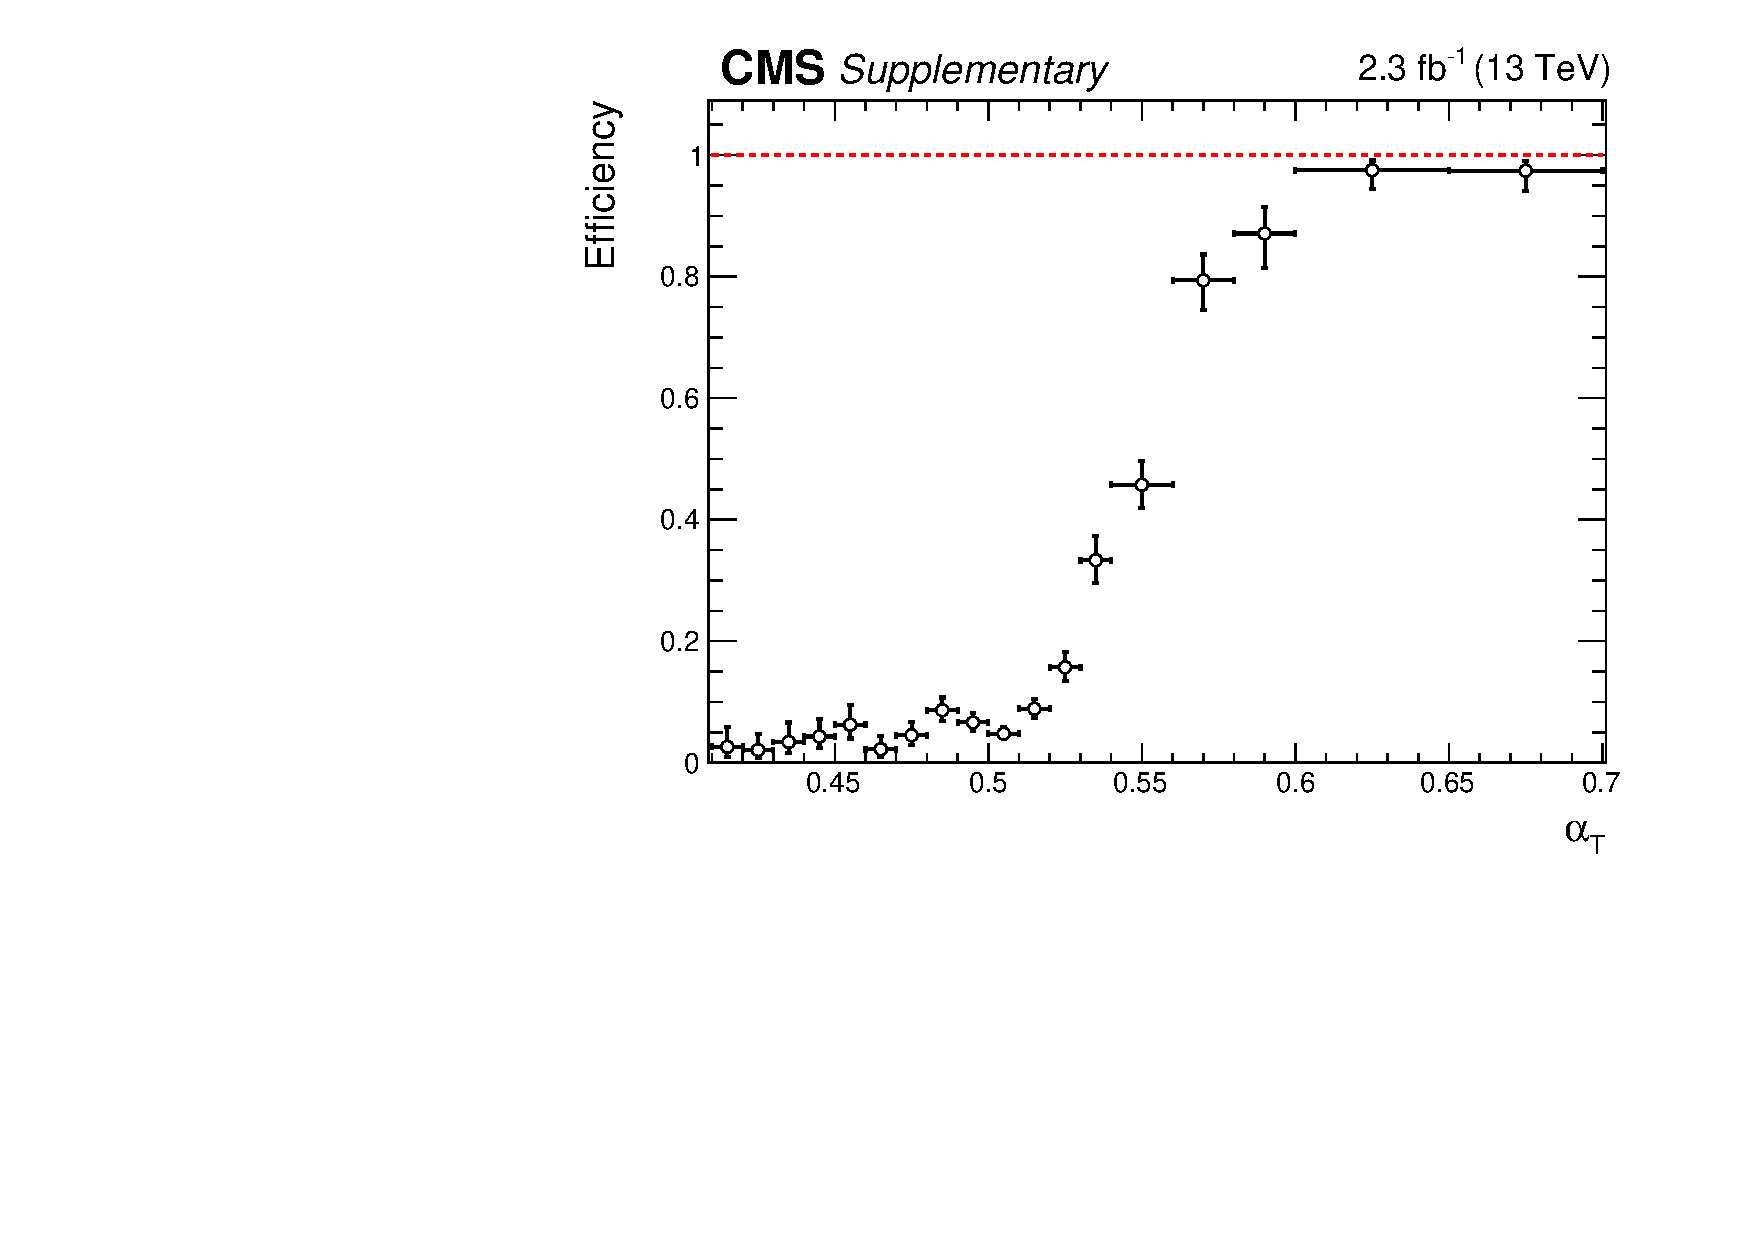
\includegraphics[width=0.48\textwidth]{figures/Trigger_HLT_PFHT200_DiPFJetAve90_PFAlphaT0p57_MoM_HT300_alphaT} } ~~
     \subfigure[{\tiny HLT\_PFHT250\_DiPFJetAve90\_PFAlphaT0p55 ($\scalht > 350 \mathrm{GeV}$)}]{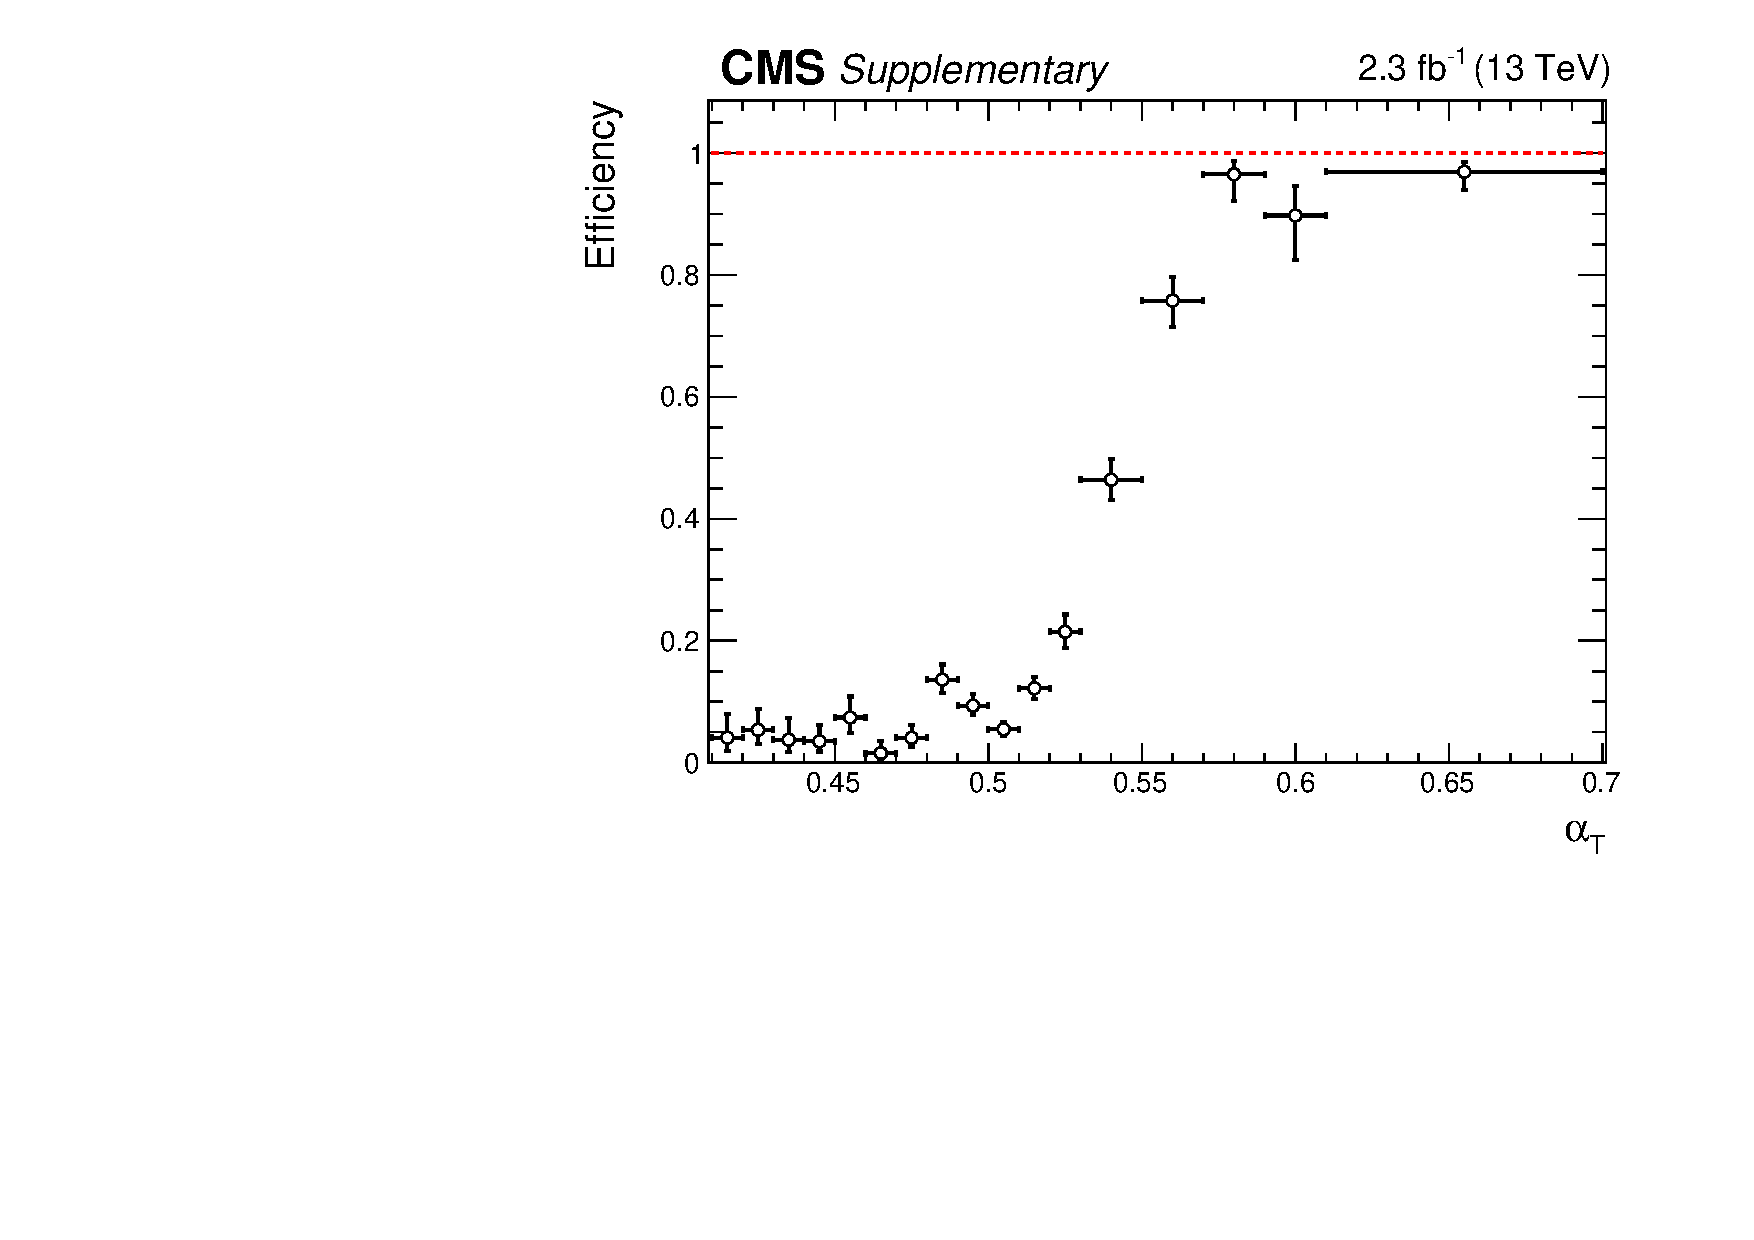
\includegraphics[width=0.48\textwidth]{figures/Trigger_HLT_PFHT250_DiPFJetAve90_PFAlphaT0p55_MoM_HT350_alphaT} }
  \end{center}
\end{figure}



\clearpage
\begin{figure}[tbhp]
    \caption{ 
    The performance of the $\Delta\phi*_{\mathrm{min}}$ variable in black compared to the ``canonical'' $\Delta\phi$ 
    considering all jets in the event ($\Delta\phi(j_{\mathrm{all}},\scalht^{miss})$) in red, 
    expressed in terms of efficiency for events from QCD and background with genuine missing transverse momentum (T1tttt model) 
    for several cut values, on the left (right) plot. 
    The black and red stars identify respectively the $\Delta\phi*_{\mathrm{min}}>0.5$ and $\Delta\phi(j_{\mathrm{all}},\scalht^{miss})>0.5$ working points. 
    \label{fig:bDPhi-ROC} }
  \begin{center}
     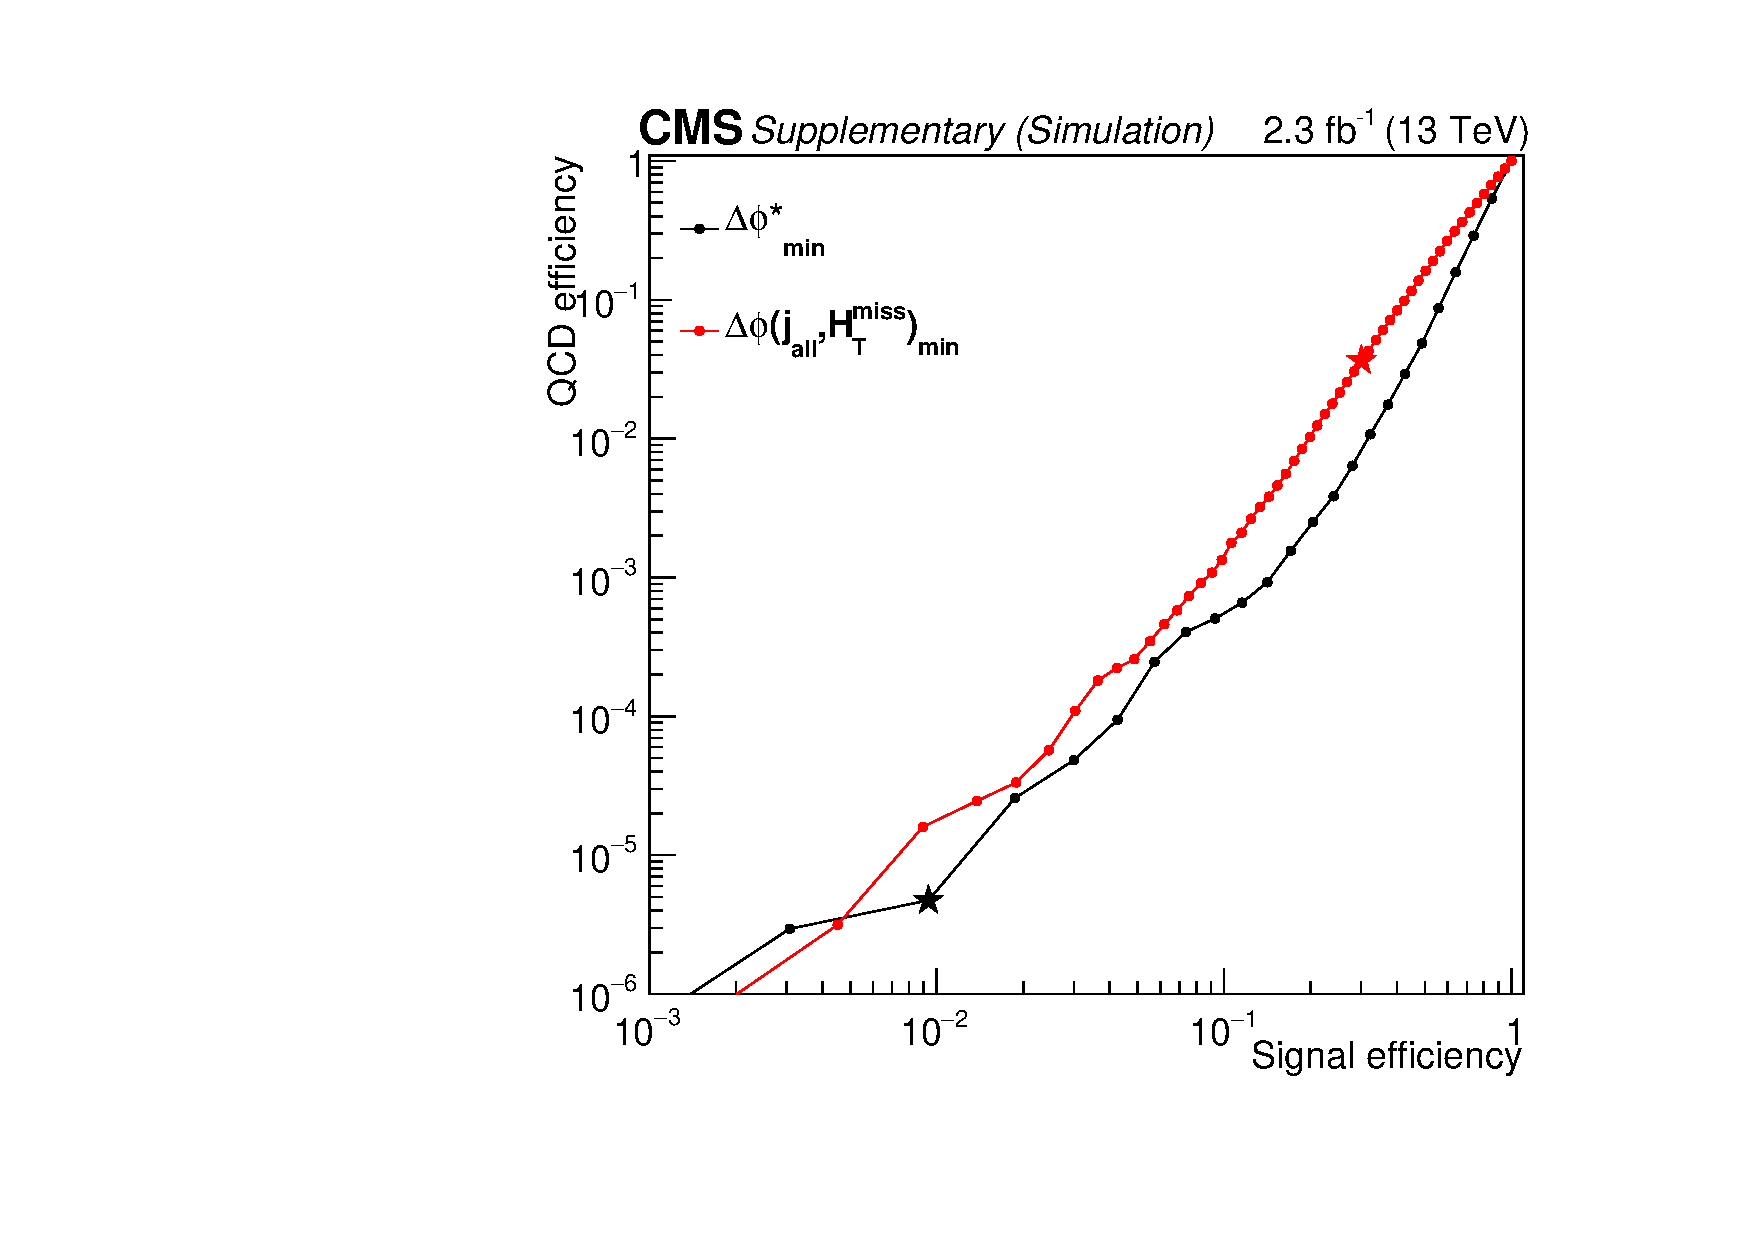
\includegraphics[width=0.48\textwidth]{figures/ewk_ht800} ~~
     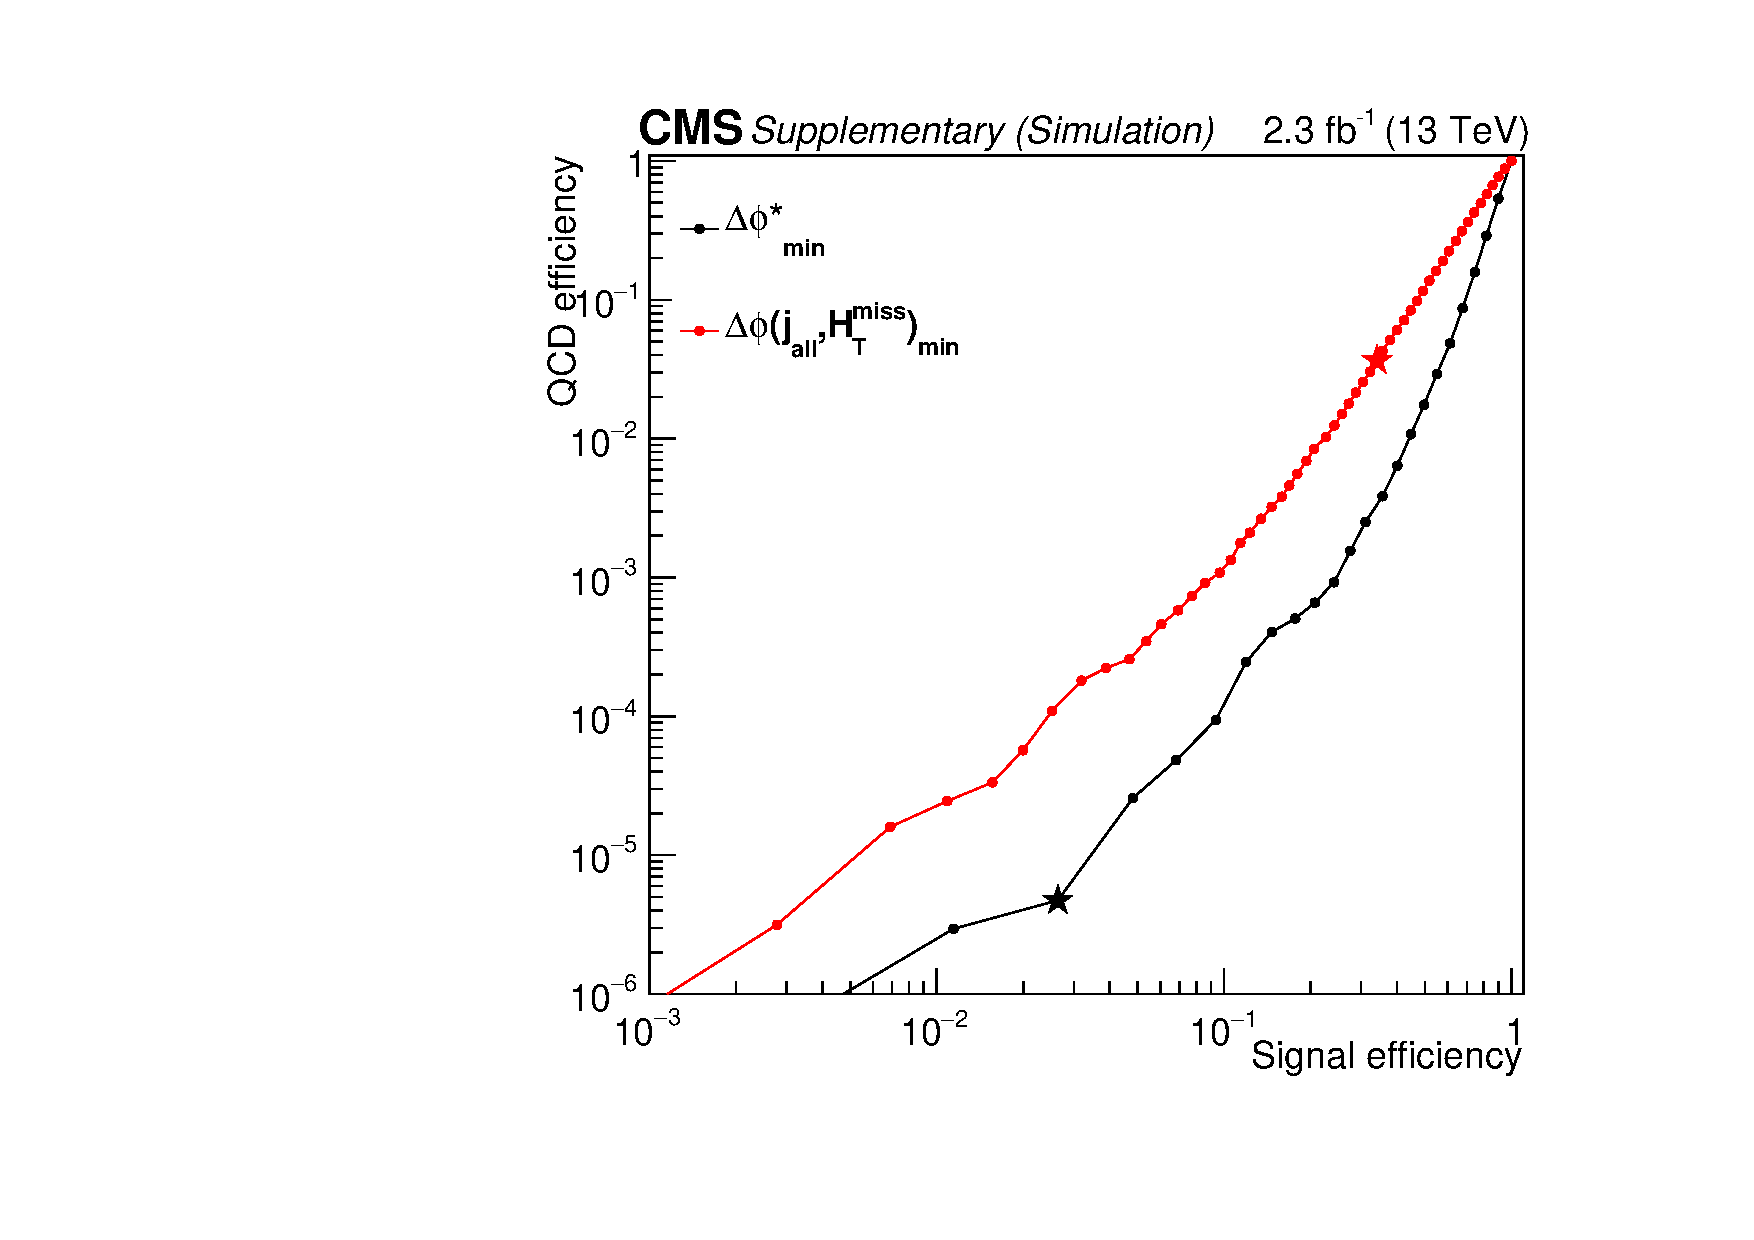
\includegraphics[width=0.48\textwidth]{figures/T1tttt_uncomp_ht800}
  \end{center}
\end{figure}



\clearpage
\begin{figure}[tbhp]
    \caption{ 
    Distributions of data and MC predictions for \scalht (top left), \mht (top right), \nj (bottom left) and \nb (bottom right) 
    for the $\mu+\mathrm{jets}$ control region. 
    The analysis doesn't rely directly on simulation to derive the backgrounds, 
    so these plots are meant to show the shape of some of the variables used in the analysis despite the limitations 
    of the MC modelling. 
    \label{fig:data-MC_plots_SingleMu} }
  \begin{center}
     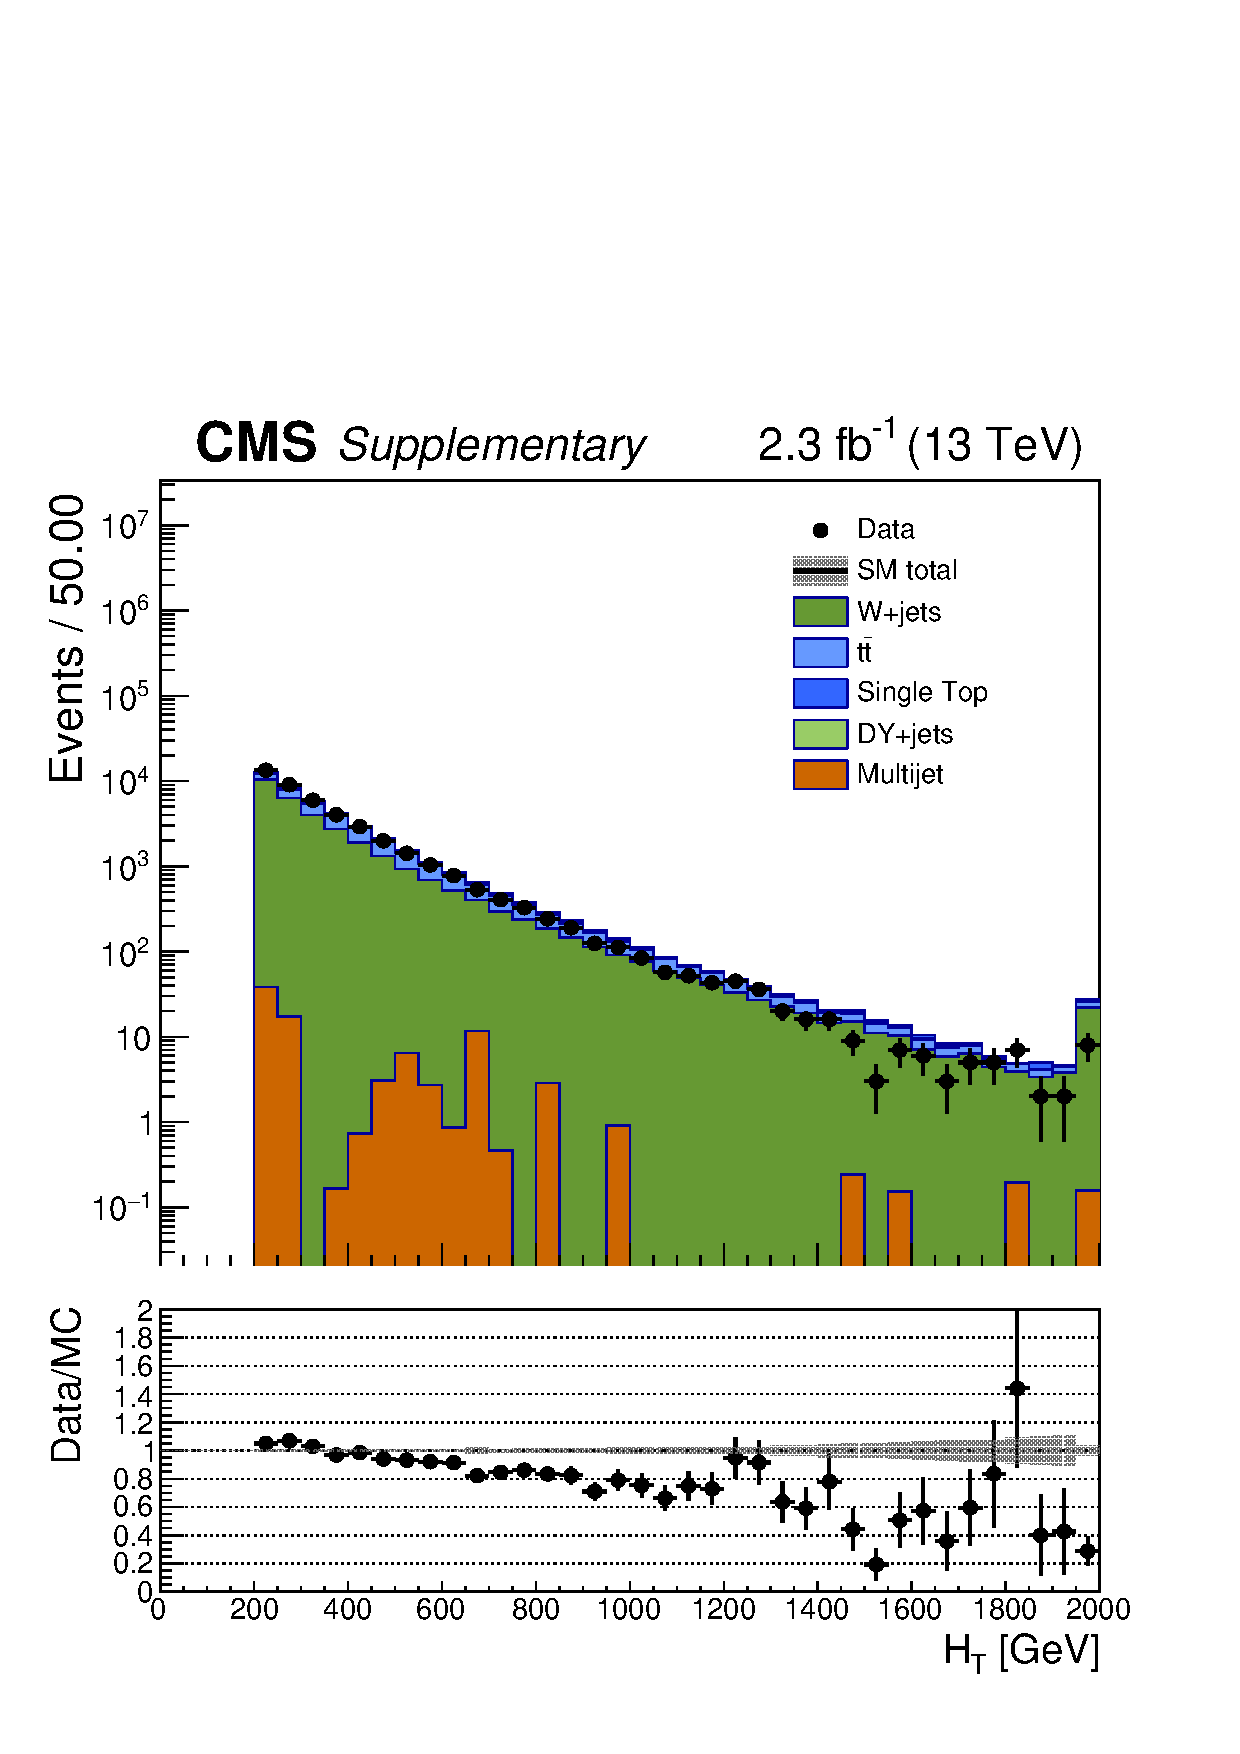
\includegraphics[width=0.45\textwidth]{figures/SingleMu_ht40_all_all} ~~
     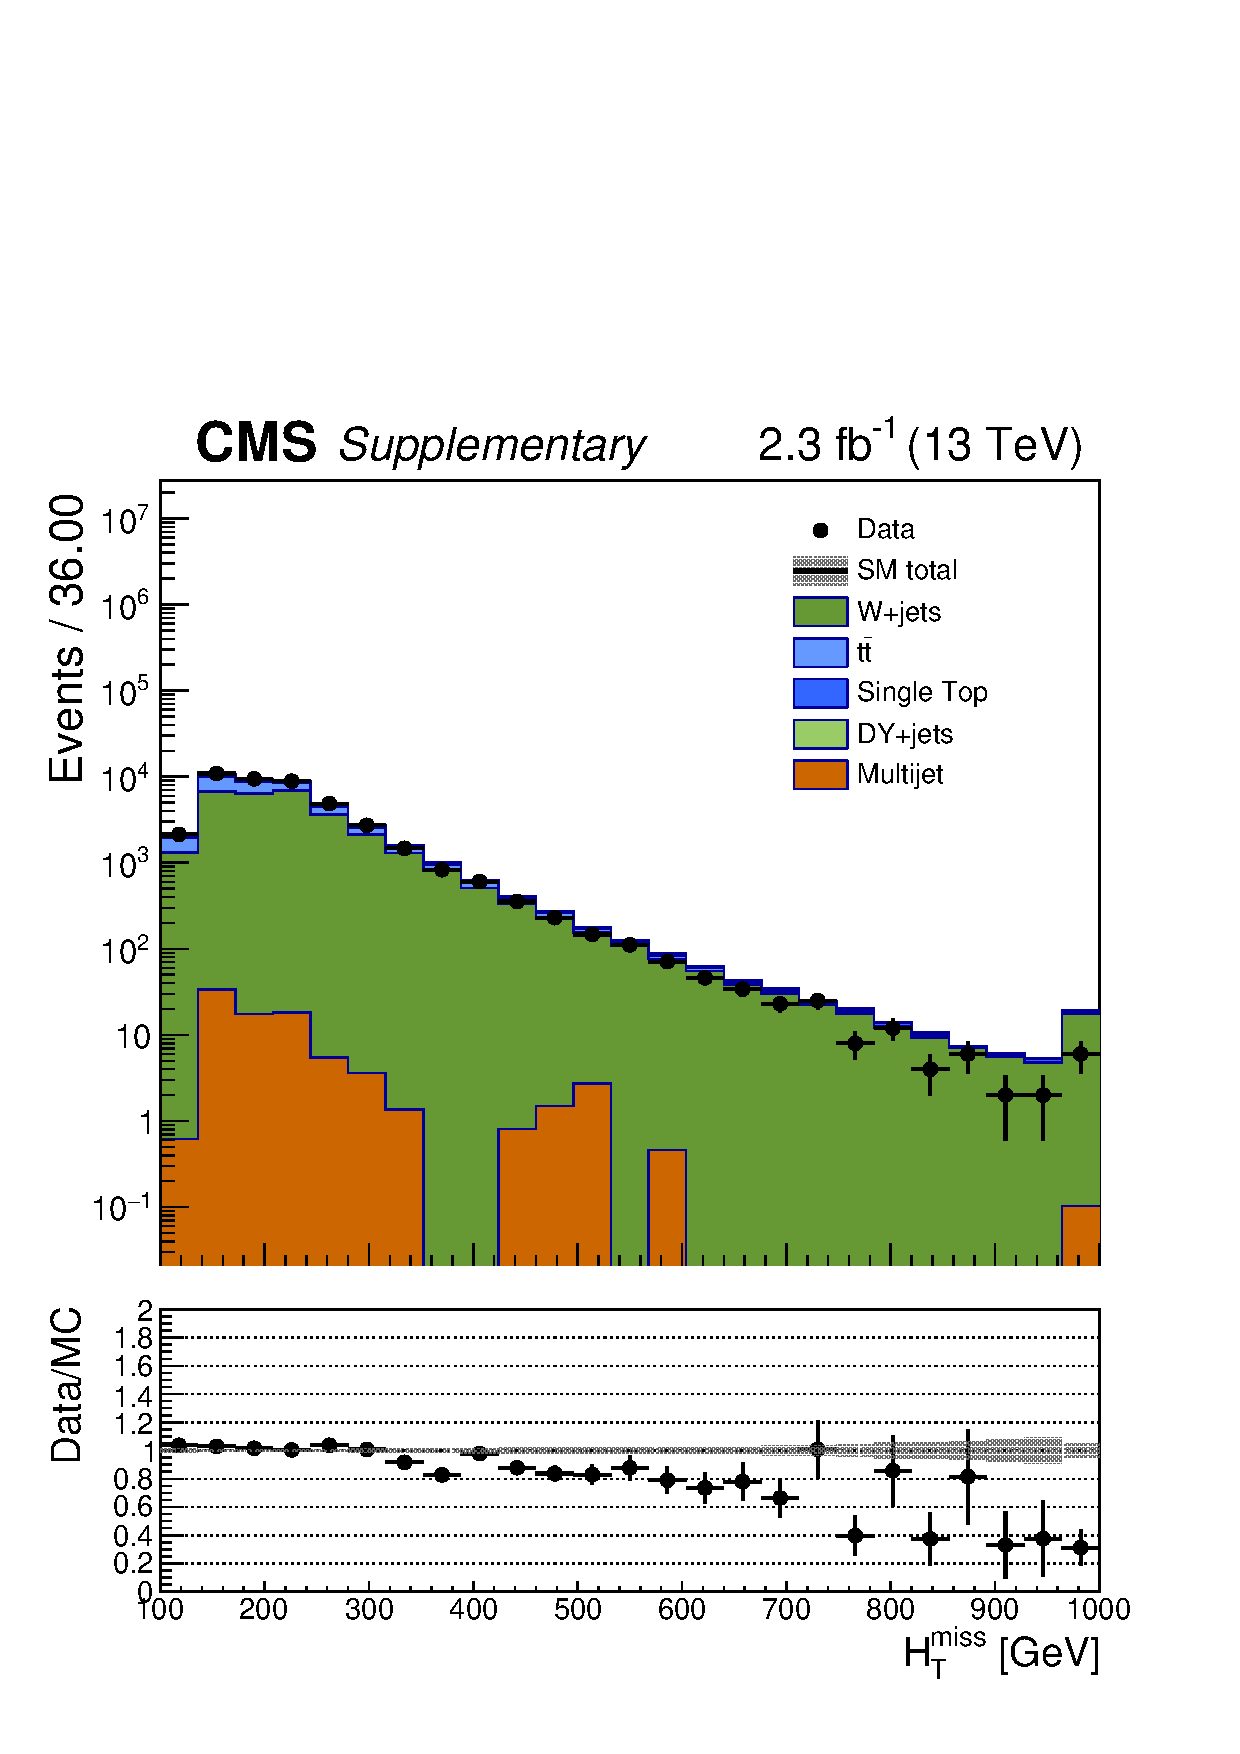
\includegraphics[width=0.45\textwidth]{figures/SingleMu_mht40_pt_all_all} \\
     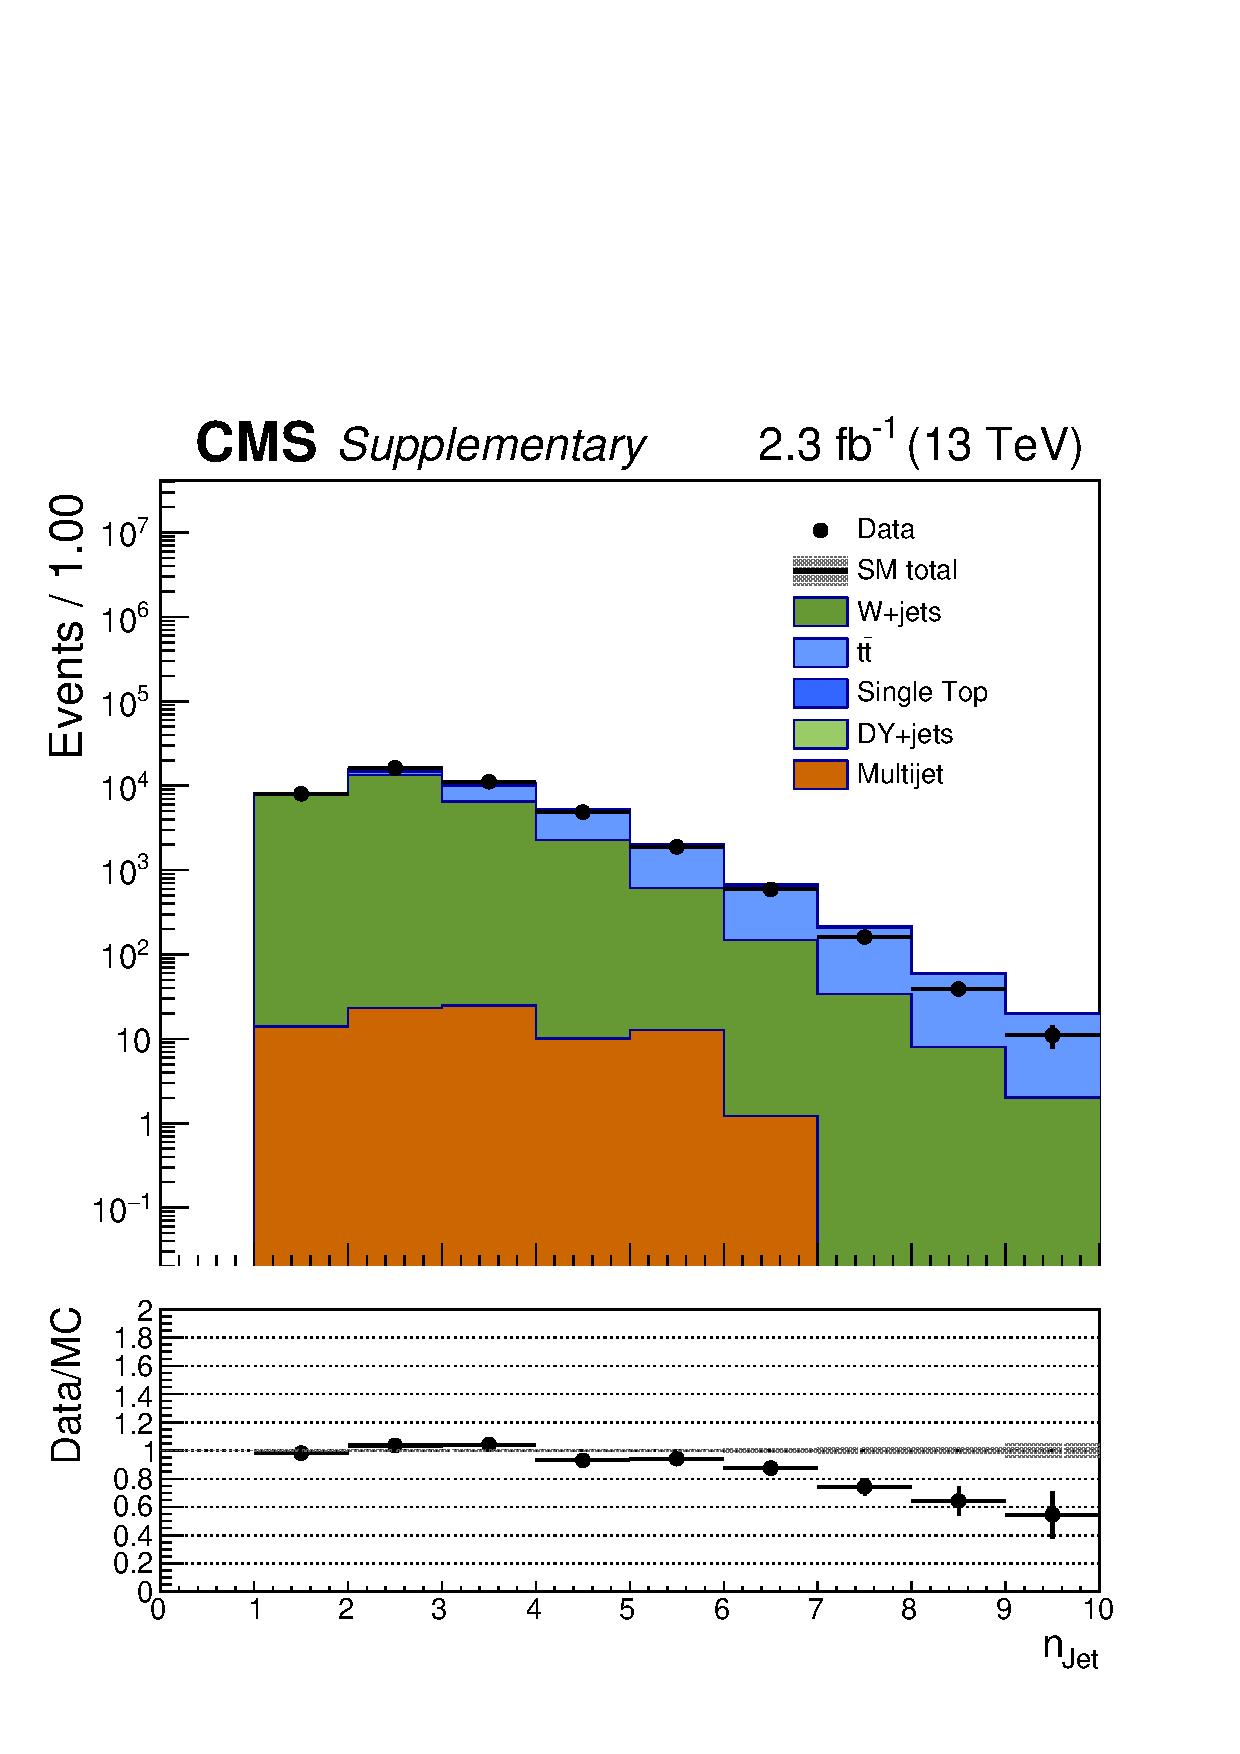
\includegraphics[width=0.45\textwidth]{figures/SingleMu_nJet40_all_all} ~~
     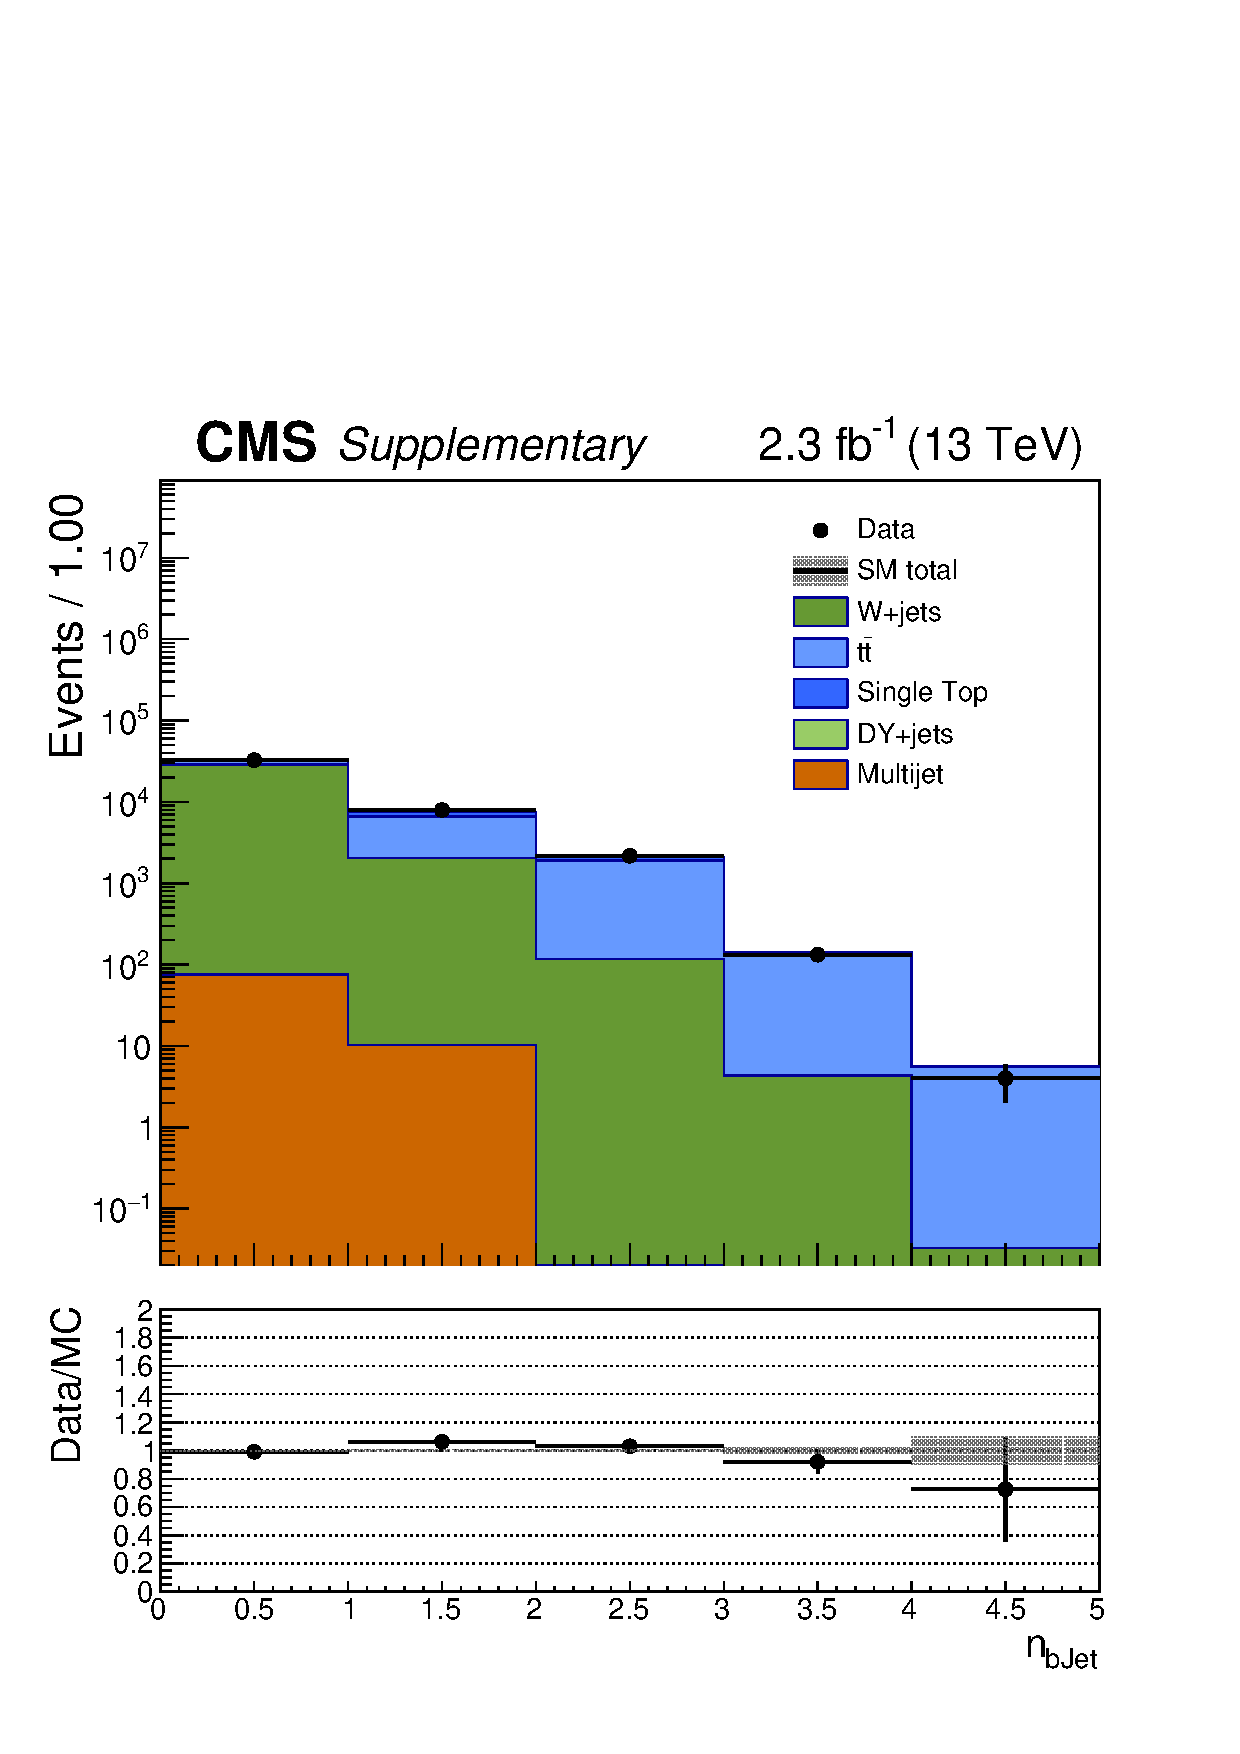
\includegraphics[width=0.45\textwidth]{figures/SingleMu_nBJet40_all_all} \\
  \end{center}
\end{figure}



\clearpage
\begin{figure}[tbhp]
    \caption{ 
    Distributions of data and MC predictions for \scalht (top left), \mht (top right), \nj (bottom left) and \nb (bottom right) 
    for the $\gamma+\mathrm{jets}$ control region. 
    The analysis doesn't rely directly on simulation to derive the backgrounds, 
    so these plots are meant to show the shape of some of the variables used in the analysis despite the limitations 
    of the MC modelling. 
    \label{fig:data-MC_plots_SinglePhoton} }
  \begin{center}
     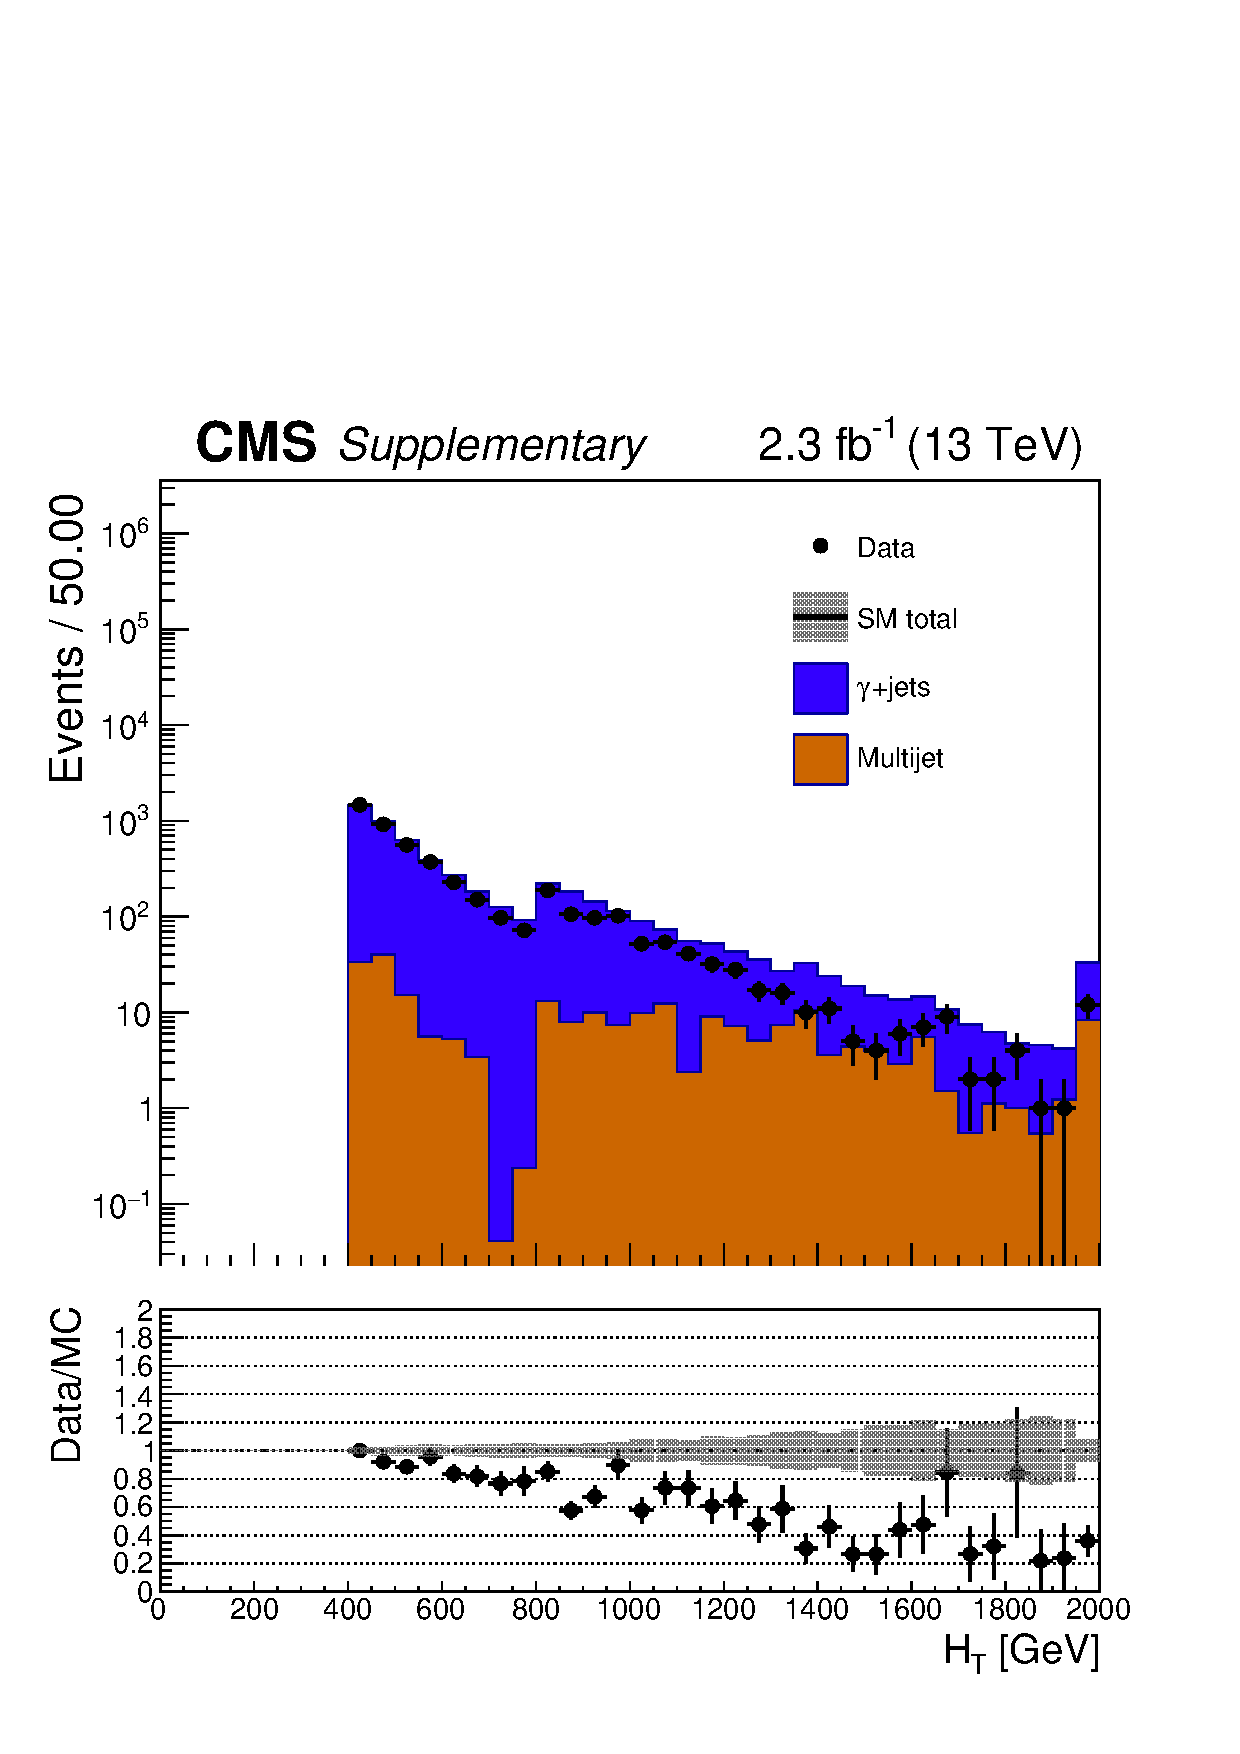
\includegraphics[width=0.45\textwidth]{figures/SinglePhoton_ht40_all_all} ~~
     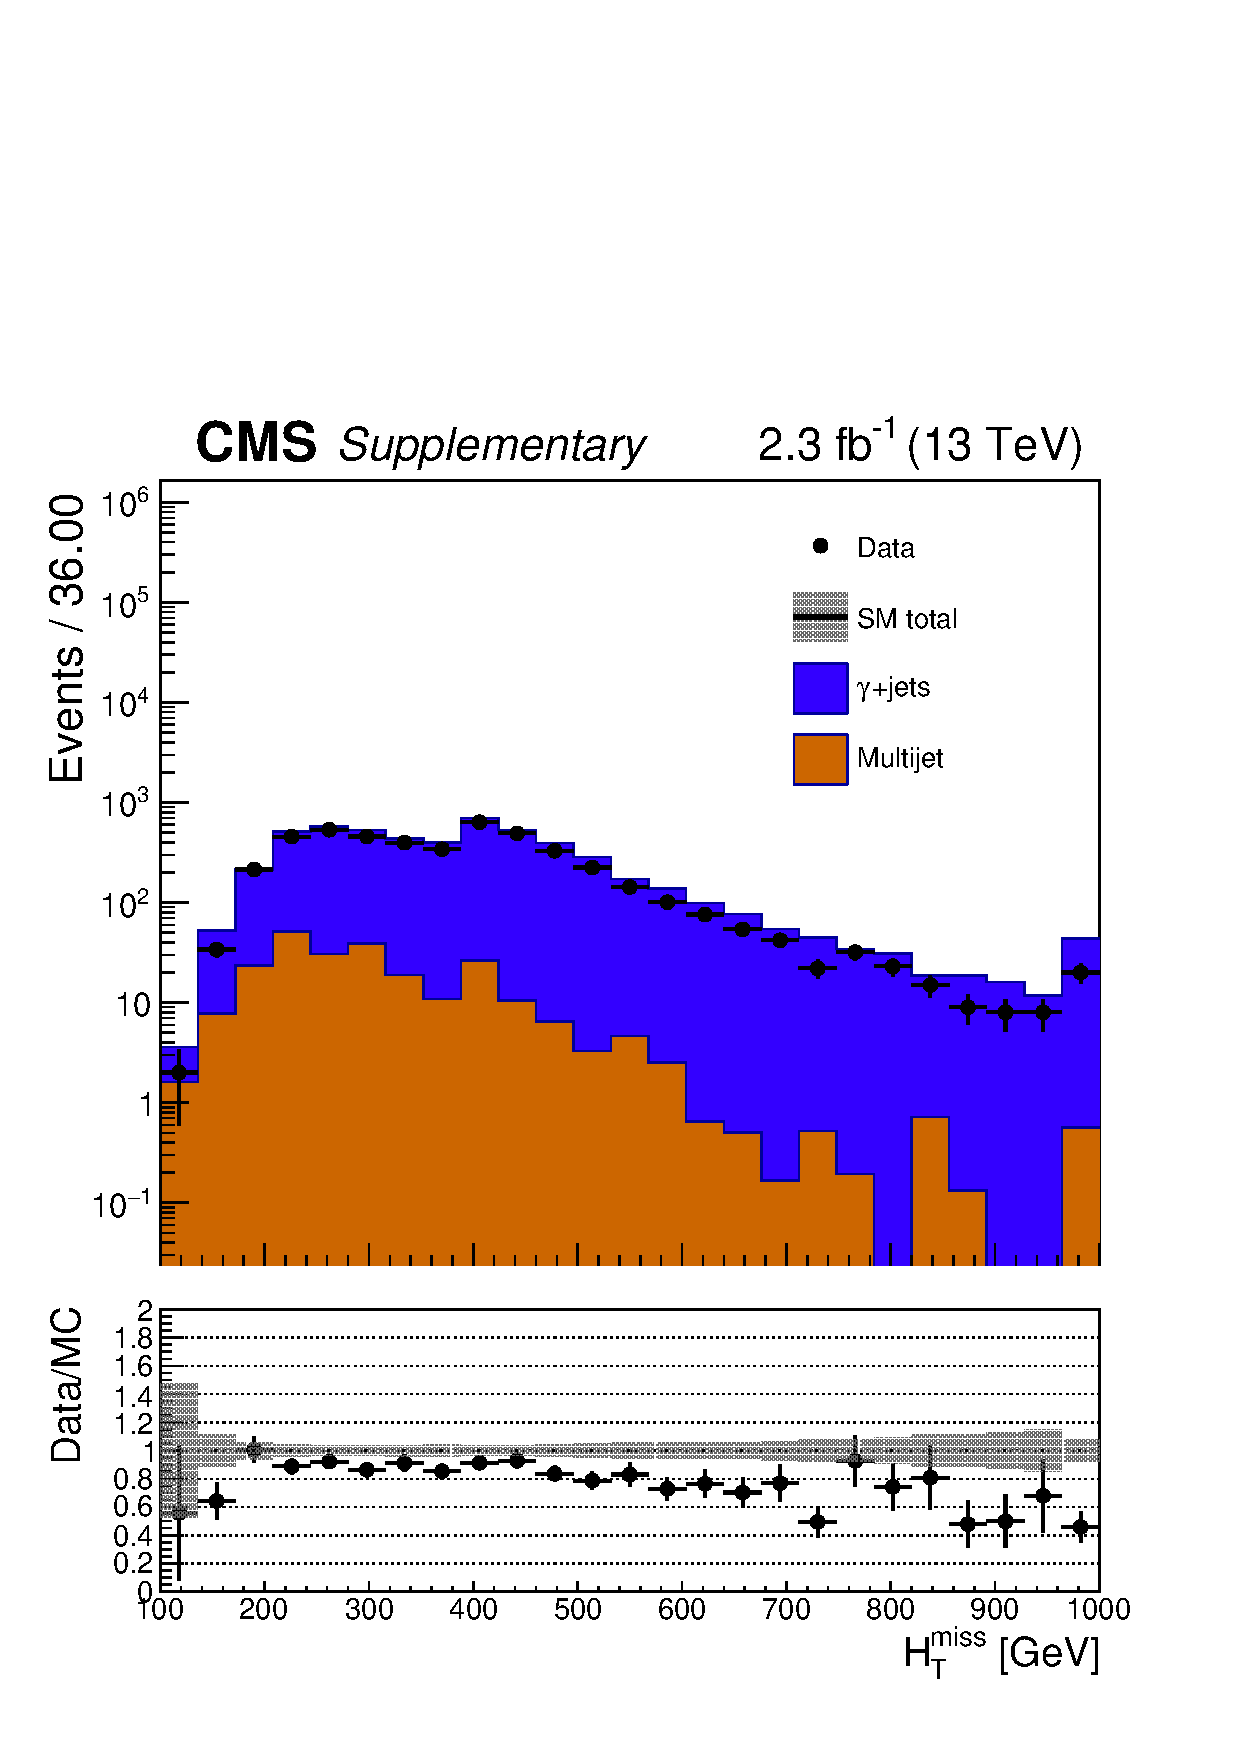
\includegraphics[width=0.45\textwidth]{figures/SinglePhoton_mht40_pt_all_all} \\
     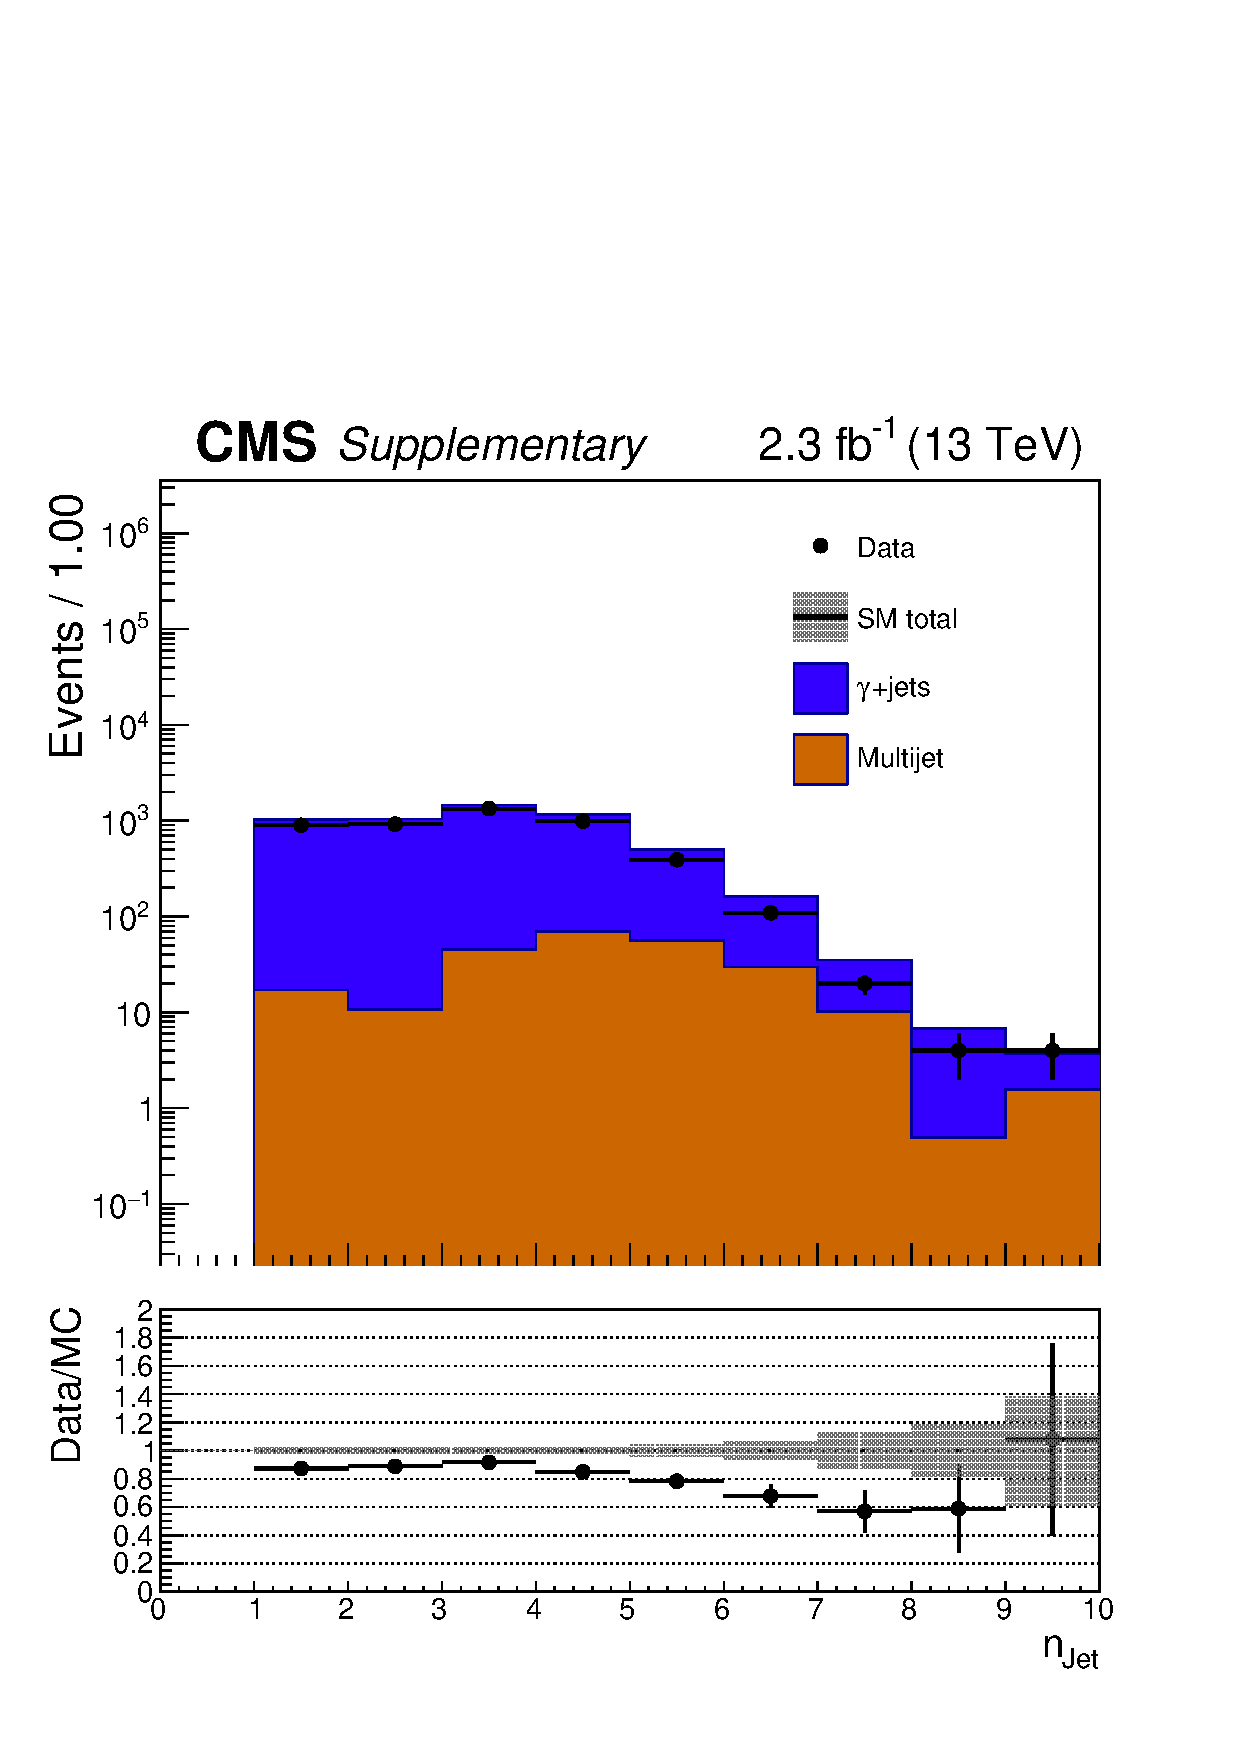
\includegraphics[width=0.45\textwidth]{figures/SinglePhoton_nJet40_all_all} ~~
     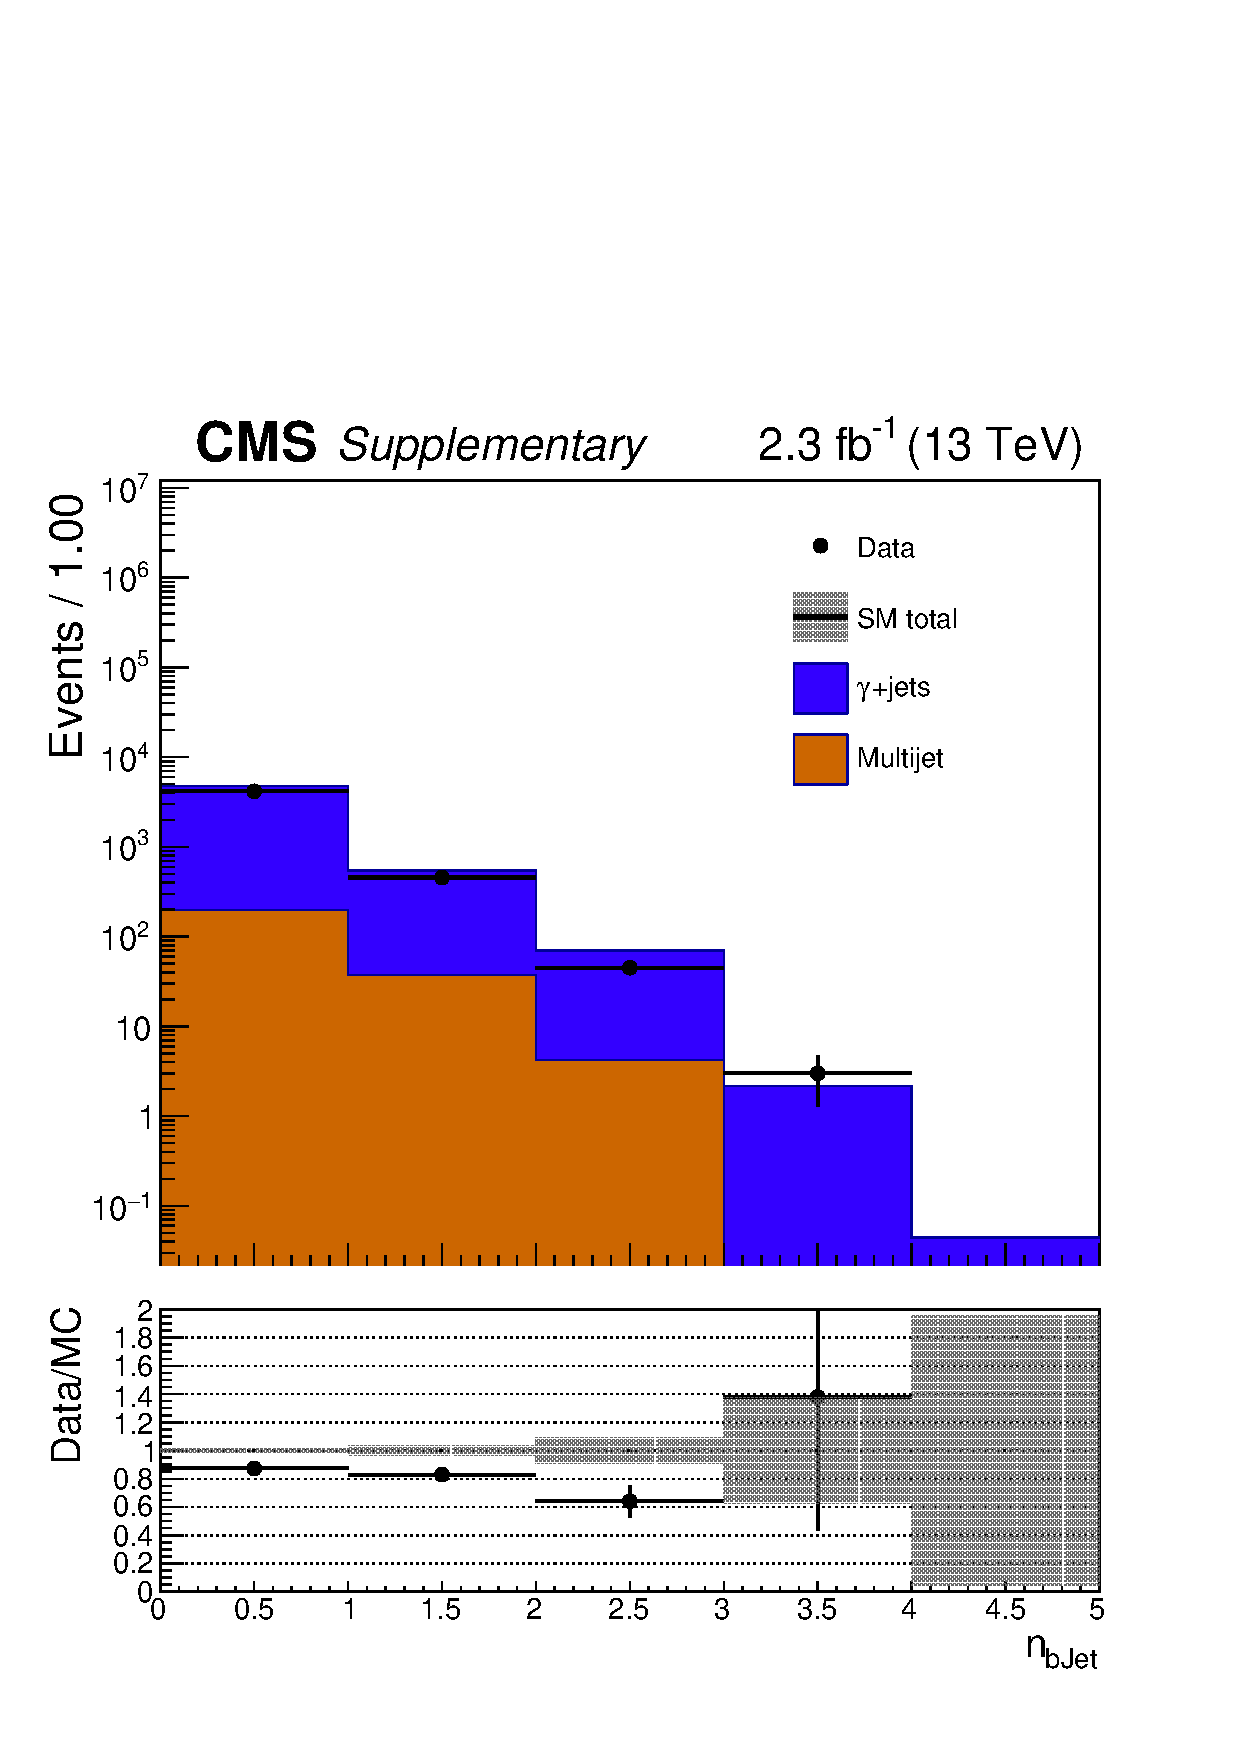
\includegraphics[width=0.45\textwidth]{figures/SinglePhoton_nBJet40_all_all} \\
  \end{center}
\end{figure}


\clearpage
\begin{figure}[tbhp]
    \caption{ 
    Distributions of data and MC predictions for \scalht (top left), \mht (top right), \nj (bottom left) and \nb (bottom right) 
    for the $\mu\mu+\mathrm{jets}$ control region. 
    The analysis doesn't rely directly on simulation to derive the backgrounds, 
    so these plots are meant to show the shape of some of the variables used in the analysis despite the limitations 
    of the MC modelling. 
    \label{fig:data-MC_plots_DoubleMu} }
  \begin{center}
     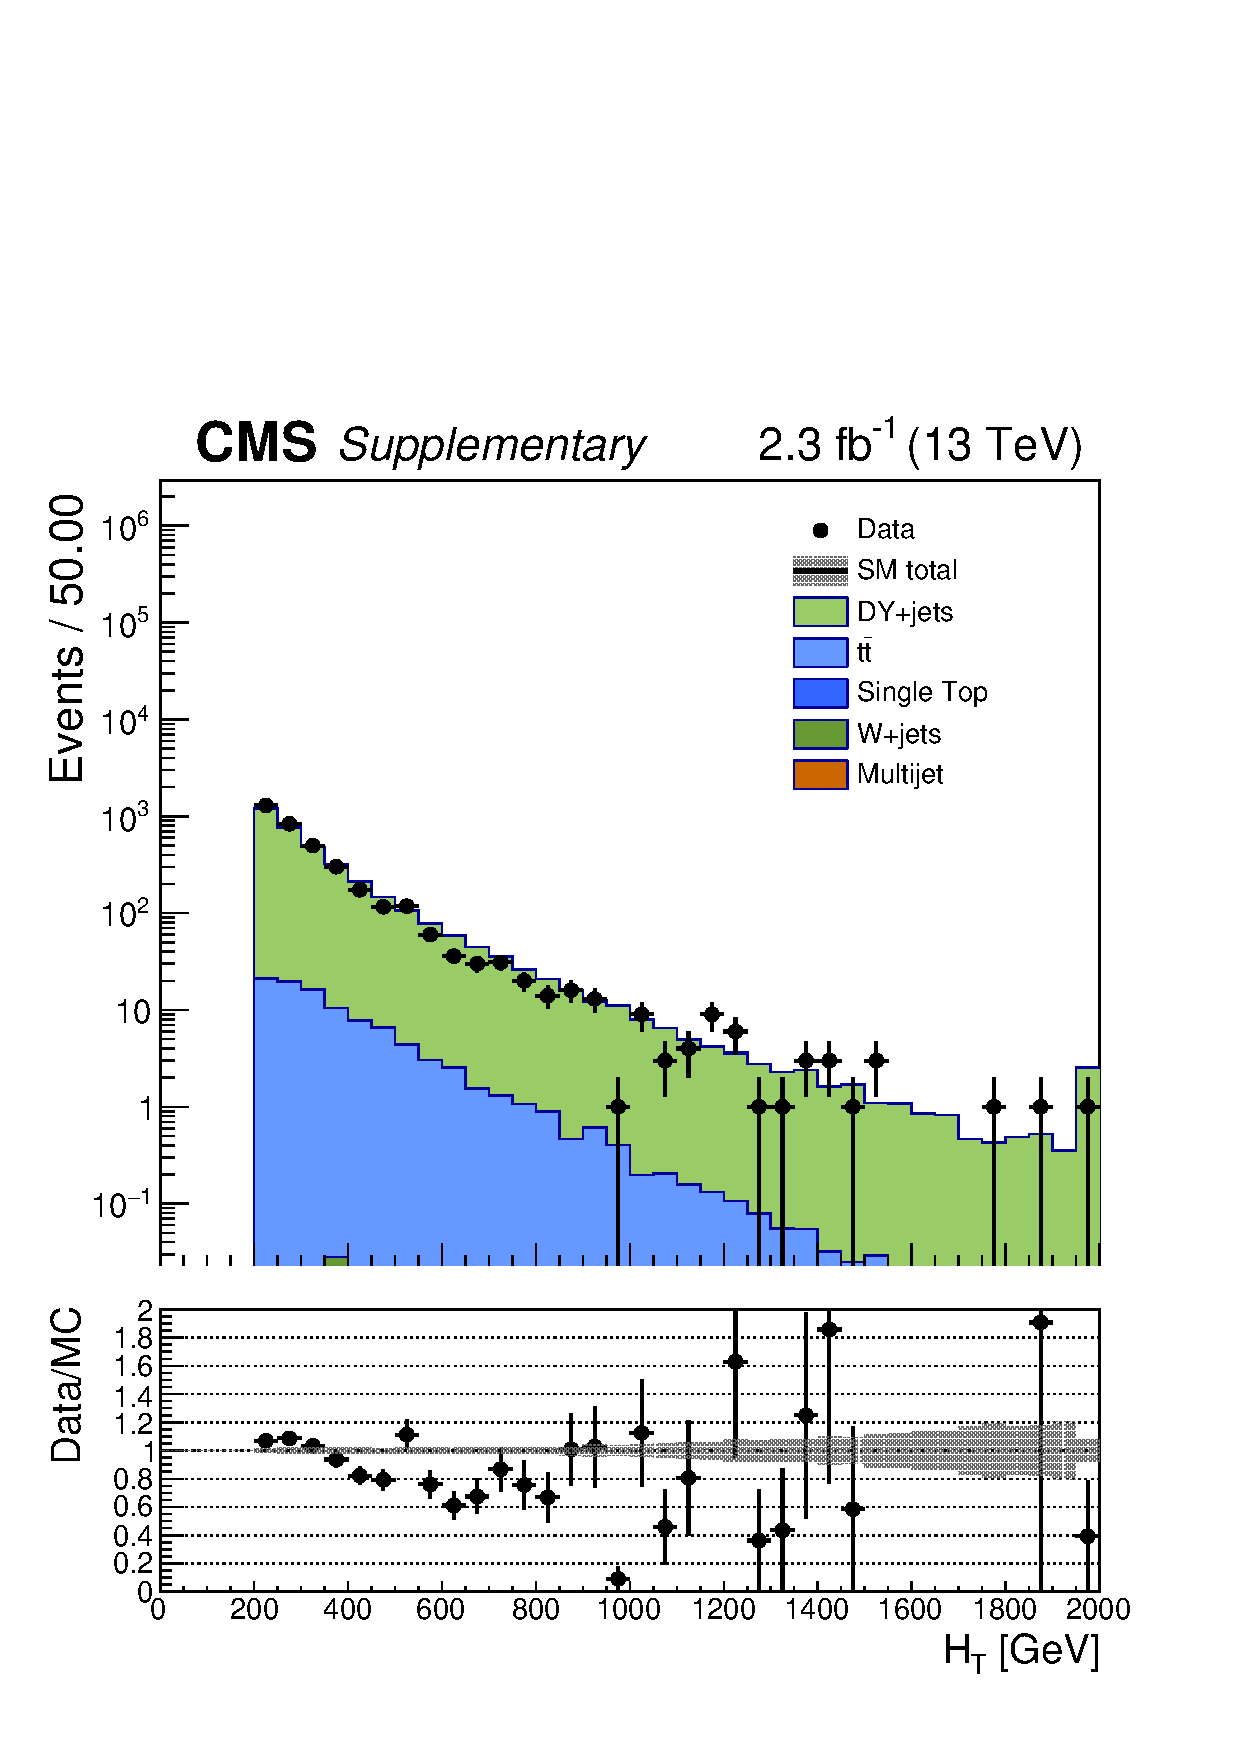
\includegraphics[width=0.45\textwidth]{figures/DoubleMu_ht40_all_all} ~~
     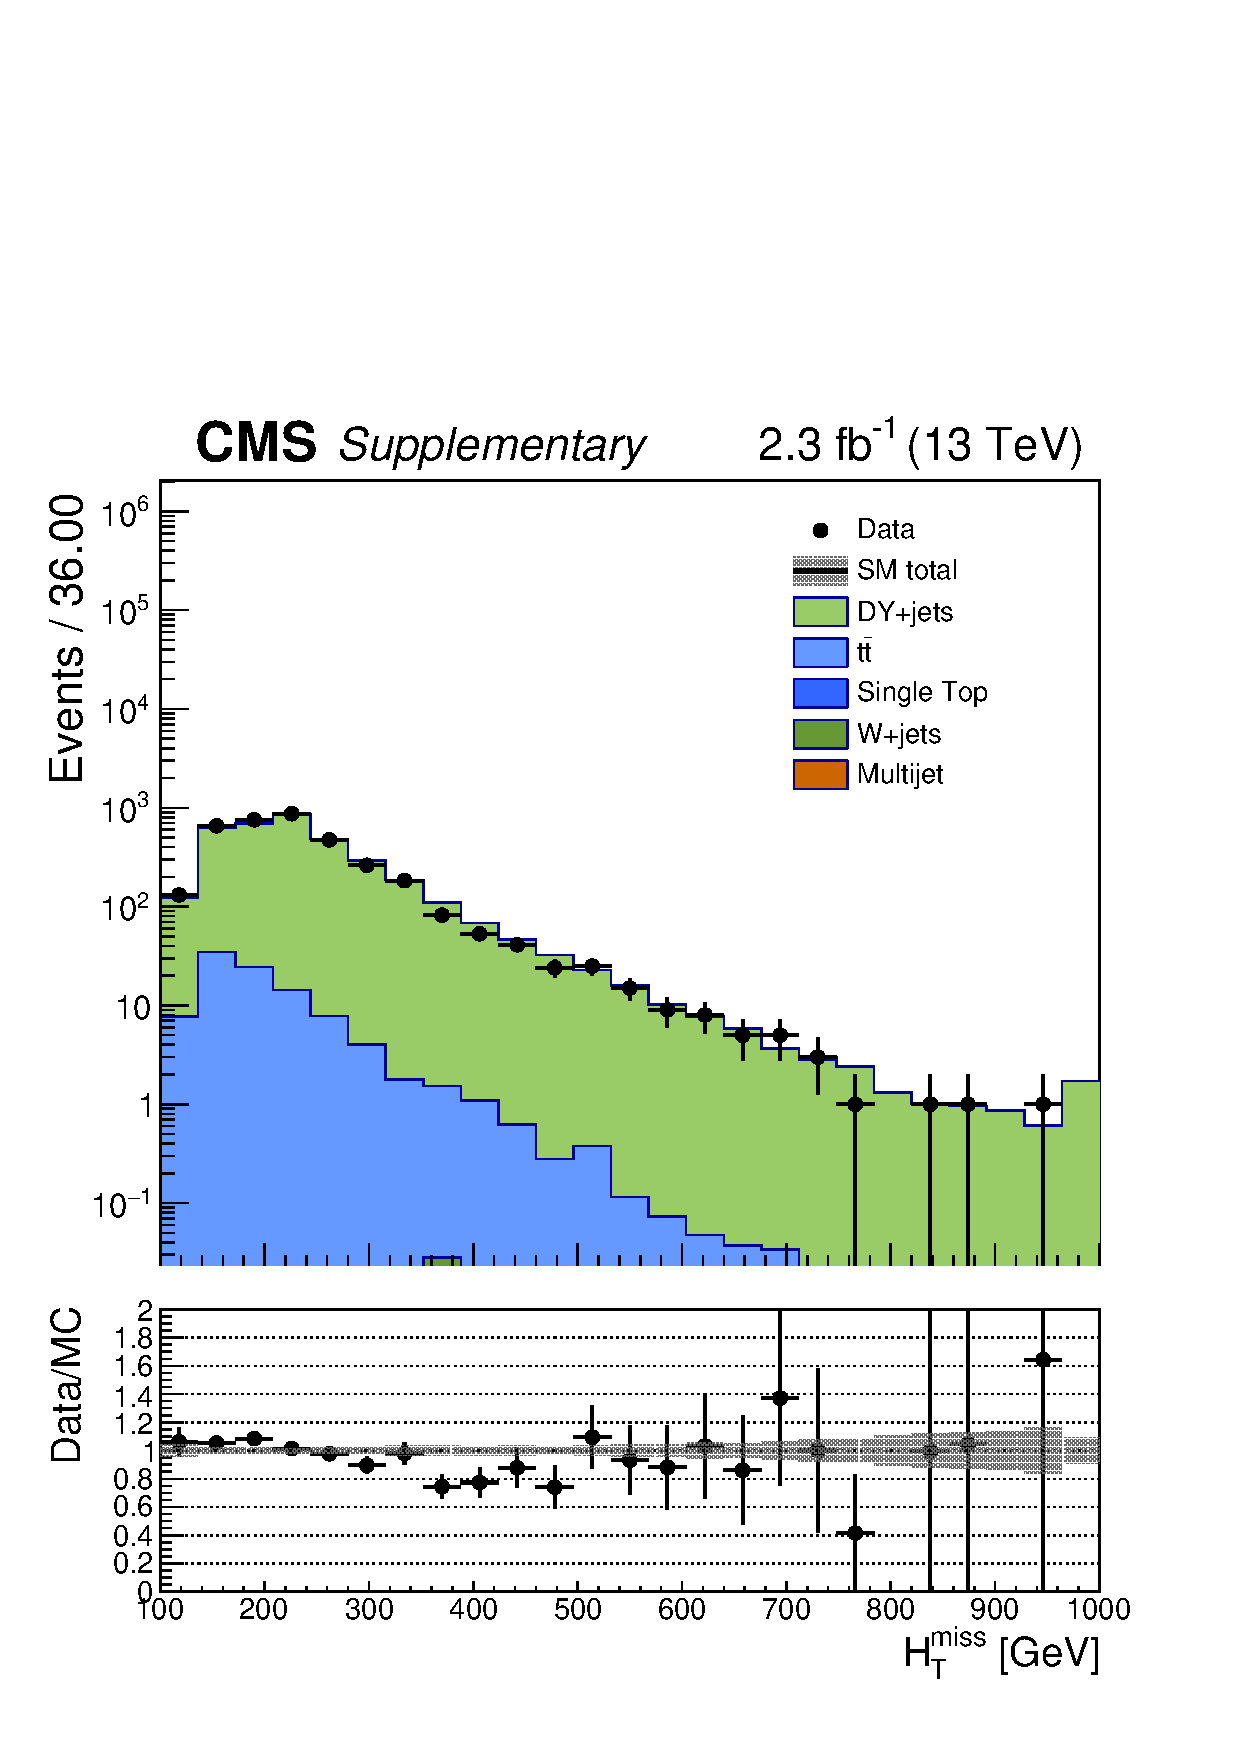
\includegraphics[width=0.45\textwidth]{figures/DoubleMu_mht40_pt_all_all} \\
     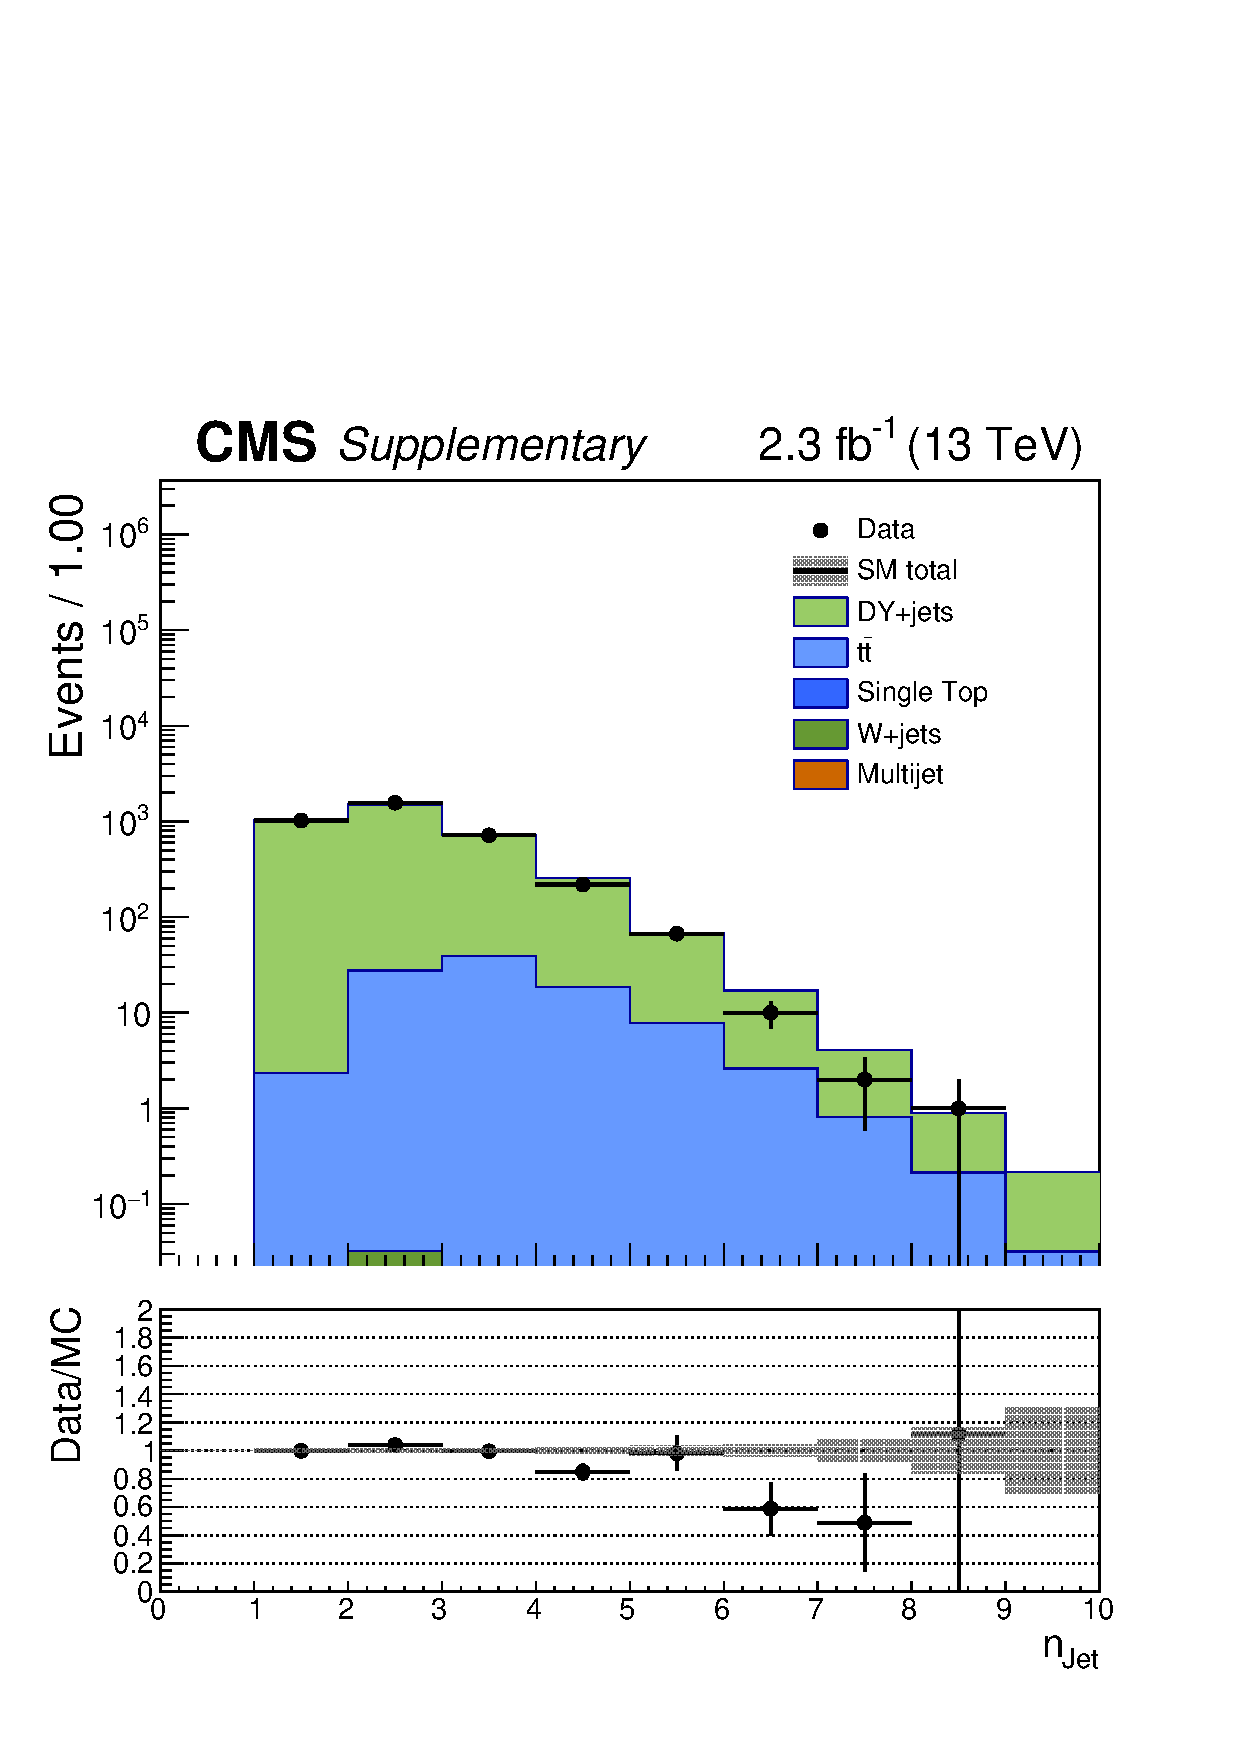
\includegraphics[width=0.45\textwidth]{figures/DoubleMu_nJet40_all_all} ~~
     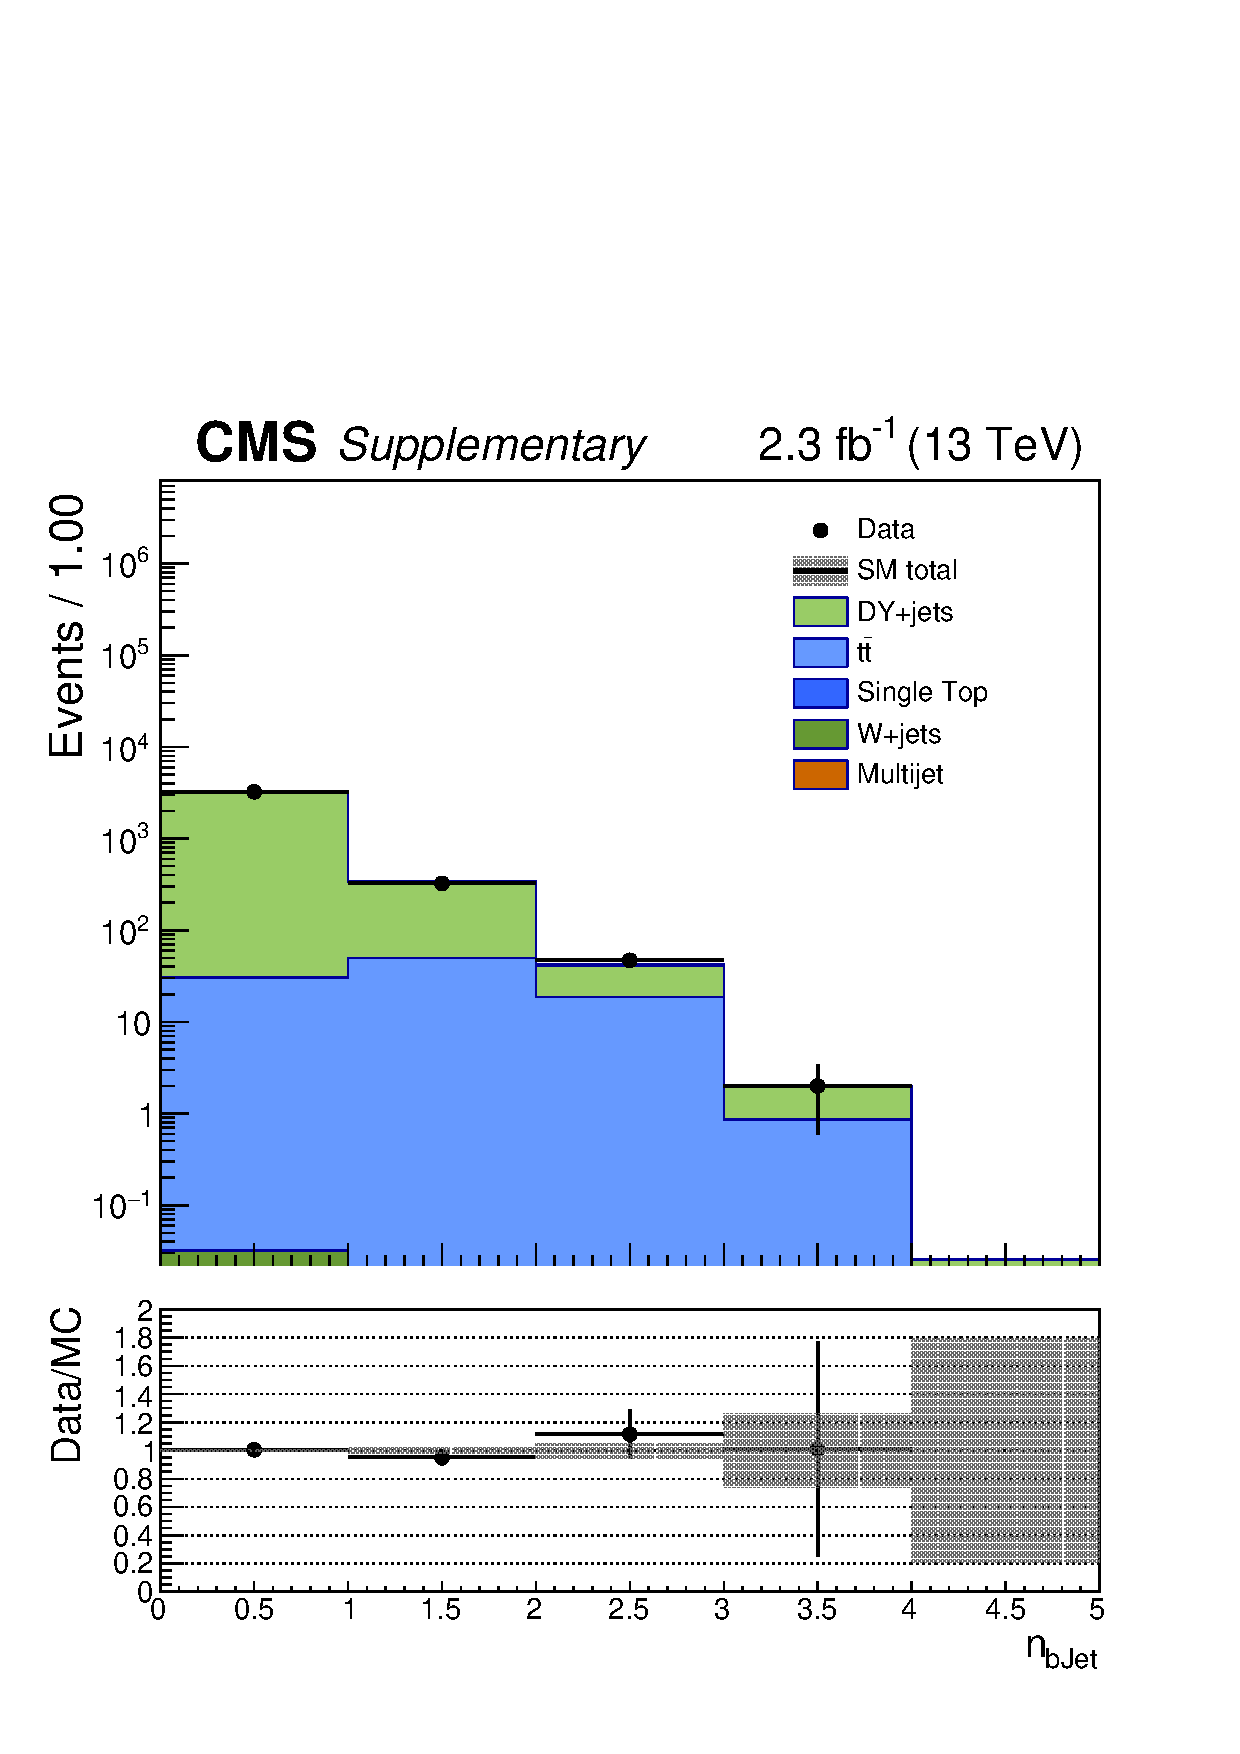
\includegraphics[width=0.45\textwidth]{figures/DoubleMu_nBJet40_all_all} \\
  \end{center}
\end{figure}


\clearpage
\begin{figure}[tbhp]
    \caption{ 
    The relative contribution of the multi-jet component to the sum of the non multi-jet backgrounds 
    as a function of the \scalht bin (x-axis) and \nj bin (y-axis). 
    The empty bins are not used in the analysis because they are kinematically not accessible. 
    \label{fig:qcd-rel-cont} }
  \begin{center}
     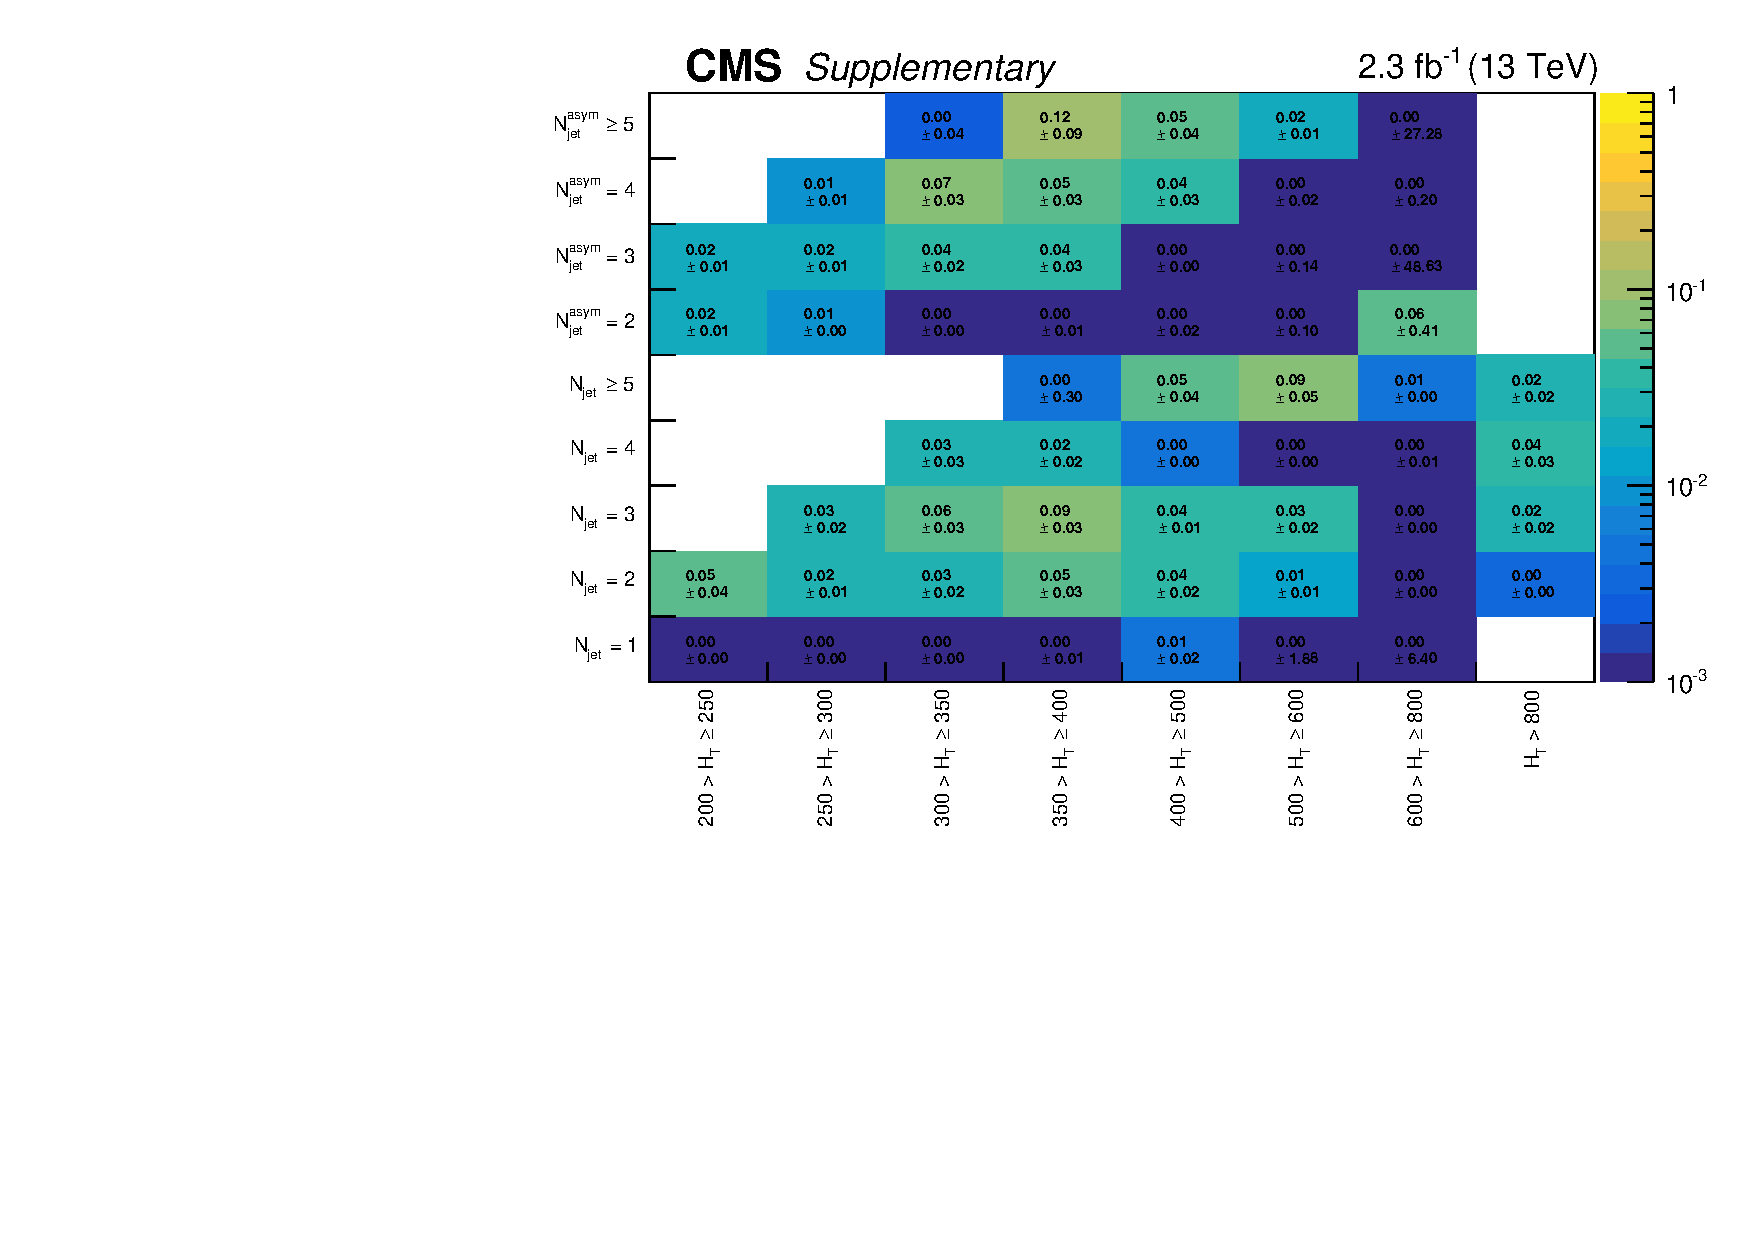
\includegraphics[width=0.5\textwidth]{figures/QCDRelCont}
  \end{center}
\end{figure}



\clearpage
\begin{figure}[tbhp]
    \caption{ 
  Data-derived test of the \alt extrapolation for the symmetric (left) and asymmetric (right) jet categories. 
  In this test, the data yield in the \mj sample with $\alt>0.5$ ($N_{\mathrm{obs}}$) 
  is compared with the prediction obtained from the \mj sample with $\alt<0.5$ multiplied by the corresponding 
  transfer factor computed in simulation ($N_{\mathrm{pred}}$). 
  A systematic uncertainty (grey band) is derived, as a function of \scalht and separately for symmetric and asymmetric categories, 
  to cover the non-closure. 
    \label{fig:CT-alphaT} }
  \begin{center}
     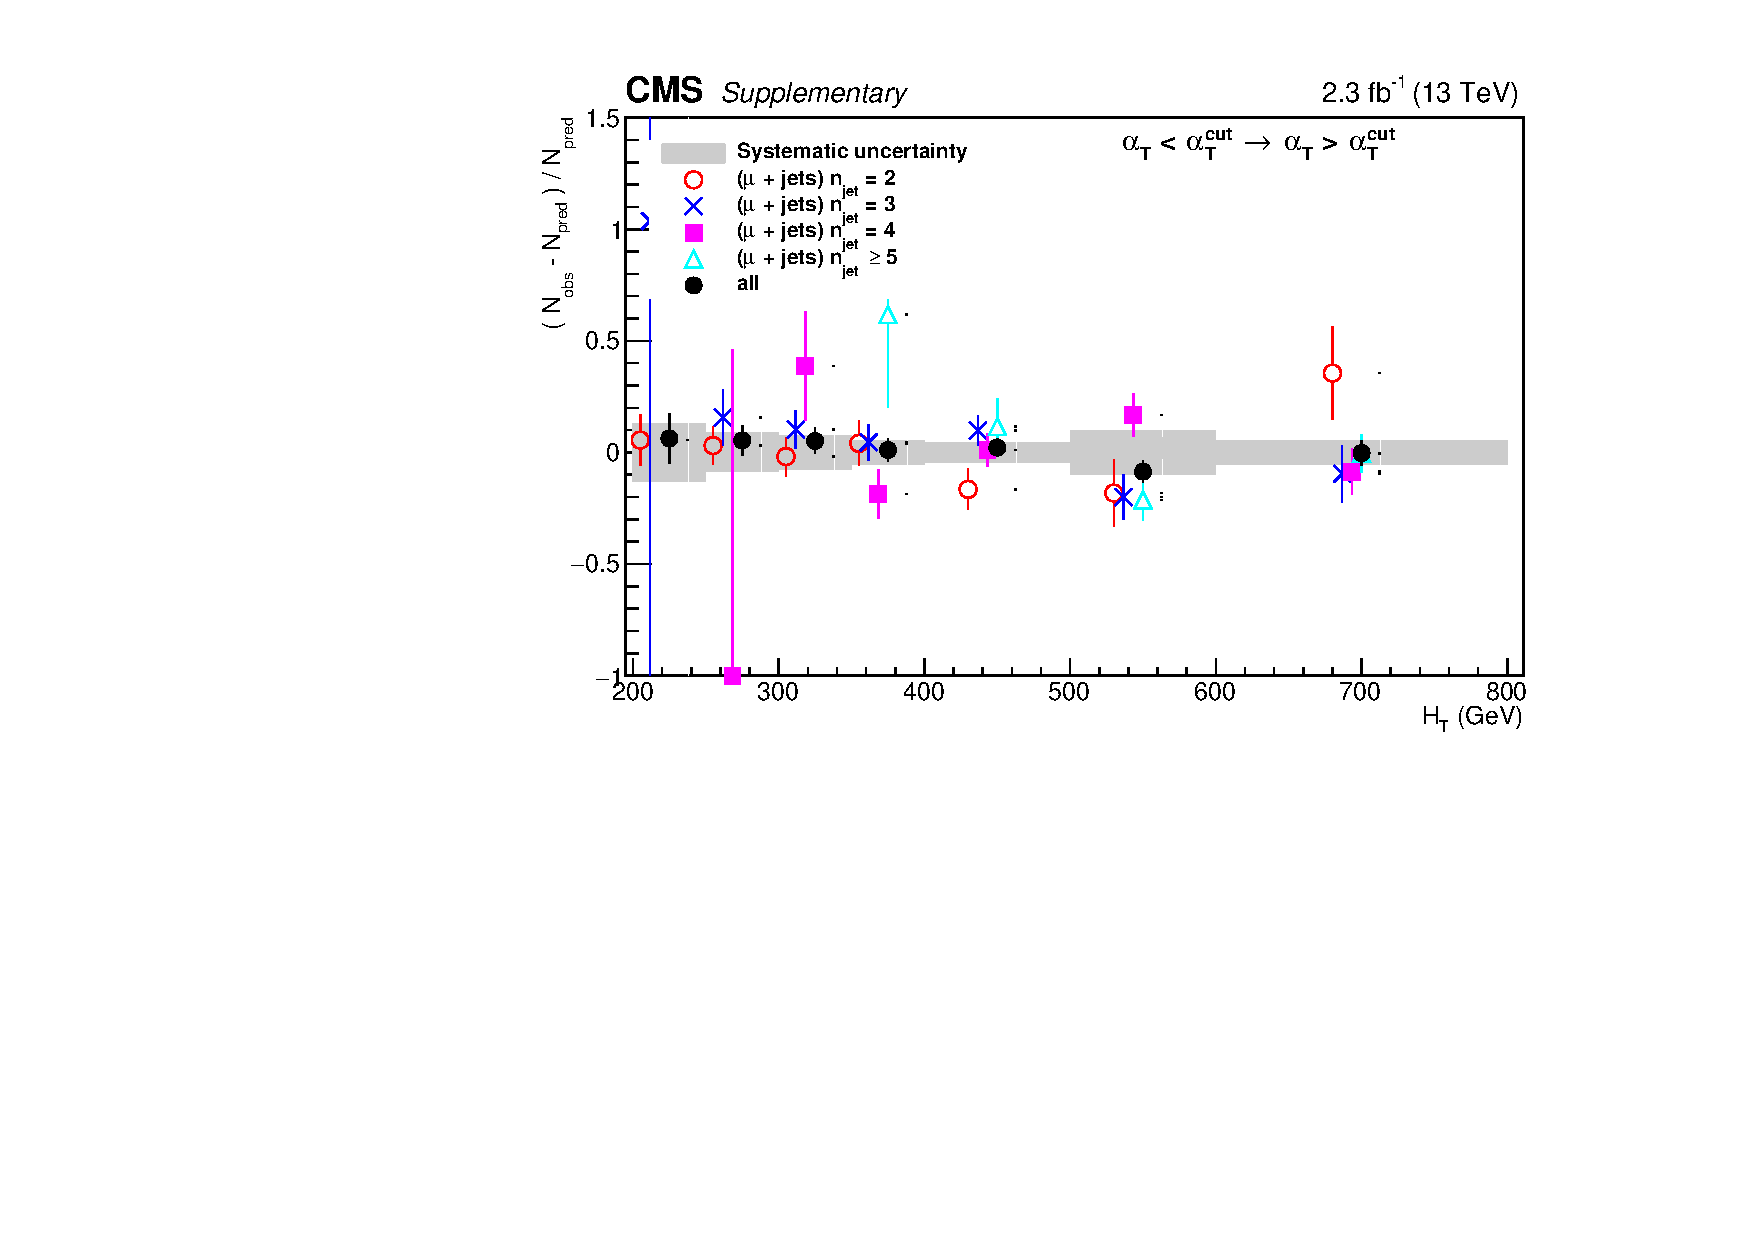
\includegraphics[width=0.48\textwidth]{figures/alphaTsym__noFit} ~~
     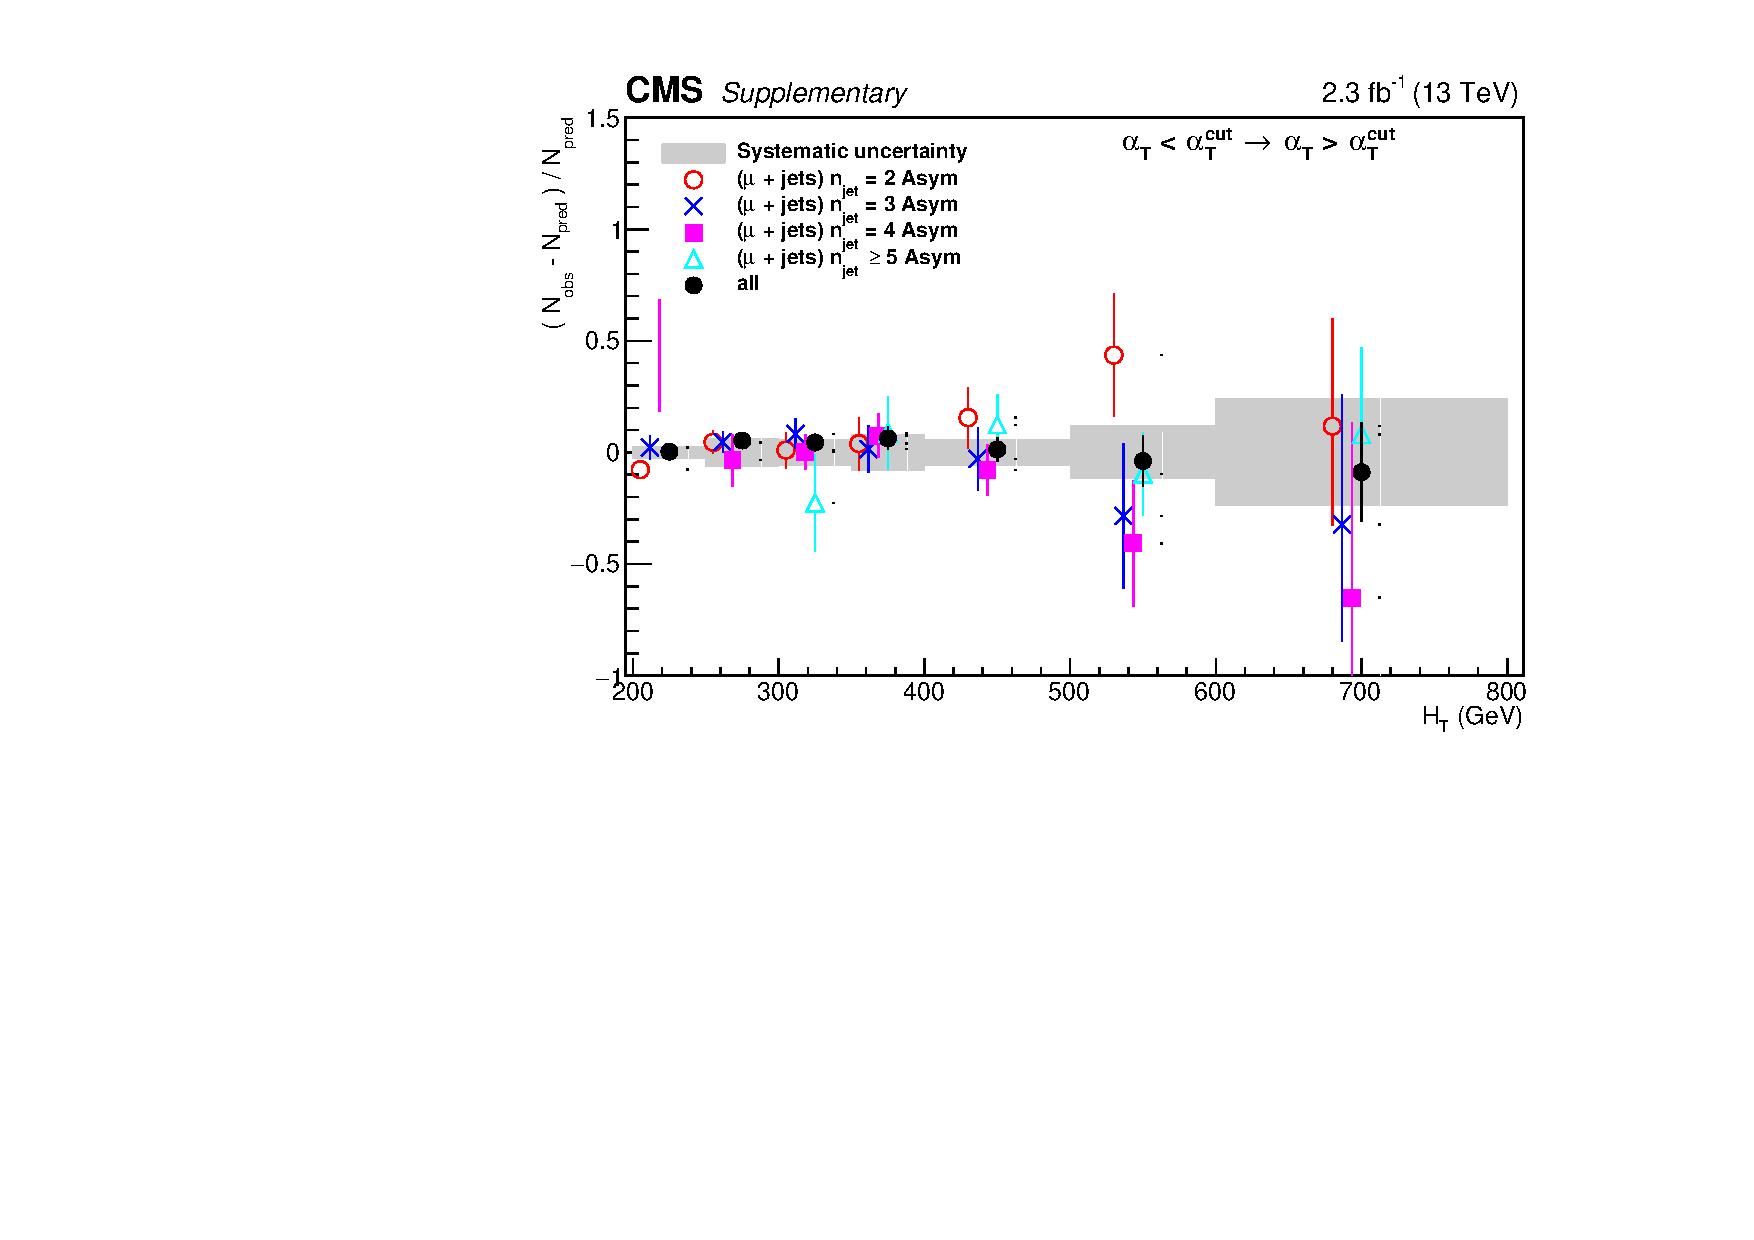
\includegraphics[width=0.48\textwidth]{figures/alphaTasym__noFit}
  \end{center}
\end{figure}

\begin{figure}[tbhp]
    \caption{ 
  Data-derived test of the modelling of the Z/W ratio for the symmetric (left) and asymmetric (right) jet categories. 
  In this test, the data yield in the \mmj sample ($N_{\mathrm{obs}}$) 
  is compared with the prediction obtained from the \mj sample multiplied by the corresponding 
  transfer factor computed in simulation ($N_{\mathrm{pred}}$). 
  A systematic uncertainty (grey band) is derived, as a function of \scalht and separately for symmetric and asymmetric categories, 
  to cover the non-closure. 
    \label{fig:CT-alphaT} }
  \begin{center}
     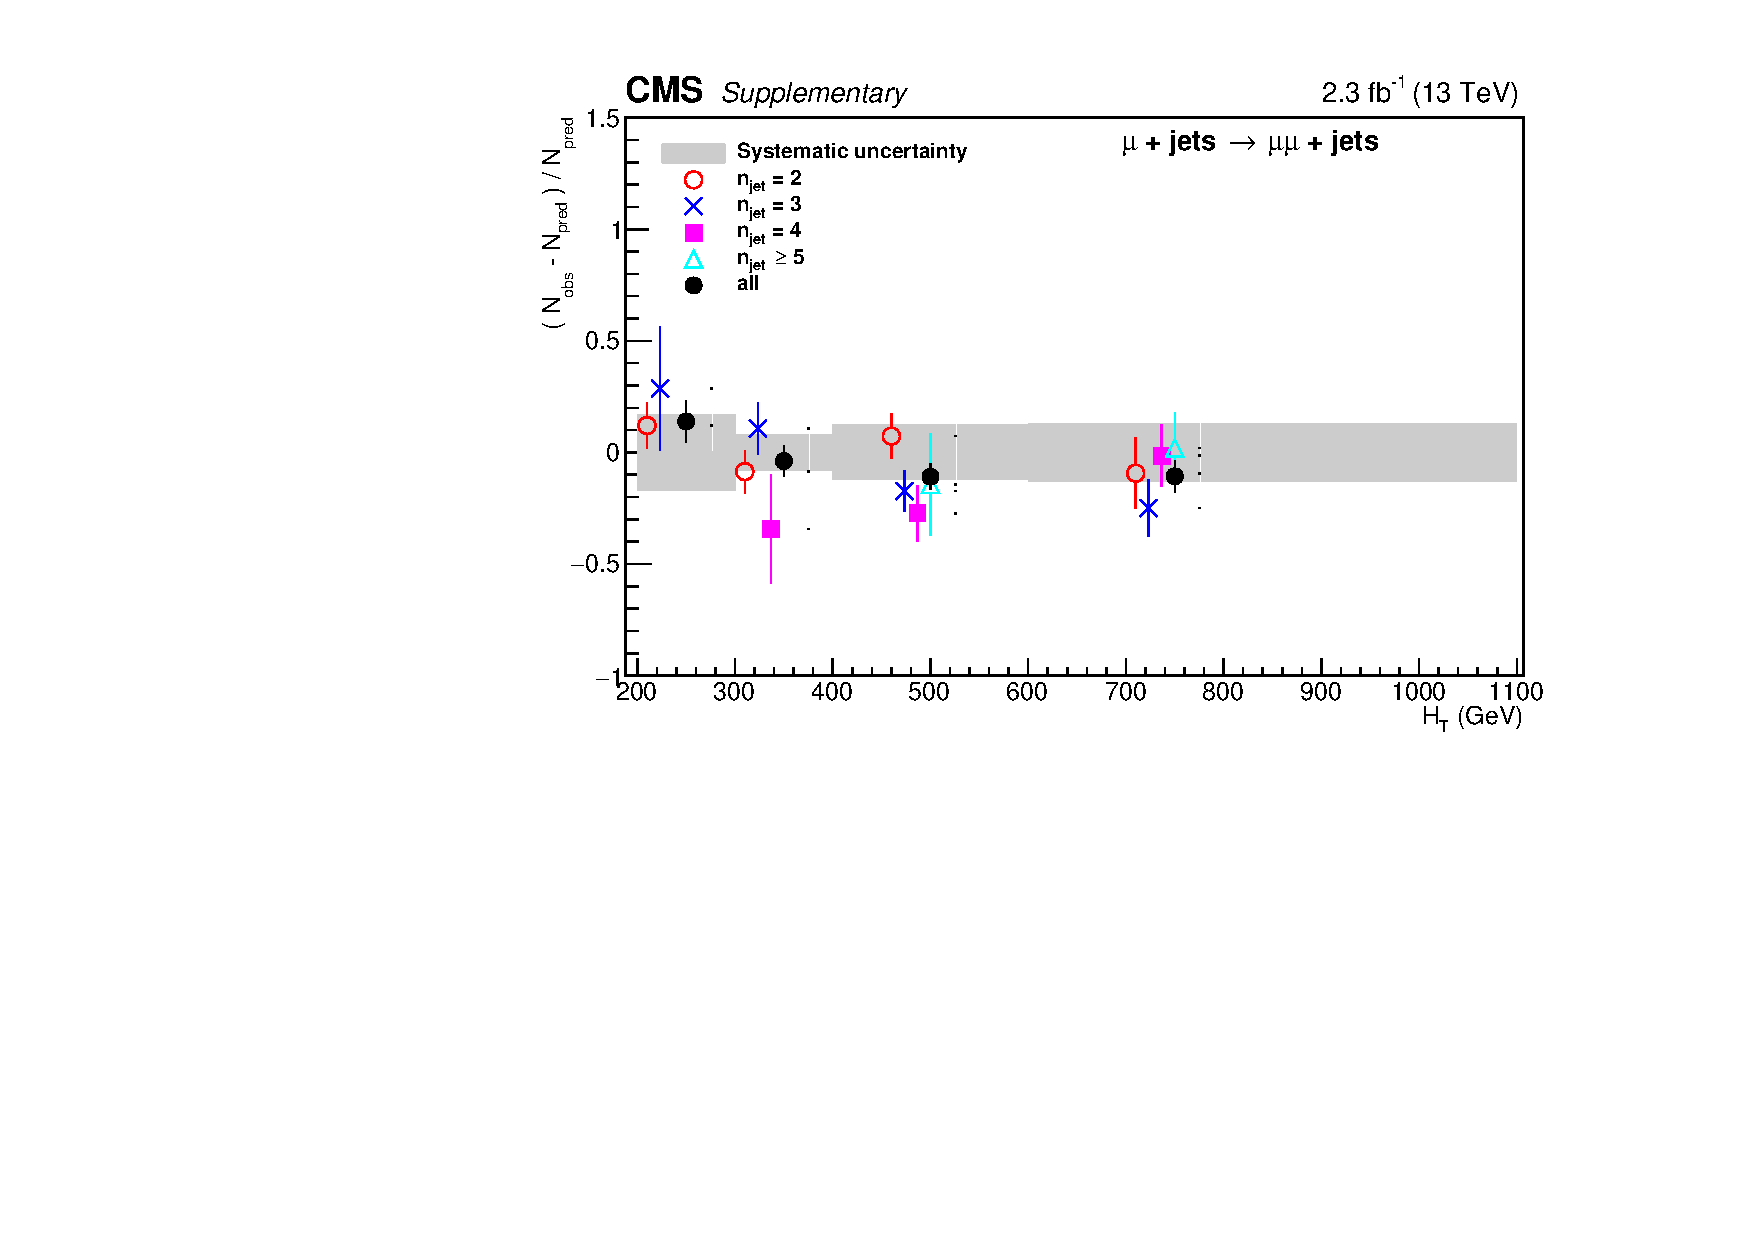
\includegraphics[width=0.48\textwidth]{figures/mu_mumusym_half_noFit} ~~
     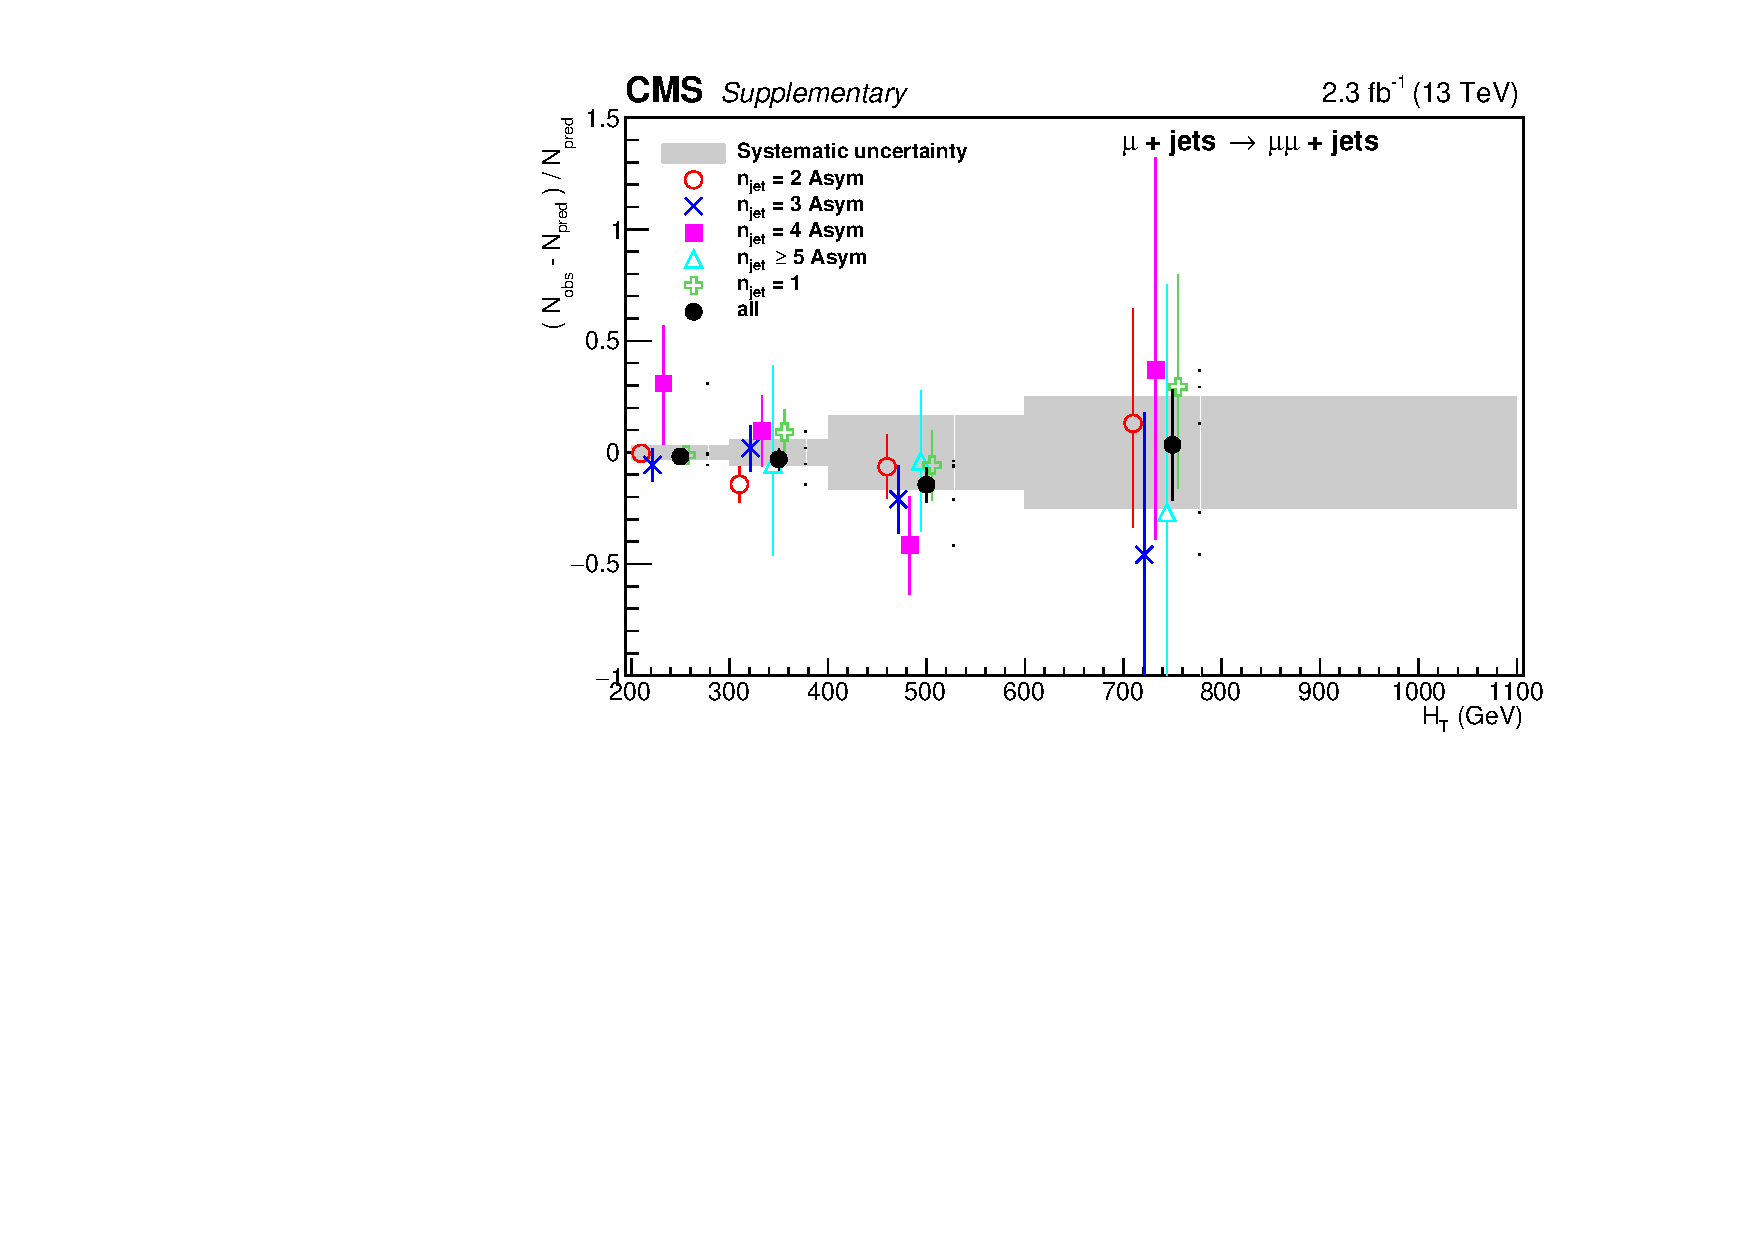
\includegraphics[width=0.48\textwidth]{figures/mu_mumuasym_half_noFit}
  \end{center}
\end{figure}





\clearpage
\begin{figure}[tbhp]
    \caption{ 
    Validation of the \mht modelling in the MC, in bins of (\nj,\nb,\scalht), for the $\gamma+\mathrm{jets}$ (top), $\mu+\mathrm{jets}$ (middle),             
    $\mu\mu+\mathrm{jets}$ (bottom) control regions. The data/MC ratio is fitted with constant and linear functions to spot for possible 
    trends and the result of these fits are shown in the plot. The best fit value of the linear function and its uncertainty are propagated 
    to assign shape systematic uncertainty in each (\nj,\nb,\scalht) category. 
    \label{fig:mht-validation} }
  \begin{center}
    \subfigure[$\gamma+\mathrm{jets}$, $\nj=2,\nb=0,600<\scalht<800 \, \mathrm{GeV}$]{ 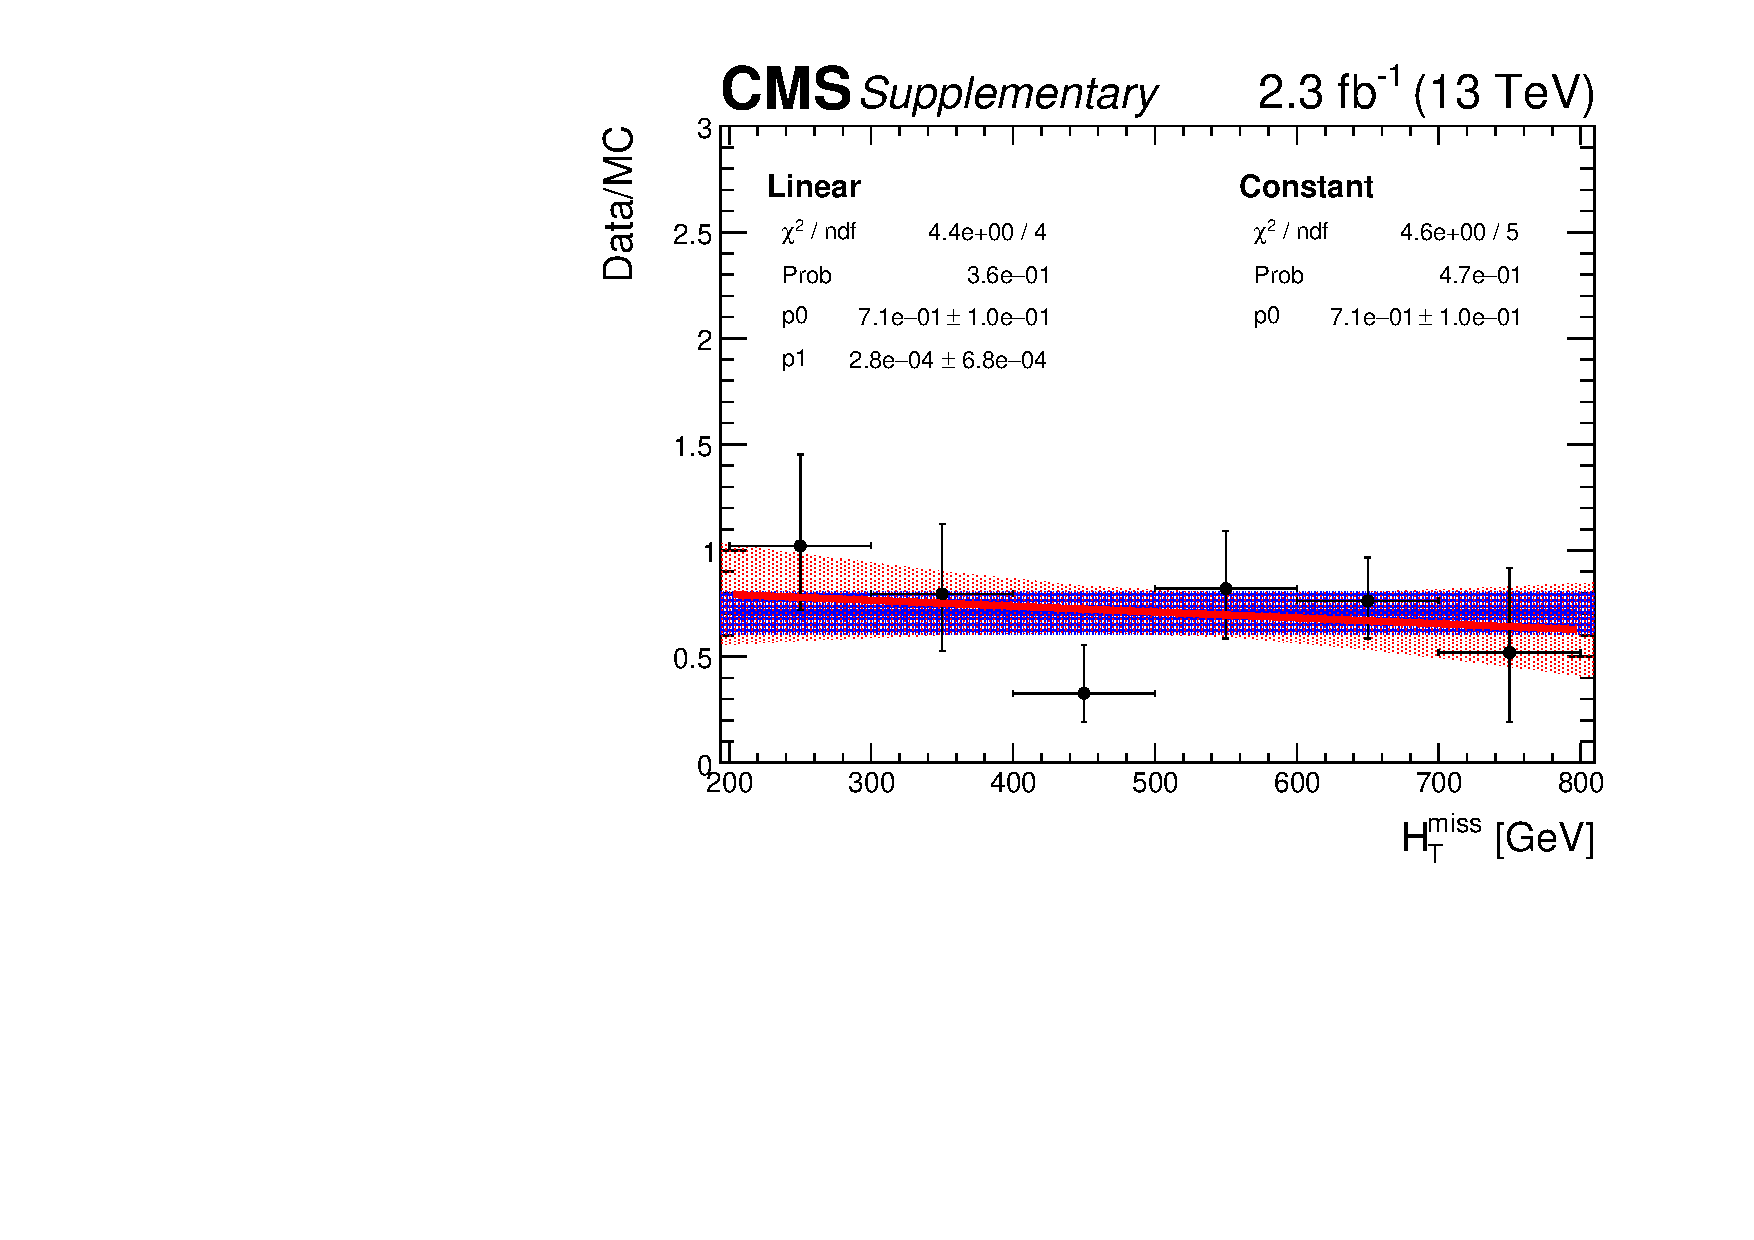
\includegraphics[width=0.45\textwidth]{figures/mht_eq0b_eq2j_ht_600_800_SinglePhoton_Graph} } ~~
    \subfigure[$\gamma+\mathrm{jets}$, $\nj=4,\nb=1,600<\scalht<800 \, \mathrm{GeV}$]{ 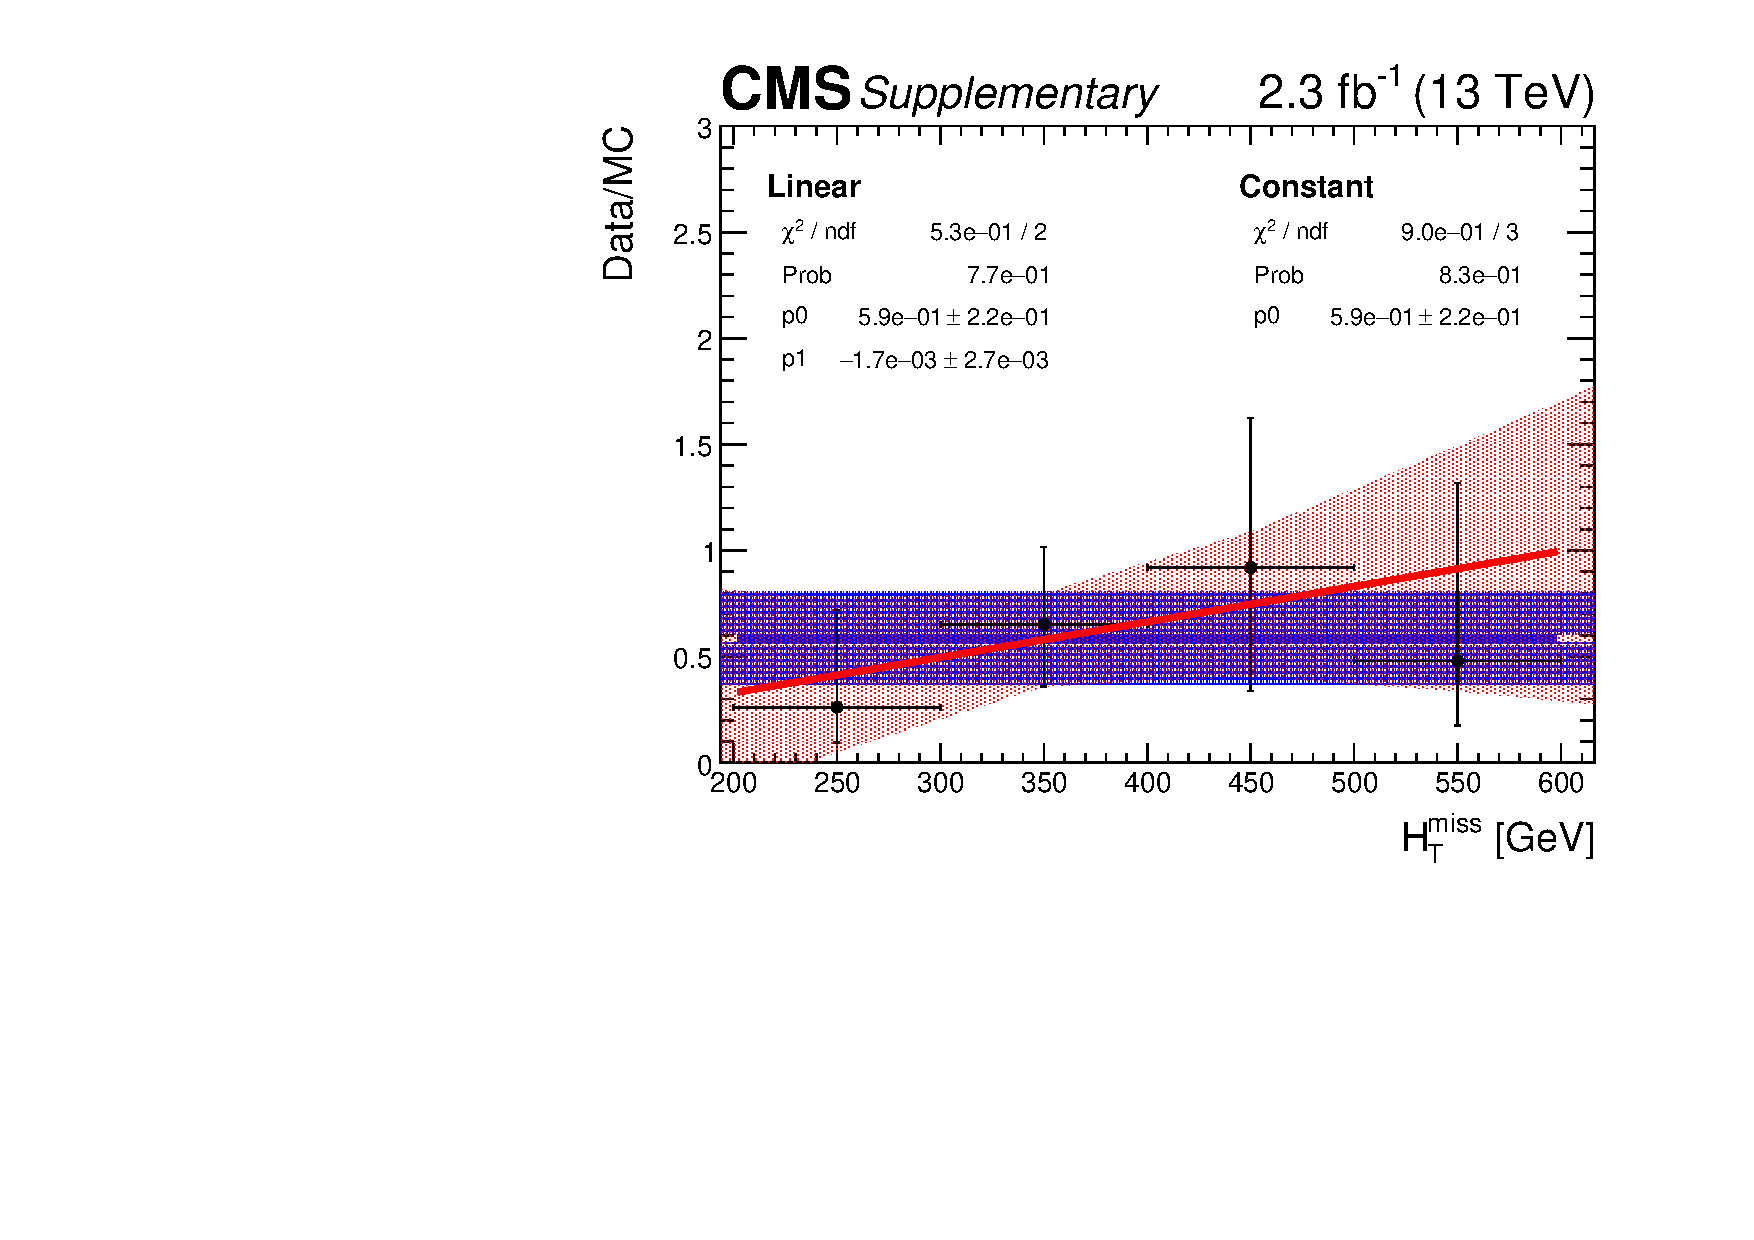
\includegraphics[width=0.45\textwidth]{figures/mht_eq1b_eq4j_ht_600_800_SinglePhoton_Graph} } \\
    \subfigure[$\mu+\mathrm{jets}$, $\nj^{asym}\geq5,\nb=2,350<\scalht<400 \, \mathrm{GeV}$]{ 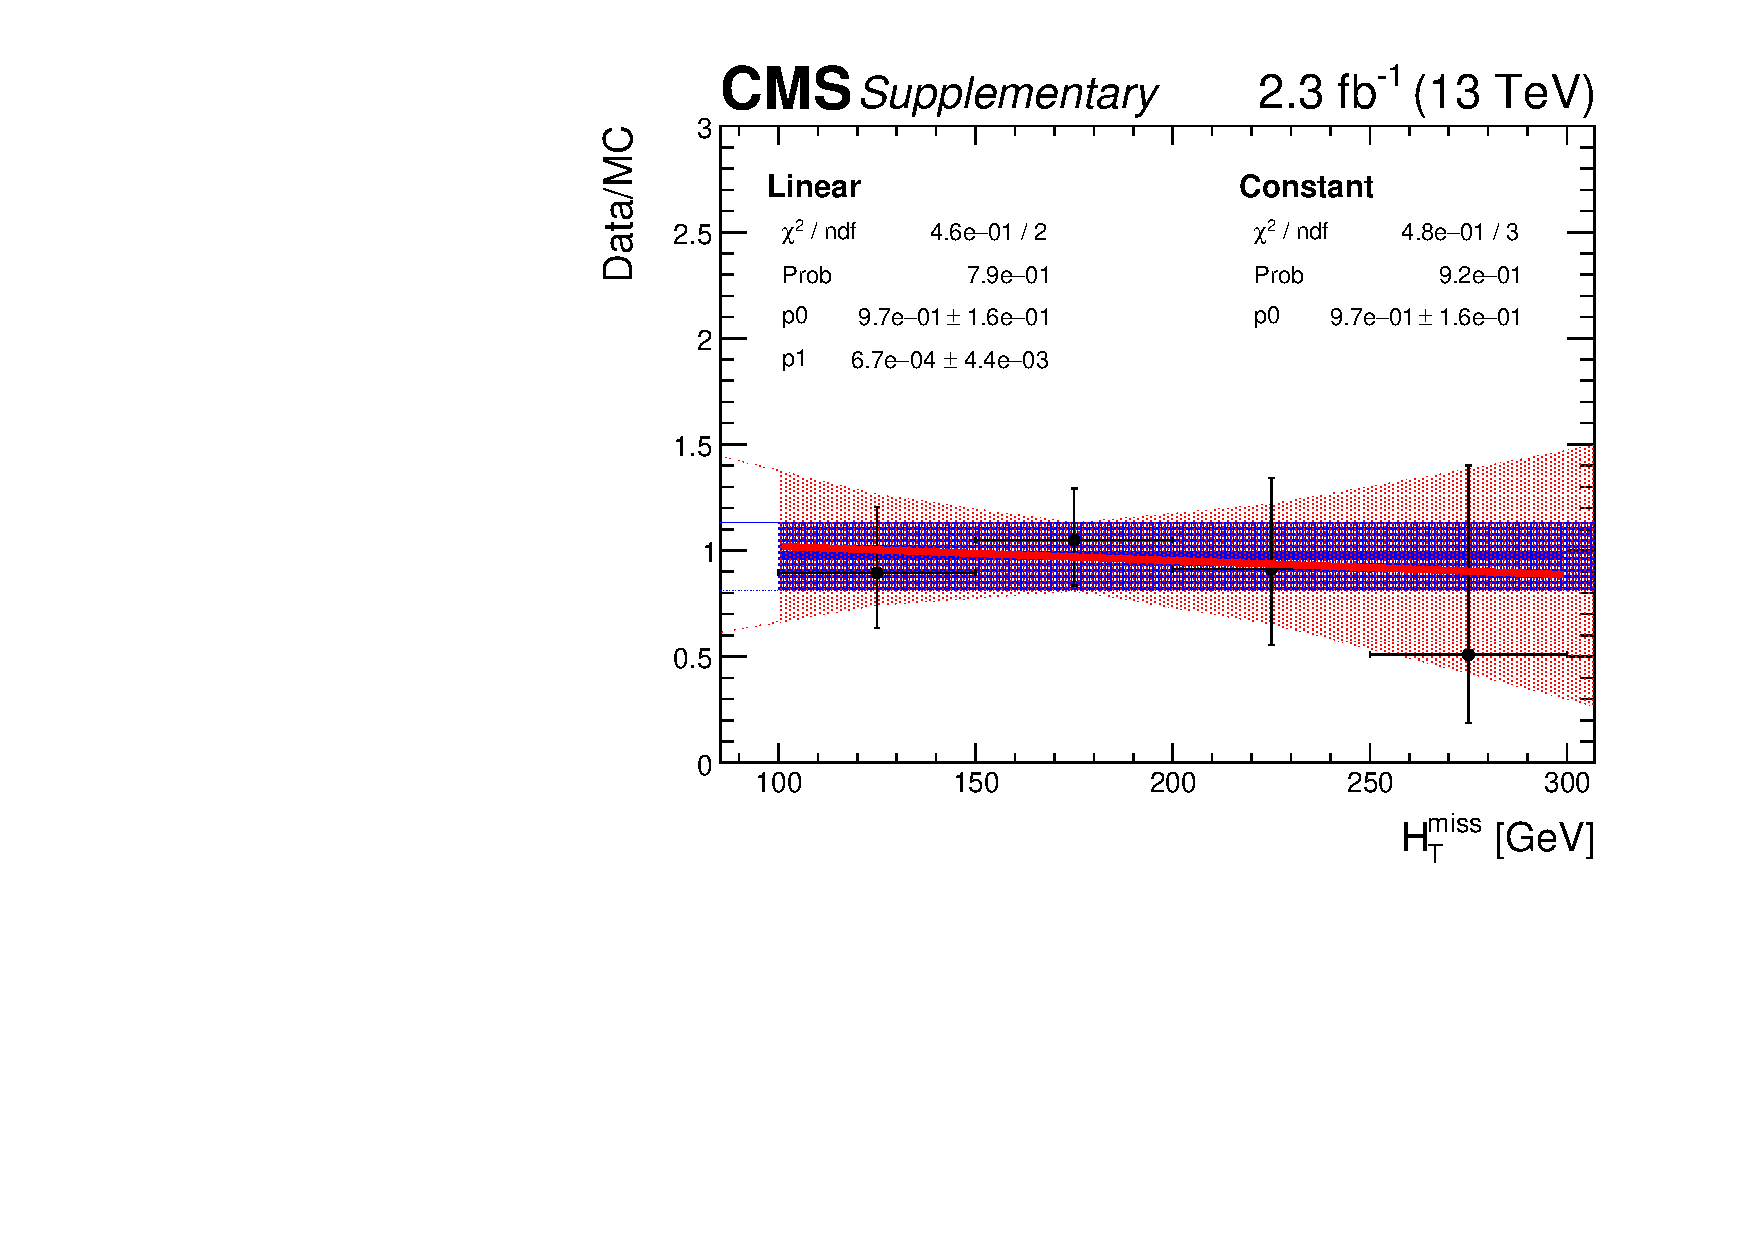
\includegraphics[width=0.45\textwidth]{figures/mht_eq2b_ge5a_ht_350_400_SingleMu_Graph} } ~~
    \subfigure[$\mu+\mathrm{jets}$, $\nj\geq5,\nb=0,\scalht>800 \, \mathrm{GeV}$]{ 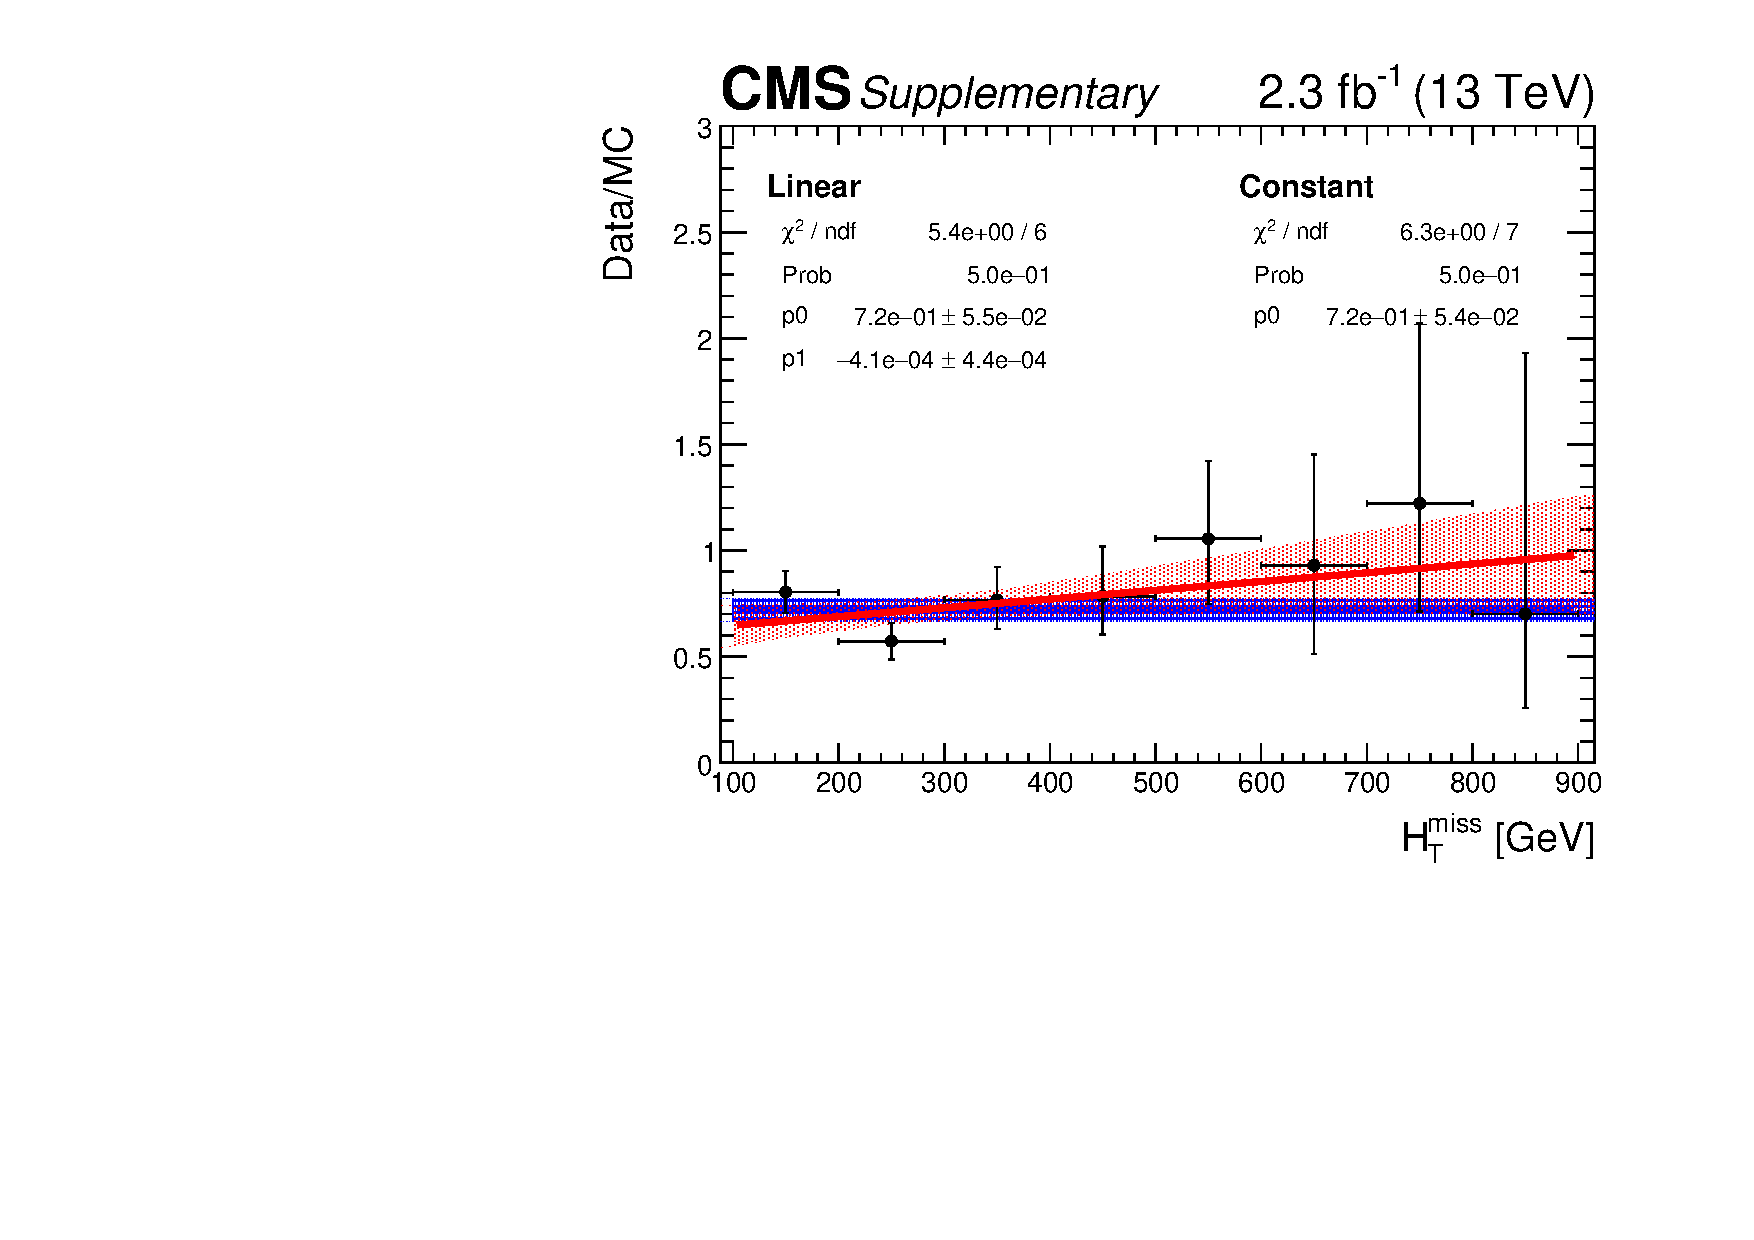
\includegraphics[width=0.45\textwidth]{figures/mht_eq0b_ge5j_ht_800_Inf_SingleMu_Graph} } \\
    \subfigure[$\mu\mu+\mathrm{jets}$, $\nj^{asym}=3,\nb=0,200<\scalht<250 \, \mathrm{GeV}$]{ 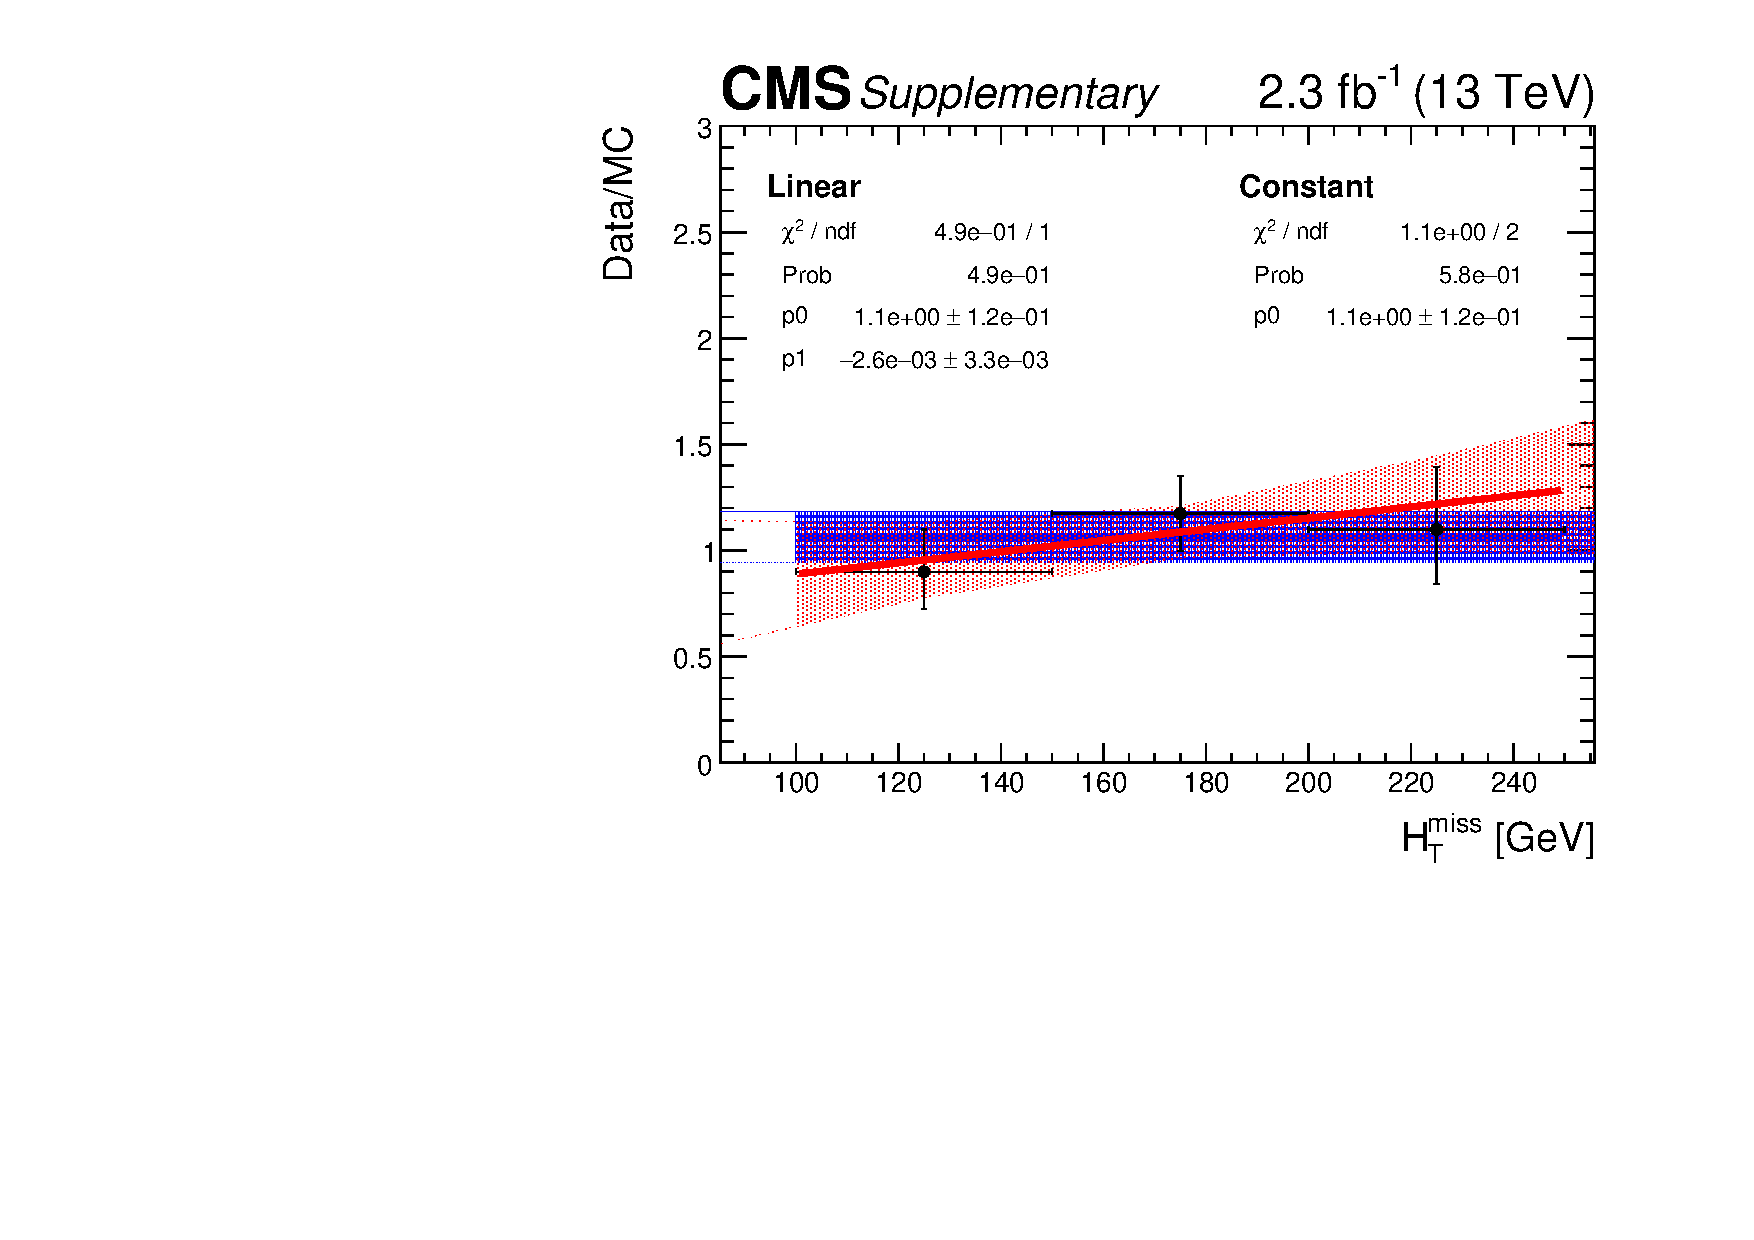
\includegraphics[width=0.45\textwidth]{figures/mht_eq0b_eq3a_ht_200_250_DoubleMu_Graph} } ~~
    \subfigure[$\mu\mu+\mathrm{jets}$, $\nj=2,\nb=0,400<\scalht<500 \, \mathrm{GeV}$]{ 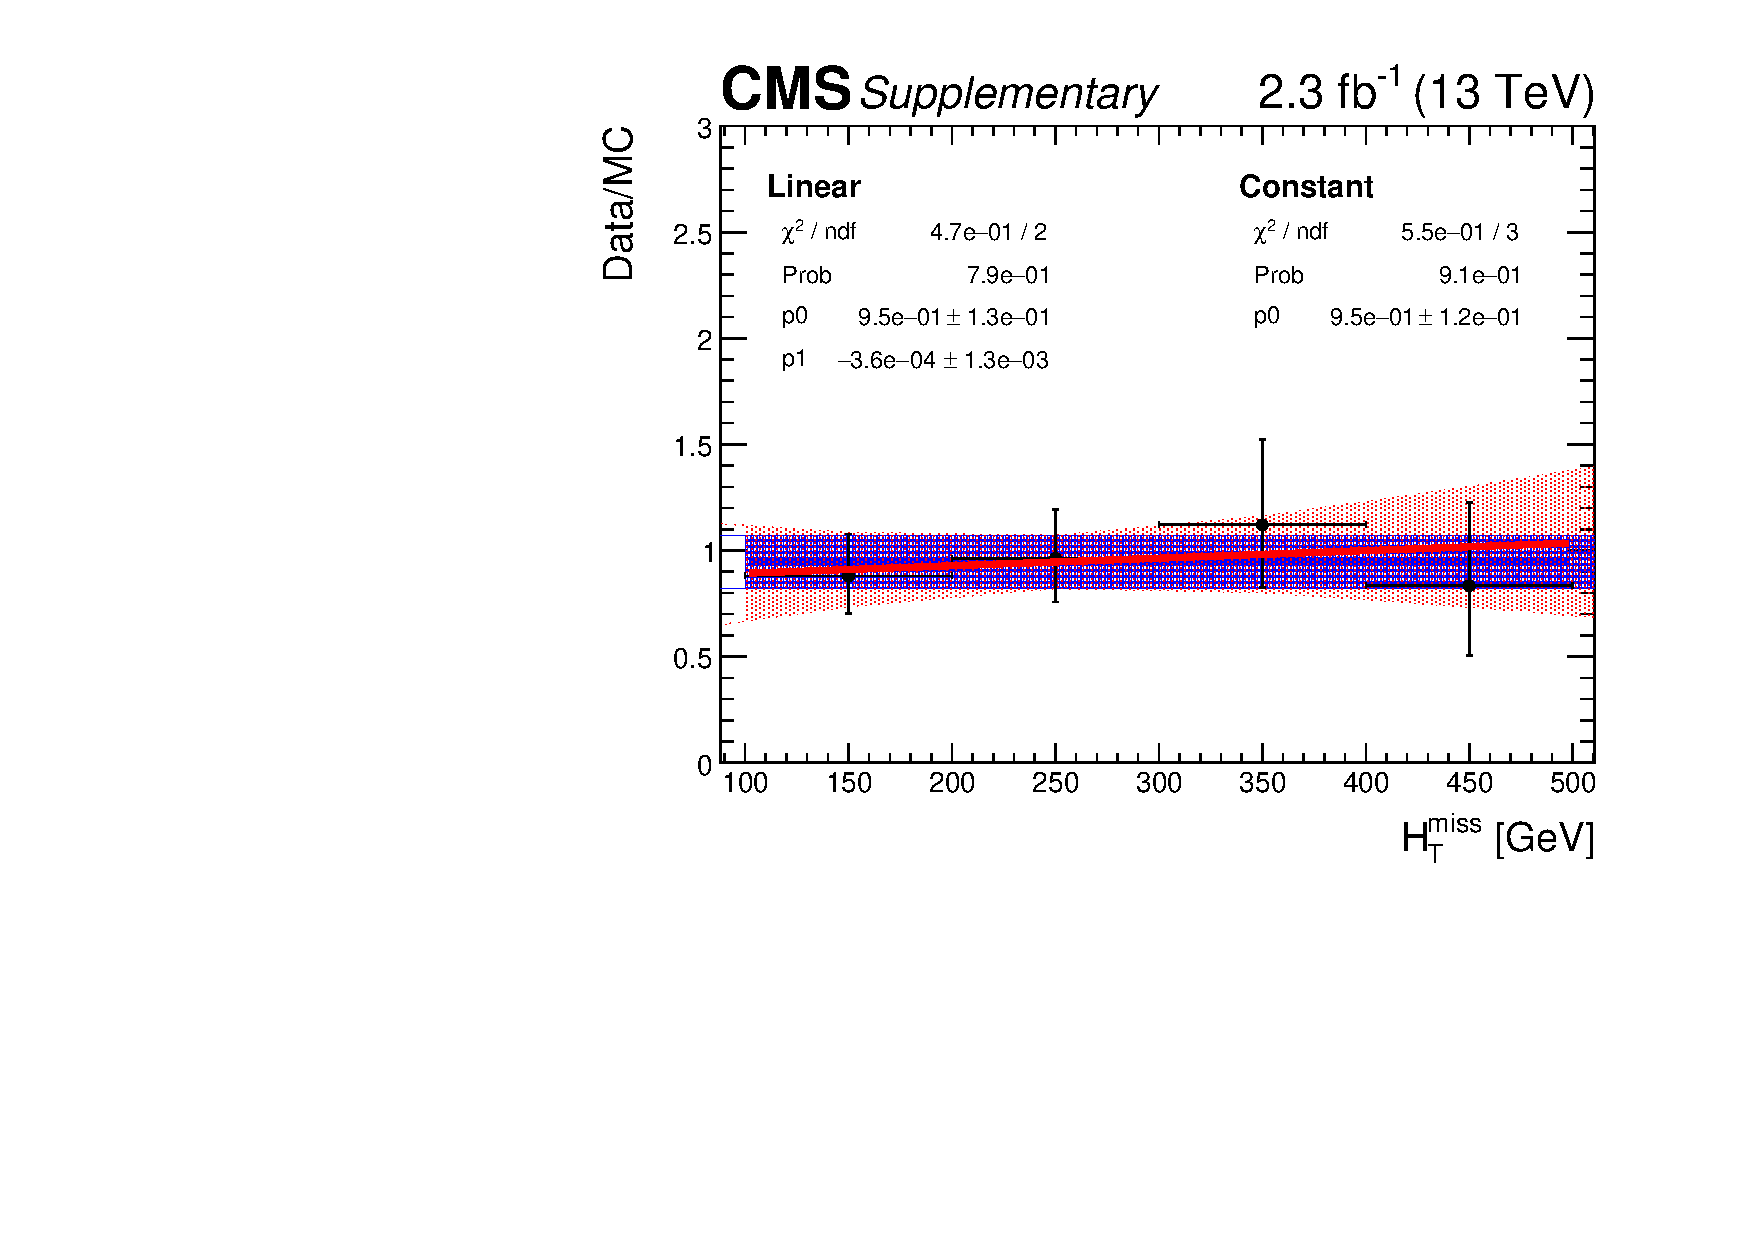
\includegraphics[width=0.45\textwidth]{figures/mht_eq0b_eq2j_ht_400_500_DoubleMu_Graph} } \\
  \end{center}
\end{figure}


%% \clearpage
%% \begin{landscape}
%% \begin{table}[h!]
%%   \caption{Summary of the systematics on the transfer factors considered in the analysis, 
%%     with representatives ranges of uncertainties and the correlation assumed, 
%%     for the predictions of the $\ttbar$, W and $\znunu$  background
%%     components.}
%%   \label{tab:systs}
%%   \centering
%%   \footnotesize
%%   \begin{tabular}{ ccccccc }
%%     \hline
%%     \hline
%%     Systematic & Method & \multicolumn{4}{c}{Relative uncertainty on transfer factor} & Correlation model \\    
%%      & & $\mj \rightarrow \znunu$  & $\mmj \rightarrow \znunu$ & $\gj \rightarrow \znunu$ & $\mj \rightarrow \ttbar+W$ & \\
%%     \hline
%%     \alphat/\bdphi extrapolation & data-driven tests & $5-80\%$ &
%%     $50-80\%$ & - & $5-80\%$ & un-correlated across \scalht/jet top. \\
%%     W/Z ratio & data-driven tests & $10-30\%$ & - & - & - & un-correlated across \scalht/jet top. \\
%%     Z/$\gamma$ ratio & data-driven tests & - & - & $10-30\%$ & - & un-correlated across \scalht/jet top. \\
%%     W/\ttbar admixture & data-driven tests & - & - & - & $10-100\%$ & un-correlated across \scalht/jet top. \\
%%     W polarisation & data-driven tests & $5-50\%$ & - & - & $5-50\%$ & un-correlated across \scalht/jet top. \\
%%     Jet energy scale & MC variations & $<15\%$ & $<10\%$ & $<15\%$ &
%%     $<15\%$ & fully correlated \\
%%     B-tagging efficiency & MC variations & $<5\%$ & $<2\%$ & $<2\%$
%%     & $<5\%$ & fully correlated \\
%%     Pileup weights & MC variations & $<6\%$ & $<4\%$ & $<3\%$ & $<10\%$ & fully correlated \\
%%     Top $p_{T}$ weights & MC variations & $<20\%$  & $<4\%$ & - &
%%     $<5\%$ & fully correlated \\
%%     Lepton selection & MC variations & - & - & - & $2-5\%$ & fully correlated \\
%%     \hline
%%     \hline
%%   \end{tabular}
%% \end{table}

%% \end{landscape}


%% \clearpage
%% \begin{landscape}
%%   \begin{center}
%%     \begin{figure*}[h!]
%%       \caption{Top: background yield predictions and data observation for the (\njet,\nb,\scalht) analysis bins (integrated over \mht) in the ``monojet'' search regions. Some benchmark signal models of gluino pair production are also shown, corresponding to ``compressed'' and ``uncompressed'' scenarios. Bottom: pre-fit and post-fit normalised pulls, defined as $(\mathrm{data}-\mathrm{SM total})/\sigma_{bkg}$, where $\sigma_{bkg}=\sqrt{\sigma^{2}_{syst.}+\sigma^{2}_{stat.}}$.  \label{fig:summaryPlot_Monojet}}.
%%       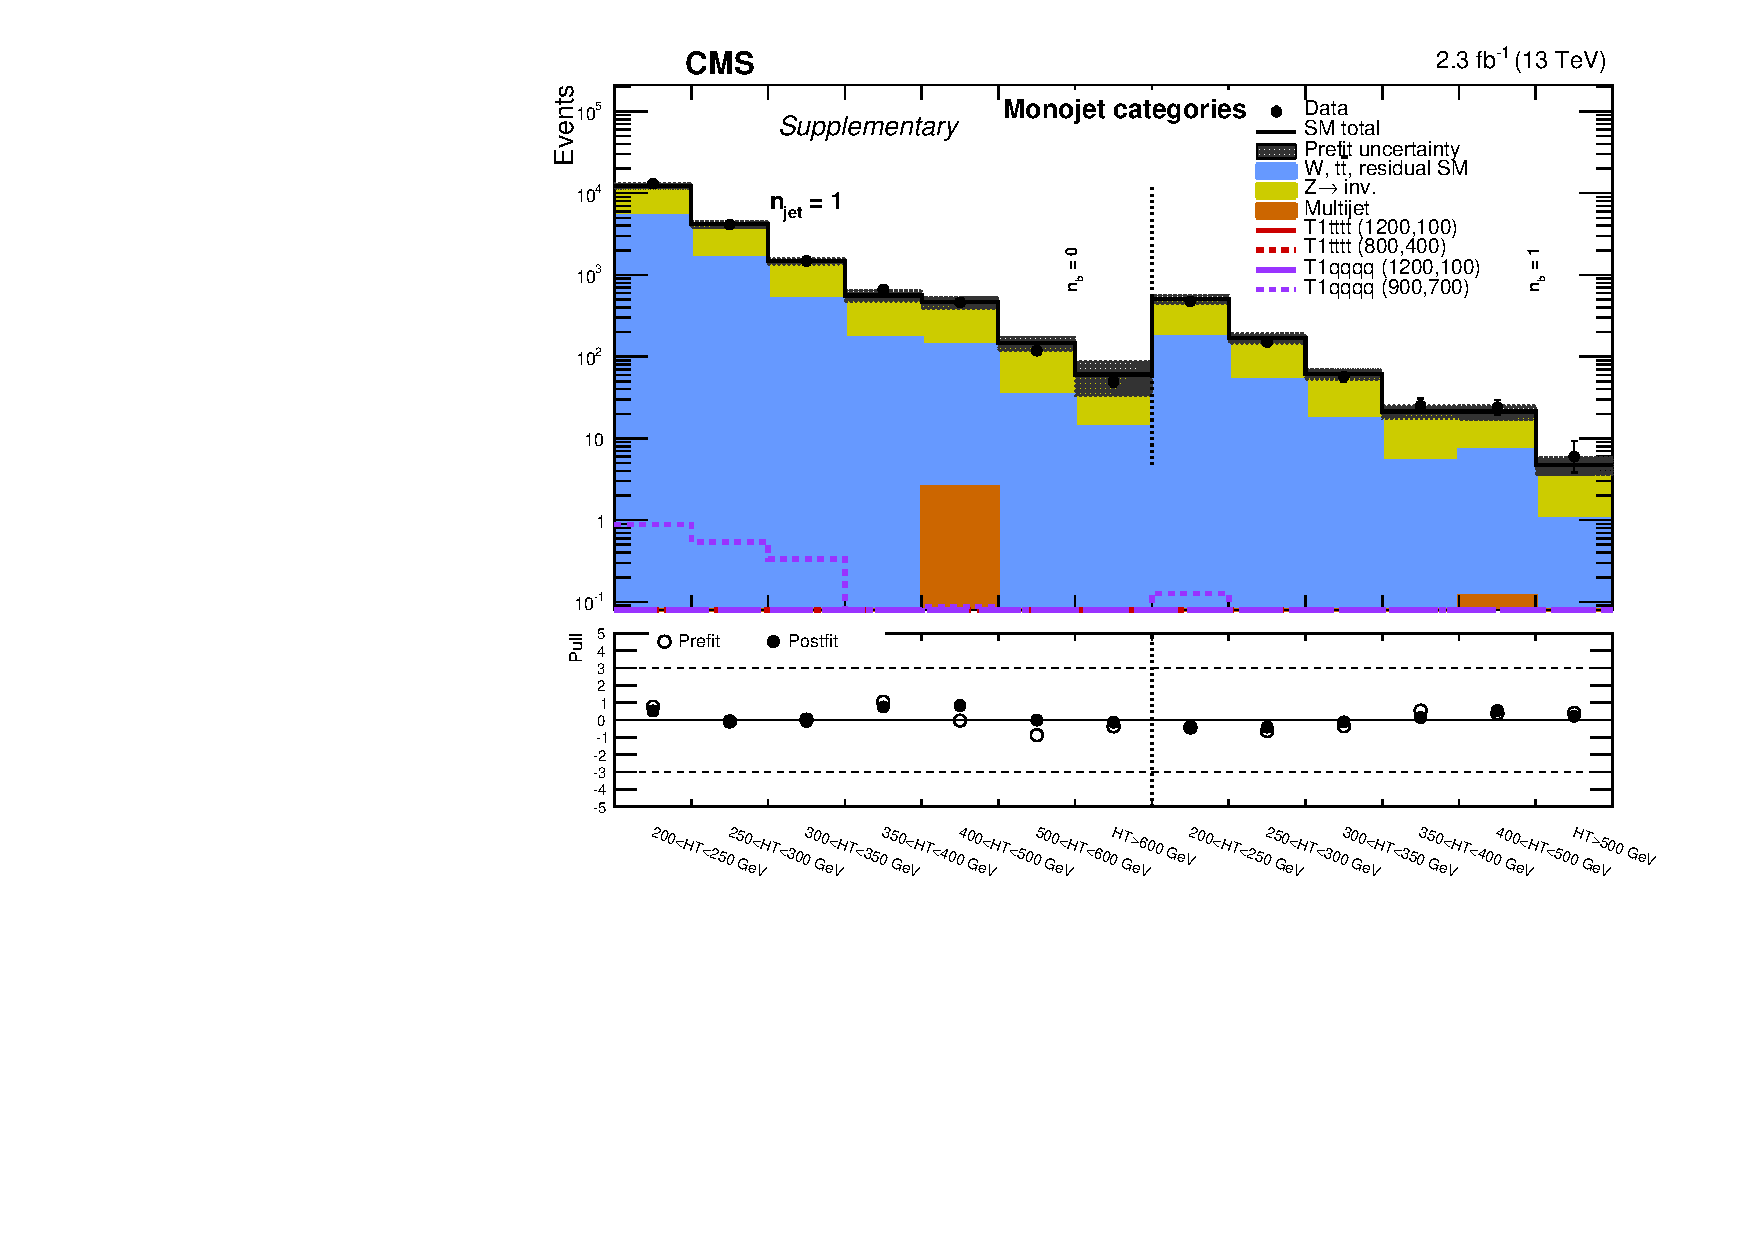
\includegraphics[width=0.75\linewidth]{supplementary/figures/summaryPlot_Monojet_prefit_overlay_fit_b}
%%     \end{figure*}
%%   \end{center}
%% \end{landscape}

%% \clearpage
%% \begin{landscape}
%%   \begin{center}
%%     \begin{figure*}[h!]
%%       \caption{Top: background yield predictions and data observation for the (\njet,\nb,\scalht) analysis bins (integrated over \mht) in the ``asymmetric'' search regions. Some benchmark signal models of gluino pair production are also shown, corresponding to ``compressed'' and ``uncompressed'' scenarios. Bottom: pre-fit and post-fit normalised pulls, defined as $(\mathrm{data}-\mathrm{SM total})/\sigma_{bkg}$, where $\sigma_{bkg}=\sqrt{\sigma^{2}_{syst.}+\sigma^{2}_{stat.}}$. \label{fig:summaryPlot_Asymmetric}}.
%%       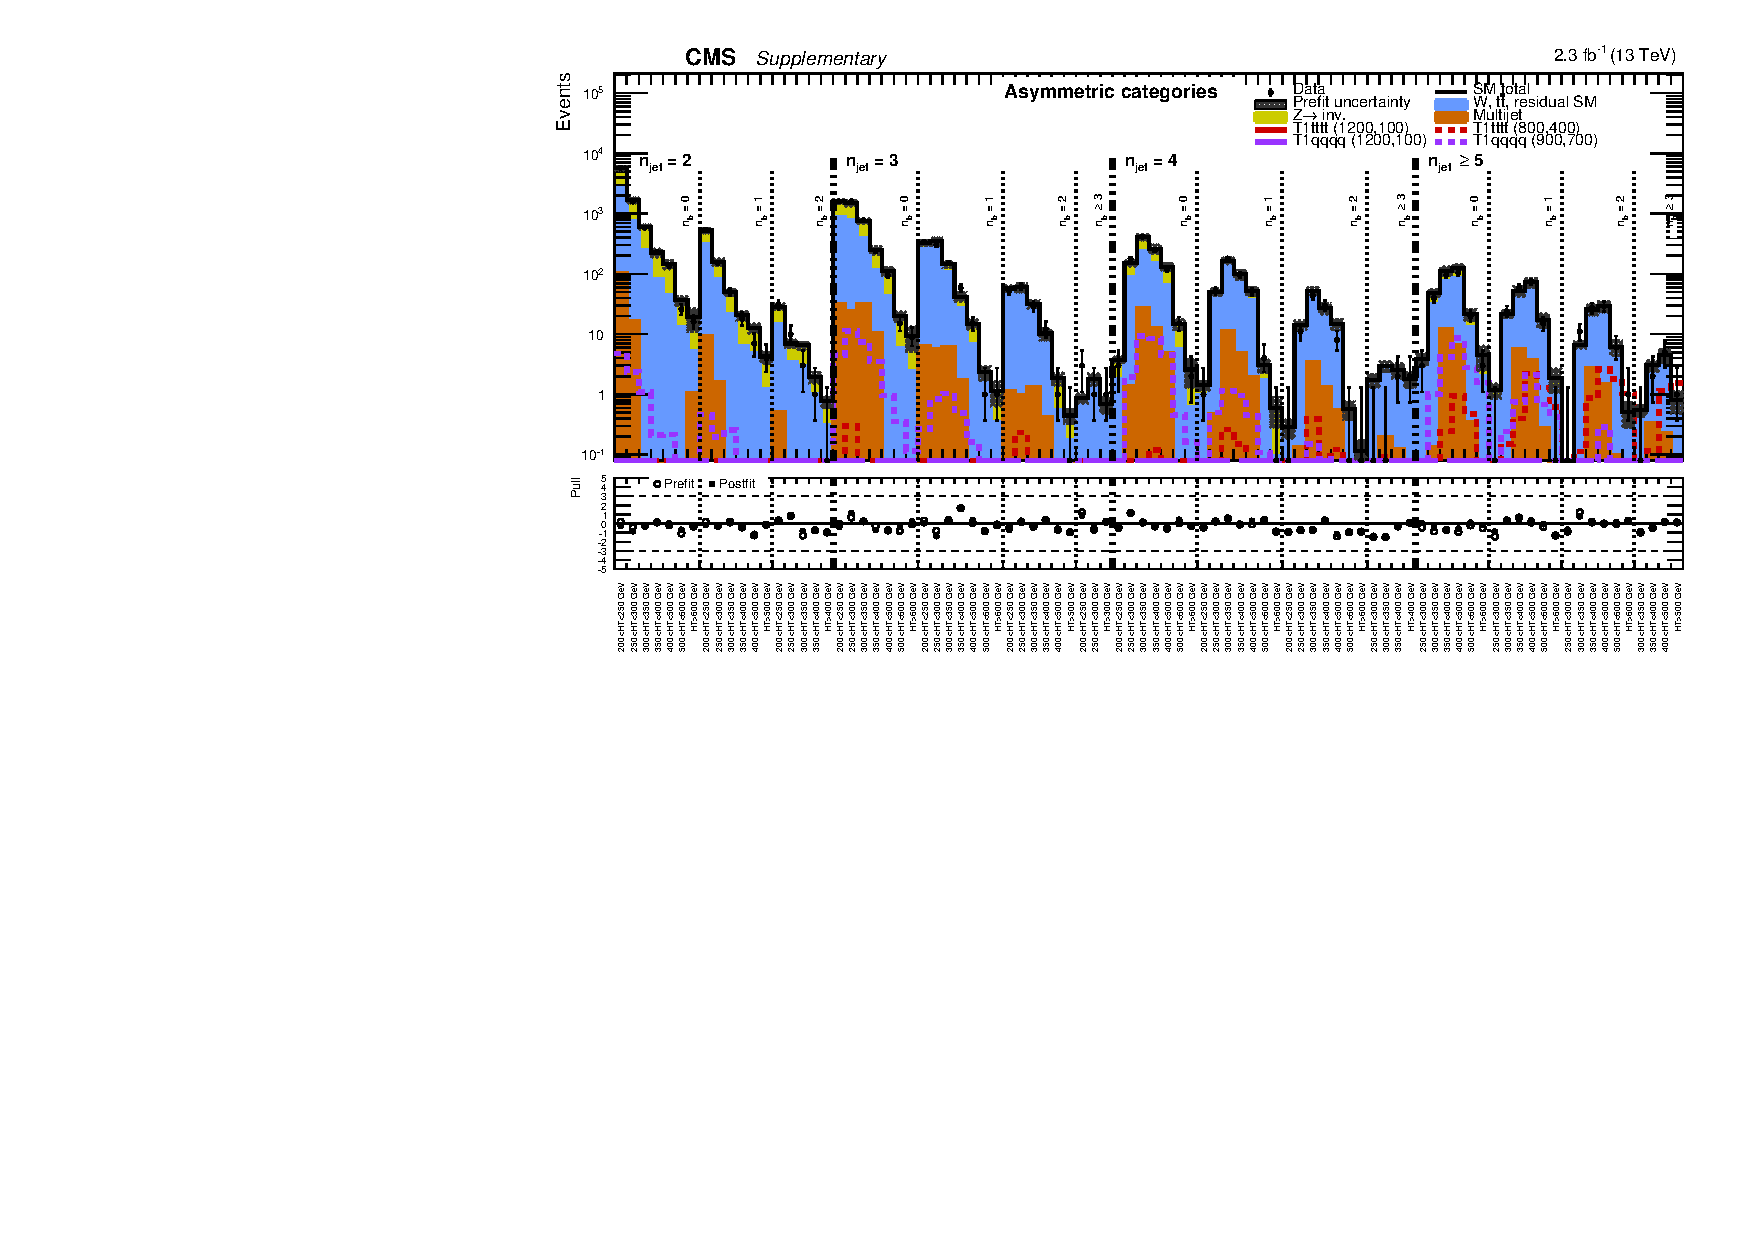
\includegraphics[width=0.8\linewidth]{supplementary/figures/summaryPlot_Asymmetric_prefit_overlay_fit_b}
%%     \end{figure*}
%%   \end{center}
%% \end{landscape}

%% \clearpage
%% \begin{landscape}
%%   \begin{center}
%%     \begin{figure*}[h!]
%%       \caption{Top: background yield predictions and data observation for the (\njet,\nb,\scalht) analysis bins (integrated over \mht) in the ``symmetric'' search regions. Some benchmark signal models of gluino pair production are also shown, corresponding to ``compressed'' and ``uncompressed'' scenarios. Bottom: pre-fit and post-fit normalised pulls, defined as $(\mathrm{data}-\mathrm{SM total})/\sigma_{bkg}$, where $\sigma_{bkg}=\sqrt{\sigma^{2}_{syst.}+\sigma^{2}_{stat.}}$. \label{fig:summaryPlot_Symmetric}}.
%%       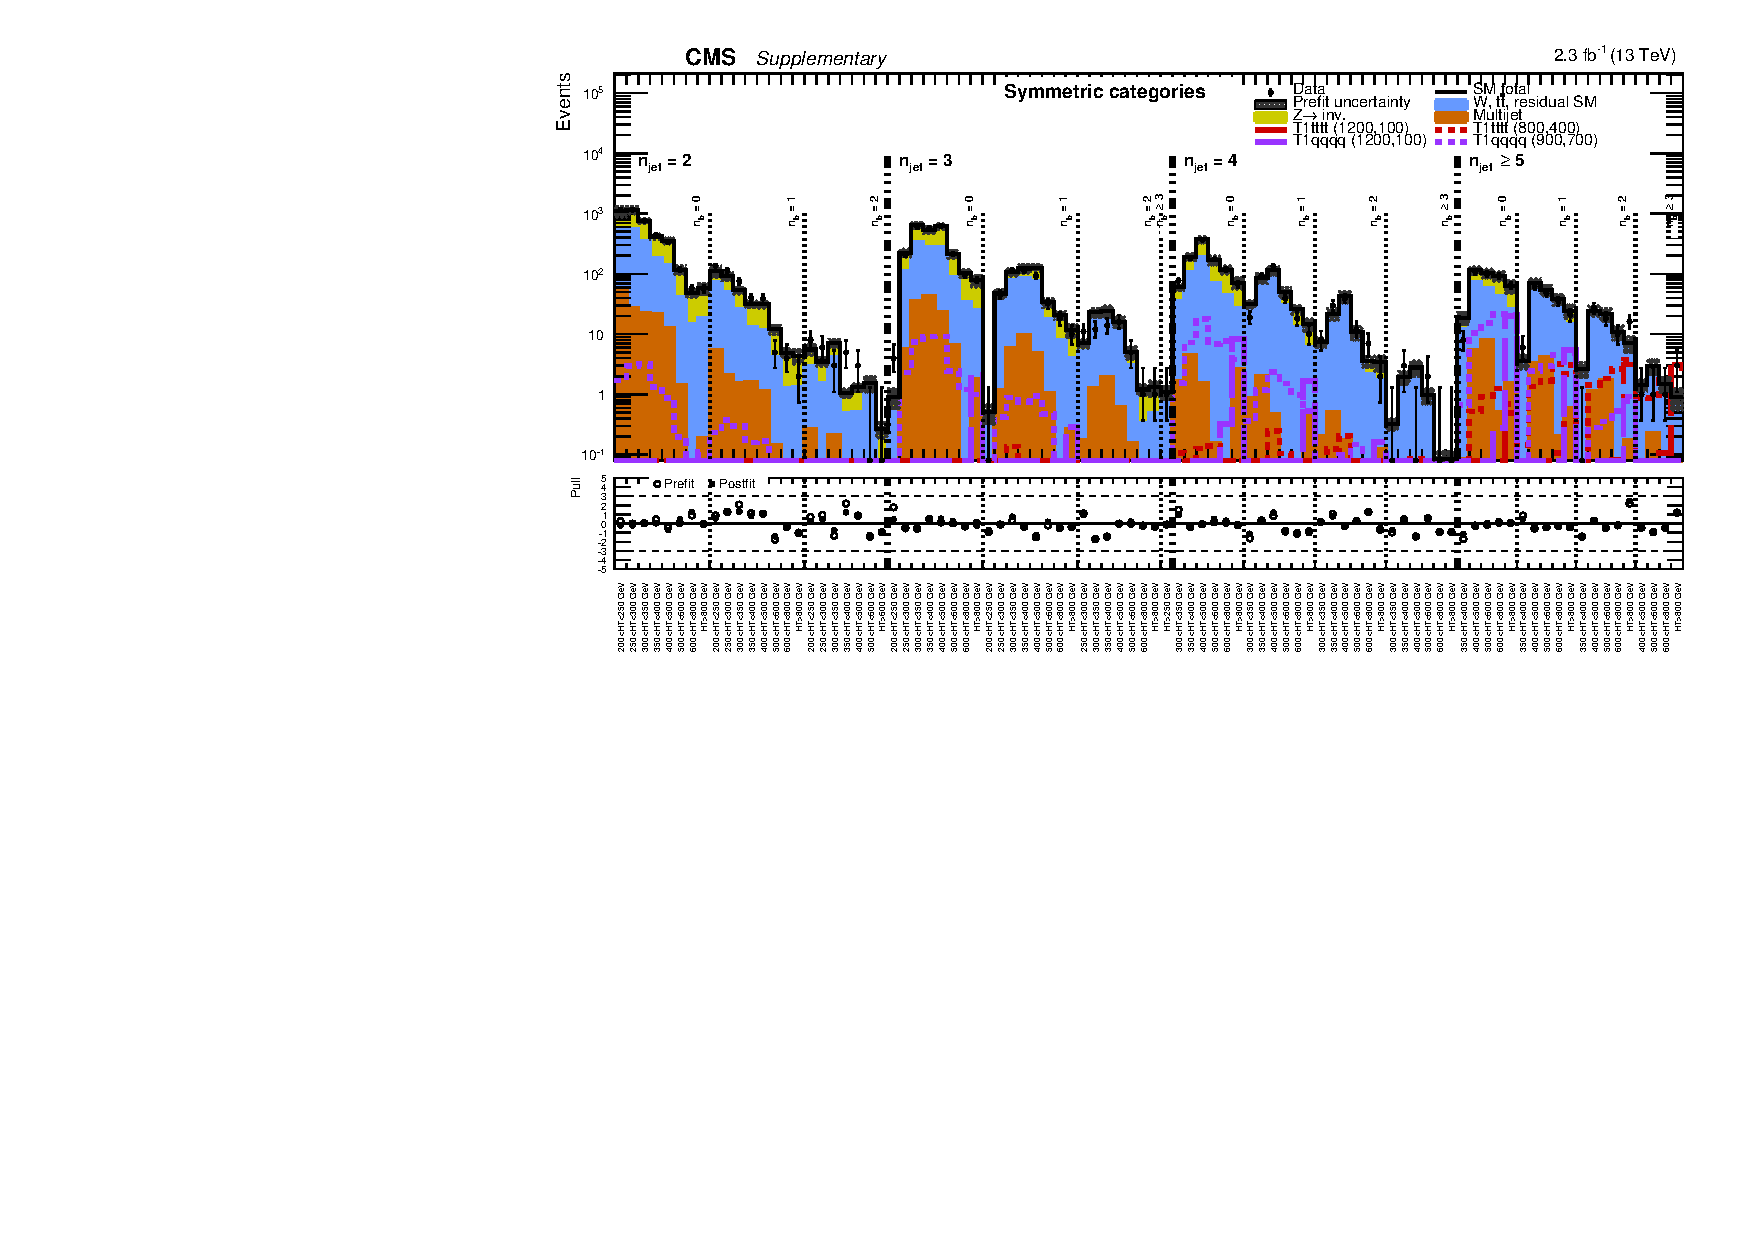
\includegraphics[width=0.8\linewidth]{supplementary/figures/summaryPlot_Symmetric_prefit_overlay_fit_b}
%%     \end{figure*}
%%   \end{center}
%% \end{landscape}


\clearpage
\begin{table}[h!]
\scriptsize
\centering
\caption{
  Observed data counts, ``pre-fit'' and ``post-fit'' background expectations  
  for all the \scalht bins and \njet, \nb multiplicity in the monojet event category. 
  The uncertainties include statistical as well as systematic contributions. 
  \label{tab:predewkdata_sig_comb_mono}}  
\scalebox{0.85}{\begin{tabular}{lccccccccc}
	\hline\hline
                    &              & \multicolumn{8}{c}{\scalht (\gev)}                                                                                                                                    \\ 
                    & (\njet, \nb) & 200-250               & 250-300              & 300-350              & 350-400            & 400-500            & 500-600            & 600-800           & 800-$\infty$ \\ [0.8ex] 
\hline
 Data & $(1j,0)$ & $13094$ & $4130$ & $1477$ & $663$ & $461$ & $118$ & $50$ & -- \\[0.5ex]
 SM pre-fit & $(1j,0)$ & $12319.3\pm985.8$ & $4167.9\pm384.1$ & $1474.1\pm155.2$ & $559.8\pm95.2$ & $463.1\pm74.5$ & $145.6\pm29.1$ & $60.4\pm25.1$ & -- \\[0.5ex]
 SM post-fit & $(1j,0)$ & $13012.3\pm112.8$ & $4133.5\pm57.7$ & $1480.8\pm33.9$ & $638.0\pm21.4$ & $439.5\pm16.0$ & $118.1\pm7.0$ & $51.3\pm6.4$ & -- \\[0.5ex]
 Data & $(1j,1)$ & $475$ & $151$ & $57$ & $25$ & $24$ & $6$ & -- & -- \\[0.5ex]
 SM pre-fit & $(1j,1)$ & $505.3\pm64.3$ & $169.6\pm24.6$ & $61.3\pm10.3$ & $21.3\pm4.5$ & $21.0\pm4.4$ & $4.7\pm1.3$ & -- & -- \\[0.5ex]
 SM post-fit & $(1j,1)$ & $488.4\pm18.1$ & $157.9\pm11.0$ & $58.1\pm6.2$ & $24.1\pm3.8$ & $20.8\pm2.6$ & $5.3\pm1.4$ & -- & -- \\[0.5ex]

	\hline
	\hline
\end{tabular}}
\end{table}


\clearpage
\begin{table}[h!]
\scriptsize
\centering
\caption{
  Observed data counts, ``pre-fit'' and ``post-fit'' background expectations  
  for all the \scalht bins and \njet, \nb multiplicity in the asymmetric event category. 
  The uncertainties include statistical as well as systematic contributions. 
  \label{tab:predewkdata_sig_comb_asym}}  
\scalebox{0.85}{\begin{tabular}{lccccccccc}
	\hline\hline
                    &                   & \multicolumn{8}{c}{\scalht (\gev)}                                                                                                                              \\ 
                    & (\njet, \nb)      & 200-250              & 250-300              & 300-350            & 350-400            & 400-500            & 500-600          & 600-800          & 800-$\infty$ \\ [0.8ex] 
\hline

 Data & $(2a,0)$ & $5788$ & $1585$ & $584$ & $232$ & $139$ & $26$ & $16$ & -- \\[0.5ex]
 SM pre-fit & $(2a,0)$ & $5890.6\pm544.0$ & $1695.0\pm180.5$ & $601.3\pm65.1$ & $224.3\pm38.4$ & $144.4\pm25.0$ & $36.4\pm7.1$ & $21.0\pm8.1$ & -- \\[0.5ex]
 SM post-fit & $(2a,0)$ & $5831.5\pm81.6$ & $1621.6\pm35.0$ & $581.0\pm17.9$ & $227.5\pm9.5$ & $136.5\pm6.4$ & $30.0\pm2.6$ & $18.3\pm3.2$ & -- \\[0.5ex]
 Data & $(2a,1)$ & $536$ & $152$ & $51$ & $18$ & $7$ & $4$ & -- & -- \\[0.5ex]
 SM pre-fit & $(2a,1)$ & $543.8\pm62.0$ & $161.7\pm22.6$ & $49.3\pm7.7$ & $20.5\pm3.9$ & $12.9\pm2.6$ & $4.3\pm1.0$ & -- & -- \\[0.5ex]
 SM post-fit & $(2a,1)$ & $541.0\pm16.4$ & $153.8\pm7.1$ & $49.7\pm3.7$ & $19.7\pm2.2$ & $10.7\pm1.4$ & $4.0\pm1.0$ & -- & -- \\[0.5ex]
 Data & $(2a,2)$ & $31$ & $10$ & $3$ & $1$ & $0$ & -- & -- & -- \\[0.5ex]
 SM pre-fit & $(2a,2)$ & $29.7\pm4.0$ & $7.2\pm1.2$ & $6.5\pm1.2$ & $2.0\pm0.5$ & $0.8\pm0.2$ & -- & -- & -- \\[0.5ex]
 SM post-fit & $(2a,2)$ & $29.5\pm3.5$ & $7.4\pm1.2$ & $5.0\pm1.1$ & $1.8\pm0.6$ & $0.6\pm0.3$ & -- & -- & -- \\[0.5ex]
 Data & $(3a,0)$ & $1599$ & $1609$ & $777$ & $239$ & $95$ & $15$ & $9$ & -- \\[0.5ex]
 SM pre-fit & $(3a,0)$ & $1669.4\pm163.3$ & $1529.4\pm171.2$ & $822.9\pm127.9$ & $272.3\pm60.5$ & $111.3\pm18.2$ & $19.7\pm4.0$ & $9.3\pm4.1$ & -- \\[0.5ex]
 SM post-fit & $(3a,0)$ & $1624.8\pm39.6$ & $1561.5\pm44.5$ & $781.7\pm28.8$ & $258.7\pm13.4$ & $100.9\pm5.4$ & $16.5\pm1.7$ & $8.0\pm1.5$ & -- \\[0.5ex]
 Data & $(3a,1)$ & $340$ & $299$ & $152$ & $59$ & $15$ & $1$ & $1$ & -- \\[0.5ex]
 SM pre-fit & $(3a,1)$ & $340.3\pm38.6$ & $357.2\pm51.6$ & $156.6\pm28.2$ & $46.1\pm12.0$ & $14.6\pm2.7$ & $2.3\pm0.7$ & $1.1\pm0.5$ & -- \\[0.5ex]
 SM post-fit & $(3a,1)$ & $340.7\pm12.6$ & $335.8\pm13.1$ & $148.6\pm7.9$ & $47.1\pm3.6$ & $13.0\pm1.4$ & $2.0\pm0.5$ & $1.0\pm0.4$ & -- \\[0.5ex]
 Data & $(3a,2)$ & $52$ & $62$ & $29$ & $12$ & $1$ & $0$ & -- & -- \\[0.5ex]
 SM pre-fit & $(3a,2)$ & $59.3\pm7.6$ & $61.9\pm10.1$ & $34.2\pm7.0$ & $11.2\pm3.2$ & $1.9\pm0.4$ & $0.4\pm0.1$ & -- & -- \\[0.5ex]
 SM post-fit & $(3a,2)$ & $58.3\pm4.6$ & $60.1\pm3.8$ & $31.3\pm2.7$ & $11.1\pm1.5$ & $1.5\pm0.4$ & $0.4\pm0.2$ & -- & -- \\[0.5ex]
 Data & $(3a,\geq 3)$ & $3$ & $1$ & $1$ & -- & -- & -- & -- & -- \\[0.5ex]
 SM pre-fit & $(3a,\geq 3)$ & $0.9\pm0.2$ & $1.9\pm0.4$ & $0.8\pm0.2$ & -- & -- & -- & -- & -- \\[0.5ex]
 SM post-fit & $(3a,\geq 3)$ & $1.3\pm0.5$ & $1.5\pm0.6$ & $0.8\pm0.4$ & -- & -- & -- & -- & -- \\[0.5ex]
 Data & $(4a,0)$ & $3$ & $178$ & $412$ & $246$ & $119$ & $15$ & $2$ & -- \\[0.5ex]
 SM pre-fit & $(4a,0)$ & $3.8\pm0.5$ & $153.4\pm18.5$ & $462.8\pm89.5$ & $285.1\pm64.1$ & $142.4\pm22.6$ & $14.7\pm3.2$ & $2.6\pm1.2$ & -- \\[0.5ex]
 SM post-fit & $(4a,0)$ & $4.1\pm1.0$ & $159.3\pm10.8$ & $418.0\pm19.5$ & $256.7\pm14.2$ & $128.0\pm7.6$ & $12.9\pm1.7$ & $2.2\pm0.6$ & -- \\[0.5ex]
 Data & $(4a,1)$ & $1$ & $53$ & $180$ & $96$ & $51$ & $4$ & $0$ & -- \\[0.5ex]
 SM pre-fit & $(4a,1)$ & $1.4\pm0.3$ & $51.5\pm7.5$ & $189.7\pm39.6$ & $108.1\pm25.9$ & $55.6\pm10.1$ & $3.1\pm0.8$ & $0.6\pm0.3$ & -- \\[0.5ex]
 SM post-fit & $(4a,1)$ & $1.6\pm0.5$ & $50.7\pm4.6$ & $172.6\pm9.2$ & $98.9\pm6.8$ & $49.0\pm3.9$ & $2.9\pm0.6$ & $0.5\pm0.1$ & -- \\[0.5ex]
 Data & $(4a,2)$ & $0$ & $11$ & $44$ & $30$ & $8$ & $0$ & $0$ & -- \\[0.5ex]
 SM pre-fit & $(4a,2)$ & $0.3\pm0.1$ & $14.6\pm2.4$ & $58.5\pm12.8$ & $30.0\pm7.8$ & $15.6\pm3.3$ & $0.6\pm0.2$ & $0.1\pm0.1$ & -- \\[0.5ex]
 SM post-fit & $(4a,2)$ & $0.3\pm0.2$ & $13.9\pm1.5$ & $51.6\pm4.3$ & $28.7\pm2.9$ & $12.7\pm1.6$ & $0.6\pm0.2$ & $0.1\pm0.0$ & -- \\[0.5ex]
 Data & $(4a,\geq 3)$ & -- & $0$ & $0$ & $2$ & $2$ & -- & -- & -- \\[0.5ex]
 SM pre-fit & $(4a,\geq 3)$ & -- & $1.8\pm0.4$ & $3.2\pm0.8$ & $2.8\pm0.8$ & $1.9\pm0.5$ & -- & -- & -- \\[0.5ex]
 SM post-fit & $(4a,\geq 3)$ & -- & $1.3\pm0.5$ & $2.4\pm0.8$ & $2.3\pm0.7$ & $2.1\pm0.6$ & -- & -- & -- \\[0.5ex]
 Data & $(\geq 5a,0)$ & -- & $3$ & $40$ & $96$ & $105$ & $20$ & $3$ & -- \\[0.5ex]
 SM pre-fit & $(\geq 5a,0)$ & -- & $3.9\pm1.1$ & $49.2\pm8.4$ & $137.6\pm40.4$ & $138.2\pm25.5$ & $22.0\pm5.1$ & $4.5\pm2.0$ & -- \\[0.5ex]
 SM post-fit & $(\geq 5a,0)$ & -- & $2.9\pm1.3$ & $43.5\pm4.7$ & $107.8\pm8.9$ & $114.4\pm8.6$ & $19.6\pm2.6$ & $3.3\pm0.9$ & -- \\[0.5ex]
 Data & $(\geq 5a,1)$ & -- & $0$ & $24$ & $60$ & $74$ & $15$ & $0$ & -- \\[0.5ex]
 SM pre-fit & $(\geq 5a,1)$ & -- & $1.2\pm0.4$ & $22.0\pm3.9$ & $64.5\pm20.4$ & $80.0\pm16.7$ & $17.9\pm4.8$ & $1.9\pm0.9$ & -- \\[0.5ex]
 SM post-fit & $(\geq 5a,1)$ & -- & $0.8\pm0.5$ & $22.2\pm3.0$ & $57.4\pm5.9$ & $71.9\pm5.7$ & $15.4\pm2.3$ & $1.4\pm0.5$ & -- \\[0.5ex]
 Data & $(\geq 5a,2)$ & -- & $0$ & $11$ & $27$ & $29$ & $6$ & $1$ & -- \\[0.5ex]
 SM pre-fit & $(\geq 5a,2)$ & -- & $0.0\pm0.0$ & $6.8\pm1.3$ & $31.7\pm9.8$ & $32.1\pm7.1$ & $6.3\pm1.9$ & $0.5\pm0.3$ & -- \\[0.5ex]
 SM post-fit & $(\geq 5a,2)$ & -- & $0.0\pm0.0$ & $7.9\pm1.7$ & $27.3\pm3.3$ & $28.9\pm3.3$ & $5.5\pm1.2$ & $0.4\pm0.2$ & -- \\[0.5ex]
 Data & $(\geq 5a,\geq 3)$ & -- & -- & $0$ & $2$ & $5$ & $1$ & -- & -- \\[0.5ex]
 SM pre-fit & $(\geq 5a,\geq 3)$ & -- & -- & $0.5\pm0.1$ & $3.6\pm1.1$ & $5.0\pm1.3$ & $0.8\pm0.3$ & -- & -- \\[0.5ex]
 SM post-fit & $(\geq 5a,\geq 3)$ & -- & -- & $0.5\pm0.3$ & $3.0\pm0.9$ & $4.5\pm1.1$ & $0.9\pm0.4$ & -- & -- \\[0.5ex]



	\hline
	\hline
\end{tabular}}
\end{table}


\clearpage
{\begin{table}[h!]
\scriptsize
\centering
\caption{%CMS {\it Preliminary}, $\mathcal{L}_{\mathrm{int}} =
  %2.2\fbinv$, $\sqrt{s} = 13\TeV$. 
  %\newline
  Observed data counts and ``post-fit'' background expectations  
  based on the result of a combined fit to the signal region and multiple
  control regions under the SM-only hypothesis for the ``symmetric''
  event categories. The rows labelled SM ``pre-fit'' show the
  background expectations when excluding the signal region from the
  fit. The uncertainties include statistical as well as systematic
  contributions. 
  \label{tab:predewkdata_sig_comb_sym}}  
\scalebox{0.85}{\begin{tabular}{lccccccccc}
    \hline\hline
                &                  & \multicolumn{8}{c}{\scalht (\gev)}                                                                                                                                    \\ 
                & (\njet, \nb)     & 200-250             & 250-300             & 300-350            & 350-400            & 400-500            & 500-600            & 600-800           & 800-$\infty$      \\ [0.8ex] 
    \hline
    Data        & (2, 0)           & 968                 & 997                 & 657                & 398                & 301                & 110                & 56                & 49                \\[0.5ex] 
    SM post-fit & (2, 0)           & $969.9\pm{ 51.2 }$  & $996.4\pm{ 36.2 }$  & $656.8\pm{ 25.1 }$ & $395.5\pm{ 18.7 }$ & $312.3\pm{ 16.4 }$ & $107.3\pm{ 10.6 }$ & $53.1\pm{ 6.2 }$  & $47.2\pm{ 6.4 }$  \\[0.5ex] 
    SM pre-fit  & (2, 0)           & $943.9\pm{ 134.2 }$ & $938.4\pm{ 148.4 }$ & $627.9\pm{ 86.0 }$ & $341.4\pm{ 61.3 }$ & $329.1\pm{ 38.4 }$ & $105.2\pm{ 24.3 }$ & $43.8\pm{ 12.2 }$ & $44.4\pm{ 11.4 }$ \\[0.5ex] 
    Data        & (2, 1)           & 111                 & 100                 & 65                 & 37                 & 35                 & 5                  & 4                 & 2                 \\[0.5ex] 
    SM post-fit & (2, 1)           & $104.2\pm{ 9.5 }$   & $87.1\pm{ 8.1 }$    & $54.9\pm{ 6.0 }$   & $33.4\pm{ 4.4 }$   & $26.4\pm{ 2.8 }$   & $8.1\pm{ 1.6 }$    & $4.2\pm{ 1.2 }$   & $3.4\pm{ 0.9 }$   \\[0.5ex] 
    SM pre-fit  & (2, 1)           & $80.9\pm{ 16.0 }$   & $57.9\pm{ 11.1 }$   & $40.8\pm{ 7.3 }$   & $26.8\pm{ 5.7 }$   & $24.1\pm{ 3.7 }$   & $9.5\pm{ 2.7 }$    & $4.0\pm{ 1.4 }$   & $3.7\pm{ 1.3 }$   \\[0.5ex] 
    Data        & (2, 2)           & 7                   & 4                   & 2                  & 3                  & 3                  & 0                  & 0                 & --                \\[0.5ex] 
    SM post-fit & (2, 2)           & $4.6\pm{ 1.8 }$     & $2.7\pm{ 1.2 }$     & $3.0\pm{ 1.3 }$    & $1.5\pm{ 0.7 }$    & $1.4\pm{ 0.4 }$    & $1.0\pm{ 0.5 }$    & $0.2\pm{ 0.2 }$   & --                \\[0.5ex] 
    SM pre-fit  & (2, 2)           & $1.1\pm{ 2.3 }$     & $0.8\pm{ 1.9 }$     & $3.4\pm{ 2.0 }$    & $0.7\pm{ 0.8 }$    & $1.1\pm{ 0.5 }$    & $1.3\pm{ 0.8 }$    & $0.2\pm{ 0.2 }$   & --                \\[0.5ex] 
    Data        & (3, 0)           & 2                   & 176                 & 505                & 491                & 547                & 185                & 90                & 72                \\[0.5ex] 
    SM post-fit & (3, 0)           & $1.4\pm{ 1.4 }$     & $175.8\pm{ 13.3 }$  & $504.3\pm{ 26.5 }$ & $484.8\pm{ 20.5 }$ & $541.3\pm{ 24.0 }$ & $189.0\pm{ 15.3 }$ & $89.9\pm{ 8.2 }$  & $71.0\pm{ 7.2 }$  \\[0.5ex] 
    SM pre-fit  & (3, 0)           & $0.0\pm{ 2.4 }$     & $173.6\pm{ 26.2 }$  & $491.8\pm{ 63.6 }$ & $421.9\pm{ 58.6 }$ & $499.2\pm{ 65.1 }$ & $195.4\pm{ 36.8 }$ & $89.5\pm{ 23.7 }$ & $68.0\pm{ 11.6 }$ \\[0.5ex] 
    Data        & (3, 1)           & --                  & 38                  & 90                 & 100                & 76                 & 30                 & 15                & 10                \\[0.5ex] 
    SM post-fit & (3, 1)           & --                  & $38.1\pm{ 4.1 }$    & $82.0\pm{ 7.4 }$   & $93.7\pm{ 7.0 }$   & $79.3\pm{ 6.8 }$   & $27.3\pm{ 3.6 }$   & $15.2\pm{ 2.8 }$  & $9.6\pm{ 1.6 }$   \\[0.5ex] 
    SM pre-fit  & (3, 1)           & --                  & $37.9\pm{ 6.3 }$    & $70.5\pm{ 11.1 }$  & $81.2\pm{ 11.9 }$  & $79.2\pm{ 11.6 }$  & $26.4\pm{ 5.9 }$   & $15.3\pm{ 4.1 }$  & $9.2\pm{ 2.0 }$   \\[0.5ex] 
    Data        & (3, 2)           & --                  & 10                  & 10                 & 10                 & 13                 & 5                  & 1                 & 1                 \\[0.5ex] 
    SM post-fit & (3, 2)           & --                  & $6.9\pm{ 1.5 }$     & $15.3\pm{ 2.3 }$   & $15.8\pm{ 2.1 }$   & $12.0\pm{ 1.8 }$   & $3.6\pm{ 0.7 }$    & $0.8\pm{ 0.3 }$   & $1.0\pm{ 0.3 }$   \\[0.5ex] 
    SM pre-fit  & (3, 2)           & --                  & $5.9\pm{ 1.7 }$     & $17.5\pm{ 3.2 }$   & $16.4\pm{ 3.0 }$   & $11.3\pm{ 2.2 }$   & $3.4\pm{ 1.0 }$    & $0.8\pm{ 0.3 }$   & $0.9\pm{ 0.3 }$   \\[0.5ex] 
    Data        & (3, $\ge3$)      & --                  & 0                   & --                 & --                 & 1                  & --                 & --                & --                \\[0.5ex] 
    SM post-fit & (3, $\ge3$)      & --                  & $0.1\pm{ 0.2 }$     & --                 & --                 & $0.5\pm{ 0.2 }$    & --                 & --                & --                \\[0.5ex] 
    SM pre-fit  & (3, $\ge3$)      & --                  & $0.0\pm{ 0.3 }$     & --                 & --                 & $0.4\pm{ 0.2 }$    & --                 & --                & --                \\[0.5ex] 
    Data        & (4, 0)           & --                  & --                  & 60                 & 148                & 308                & 157                & 104               & 60                \\[0.5ex] 
    SM post-fit & (4, 0)           & --                  & --                  & $57.4\pm{ 7.5 }$   & $149.5\pm{ 14.3 }$ & $309.1\pm{ 16.5 }$ & $156.9\pm{ 12.4 }$ & $102.2\pm{ 9.6 }$ & $56.6\pm{ 6.2 }$  \\[0.5ex] 
    SM pre-fit  & (4, 0)           & --                  & --                  & $48.8\pm{ 14.1 }$  & $163.1\pm{ 65.7 }$ & $301.0\pm{ 46.9 }$ & $155.8\pm{ 36.3 }$ & $96.5\pm{ 19.1 }$ & $52.8\pm{ 11.3 }$ \\[0.5ex] 
    Data        & (4, 1)           & --                  & --                  & 12                 & 72                 & 101                & 31                 & 15                & 9                 \\[0.5ex] 
    SM post-fit & (4, 1)           & --                  & --                  & $15.3\pm{ 2.7 }$   & $71.5\pm{ 8.5 }$   & $94.5\pm{ 7.6 }$   & $34.2\pm{ 4.3 }$   & $18.1\pm{ 2.6 }$  & $11.3\pm{ 1.8 }$  \\[0.5ex] 
    SM pre-fit  & (4, 1)           & --                  & --                  & $19.9\pm{ 6.3 }$   & $67.1\pm{ 19.0 }$  & $84.6\pm{ 11.7 }$  & $36.9\pm{ 8.3 }$   & $18.4\pm{ 4.3 }$  & $11.6\pm{ 2.5 }$  \\[0.5ex] 
    Data        & (4, 2)           & --                  & --                  & 6                  & 24                 & 34                 & 11                 & 6                 & 2                 \\[0.5ex] 
    SM post-fit & (4, 2)           & --                  & --                  & $4.6\pm{ 1.5 }$    & $21.6\pm{ 3.8 }$   & $33.5\pm{ 3.8 }$   & $8.1\pm{ 1.6 }$    & $3.1\pm{ 0.6 }$   & $2.1\pm{ 0.5 }$   \\[0.5ex] 
    SM pre-fit  & (4, 2)           & --                  & --                  & $3.6\pm{ 2.0 }$    & $17.2\pm{ 5.8 }$   & $31.9\pm{ 5.0 }$   & $7.3\pm{ 2.1 }$    & $2.8\pm{ 0.7 }$   & $2.1\pm{ 0.6 }$   \\[0.5ex] 
    Data        & (4, $\ge3$)      & --                  & --                  & 0                  & 3                  & 0                  & 1                  & 0                 & 0                 \\[0.5ex] 
    SM post-fit & (4, $\ge3$)      & --                  & --                  & $0.2\pm{ 0.3 }$    & $2.1\pm{ 0.9 }$    & $1.2\pm{ 0.6 }$    & $0.7\pm{ 0.3 }$    & $0.1\pm{ 0.1 }$   & $0.1\pm{ 0.0 }$   \\[0.5ex] 
    SM pre-fit  & (4, $\ge3$)      & --                  & --                  & $0.0\pm{ 0.4 }$    & $1.5\pm{ 1.1 }$    & $1.5\pm{ 0.8 }$    & $0.6\pm{ 0.4 }$    & $0.0\pm{ 0.1 }$   & $0.0\pm{ 0.0 }$   \\[0.5ex] 
    Data        & ($\ge5$, 0)      & --                  & --                  & --                 & 7                  & 89                 & 84                 & 75                & 59                \\[0.5ex] 
    SM post-fit & ($\ge5$, 0)      & --                  & --                  & --                 & $10.3\pm{ 2.6 }$   & $88.1\pm{ 9.1 }$   & $81.3\pm{ 8.2 }$   & $74.4\pm{ 7.0 }$  & $58.3\pm{ 6.6 }$  \\[0.5ex] 
    SM pre-fit  & ($\ge5$, 0)      & --                  & --                  & --                 & $15.3\pm{ 5.9 }$   & $86.1\pm{ 13.1 }$  & $78.1\pm{ 20.0 }$  & $71.0\pm{ 14.4 }$ & $46.2\pm{ 12.8 }$ \\[0.5ex] 
    Data        & ($\ge5$, 1)      & --                  & --                  & --                 & 4                  & 42                 & 39                 & 31                & 21                \\[0.5ex] 
    SM post-fit & ($\ge5$, 1)      & --                  & --                  & --                 & $3.0\pm{ 1.0 }$    & $43.3\pm{ 5.0 }$   & $38.9\pm{ 4.6 }$   & $27.8\pm{ 3.2 }$  & $20.0\pm{ 3.3 }$  \\[0.5ex] 
    SM pre-fit  & ($\ge5$, 1)      & --                  & --                  & --                 & $2.5\pm{ 1.5 }$    & $44.1\pm{ 8.0 }$   & $38.9\pm{ 8.7 }$   & $25.3\pm{ 5.6 }$  & $15.8\pm{ 3.5 }$  \\[0.5ex] 
    Data        & ($\ge5$, 2)      & --                  & --                  & --                 & 0                  & 22                 & 12                 & 7                 & 12                \\[0.5ex] 
    SM post-fit & ($\ge5$, 2)      & --                  & --                  & --                 & $1.4\pm{ 0.8 }$    & $20.1\pm{ 3.2 }$   & $14.6\pm{ 2.3 }$   & $7.7\pm{ 1.2 }$   & $6.6\pm{ 1.3 }$   \\[0.5ex] 
    SM pre-fit  & ($\ge5$, 2)      & --                  & --                  & --                 & $2.1\pm{ 1.3 }$    & $18.8\pm{ 4.1 }$   & $15.4\pm{ 3.8 }$   & $7.6\pm{ 1.9 }$   & $4.6\pm{ 1.2 }$   \\[0.5ex] 
    Data        & ($\ge5$, $\ge3$) & --                  & --                  & --                 & --                 & 0                  & 1                  & 0                 & 3                 \\[0.5ex] 
    SM post-fit & ($\ge5$, $\ge3$) & --                  & --                  & --                 & --                 & $0.7\pm{ 0.5 }$    & $1.2\pm{ 0.5 }$    & $1.3\pm{ 0.4 }$   & $1.1\pm{ 0.4 }$   \\[0.5ex] 
    SM pre-fit  & ($\ge5$, $\ge3$) & --                  & --                  & --                 & --                 & $0.7\pm{ 0.7 }$    & $1.2\pm{ 0.7 }$    & $1.4\pm{ 0.5 }$   & $0.8\pm{ 0.3 }$   \\[0.5ex] 
    \hline
    \hline
\end{tabular}}
\end{table}


\clearpage
\begin{figure}[tbhp]
    \caption{ 
    Histogram templates in the \mht dimension, for some (\njet,\nb,\scalht) analysis bins. 
    The data (black points) are compared with the total pre-fit background expectation (blue) and its total uncertainty (grey band). 
    The breakdown for each background component is also shown. 
    In the bottom part of the plot the pull for each bin is shown, defined as $(\mathrm{data}-\mathrm{SM total})/\sigma_{bkg}$, where $\sigma_{bkg}=\sqrt{\sigma^{2}_{syst.}+\sigma^{2}_{stat.}}$. 
    Examples of benchmark models are also shown. \label{fig:mht-templates} }
  \begin{center}
    \subfigure[$\njet \geq 5$, $\nb \geq 3$, $\scalht > 800$ GeV]{ 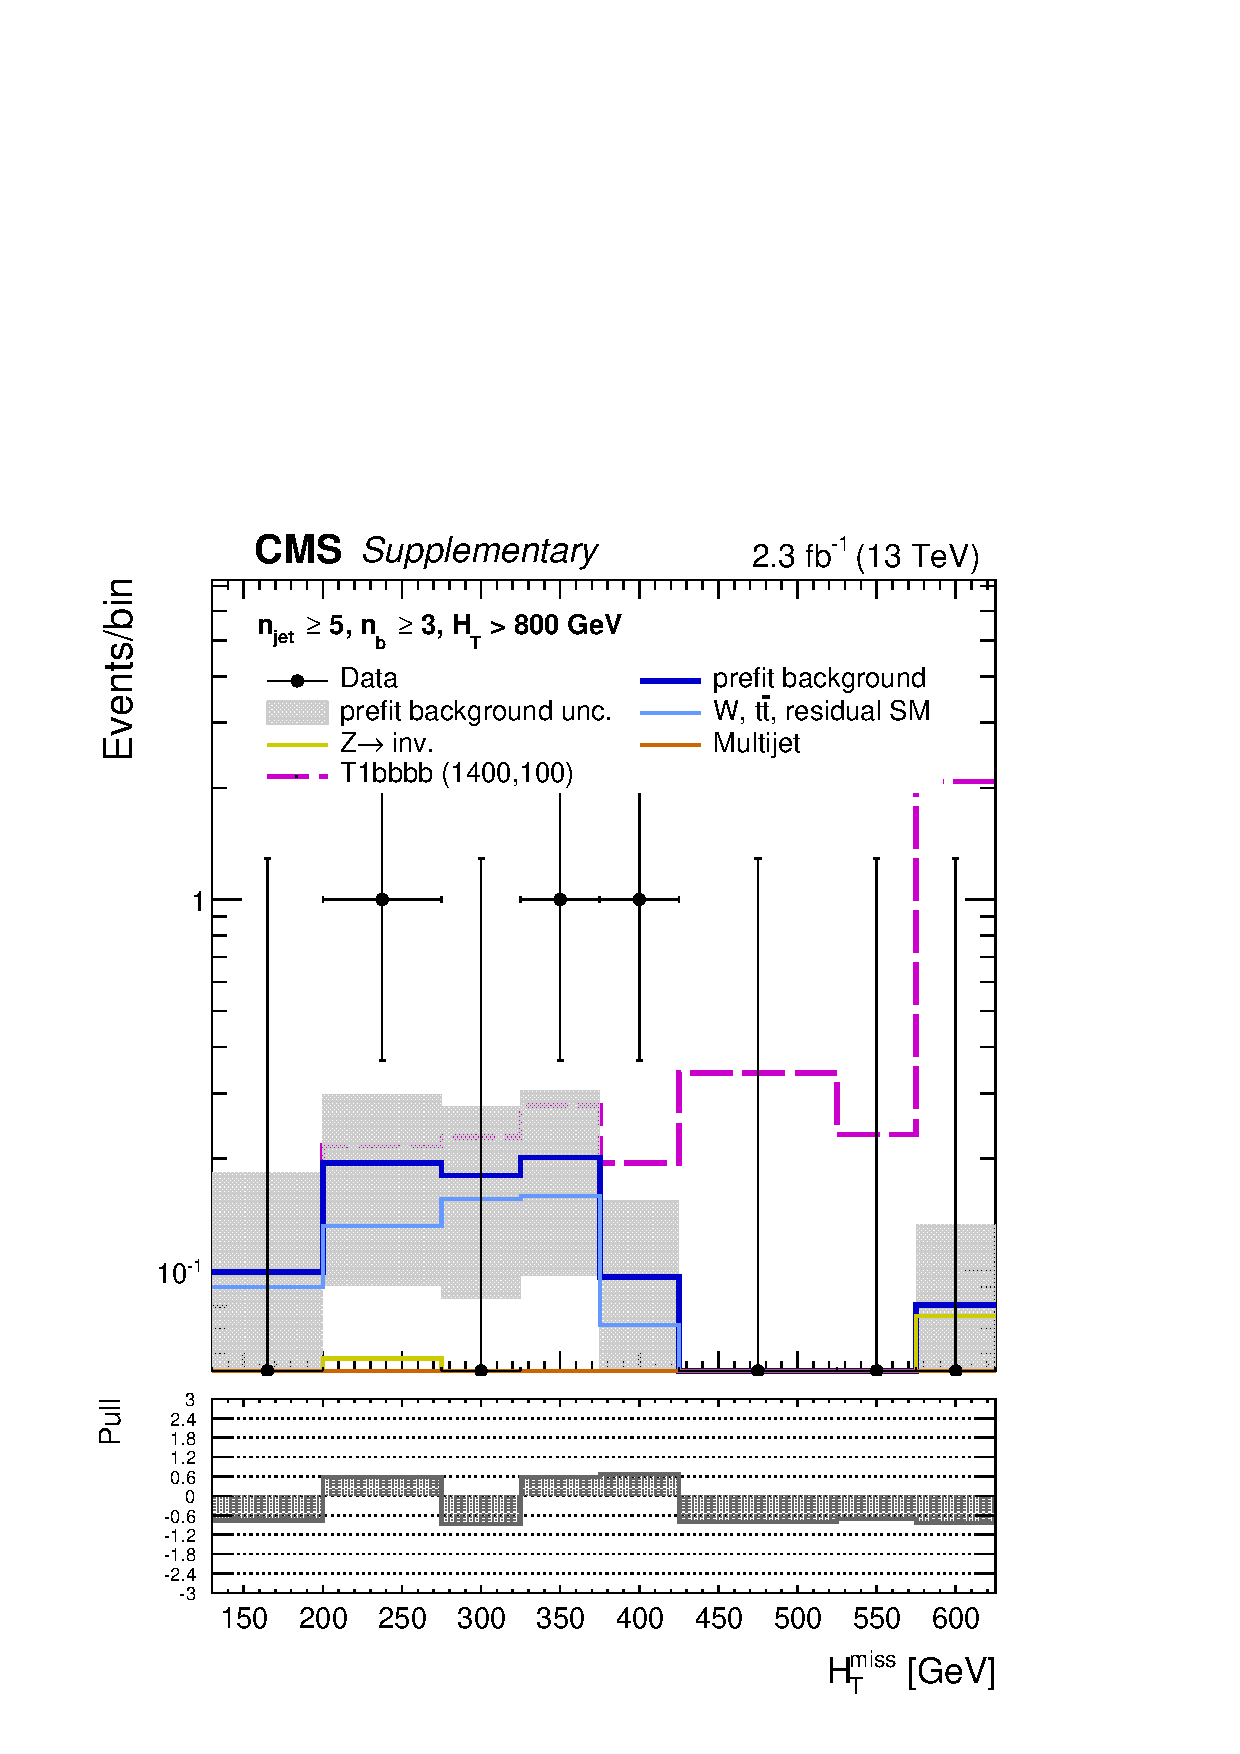
\includegraphics[width=0.45\textwidth]{figures/postFitShape_ge3b_ge5j_800_Inf_prefit_T1bbbb_1400_100} } ~~
    %% \subfigure[$\njet \geq 5$, $\nb = 0$, $600 < \scalht < 800$ GeV]{ 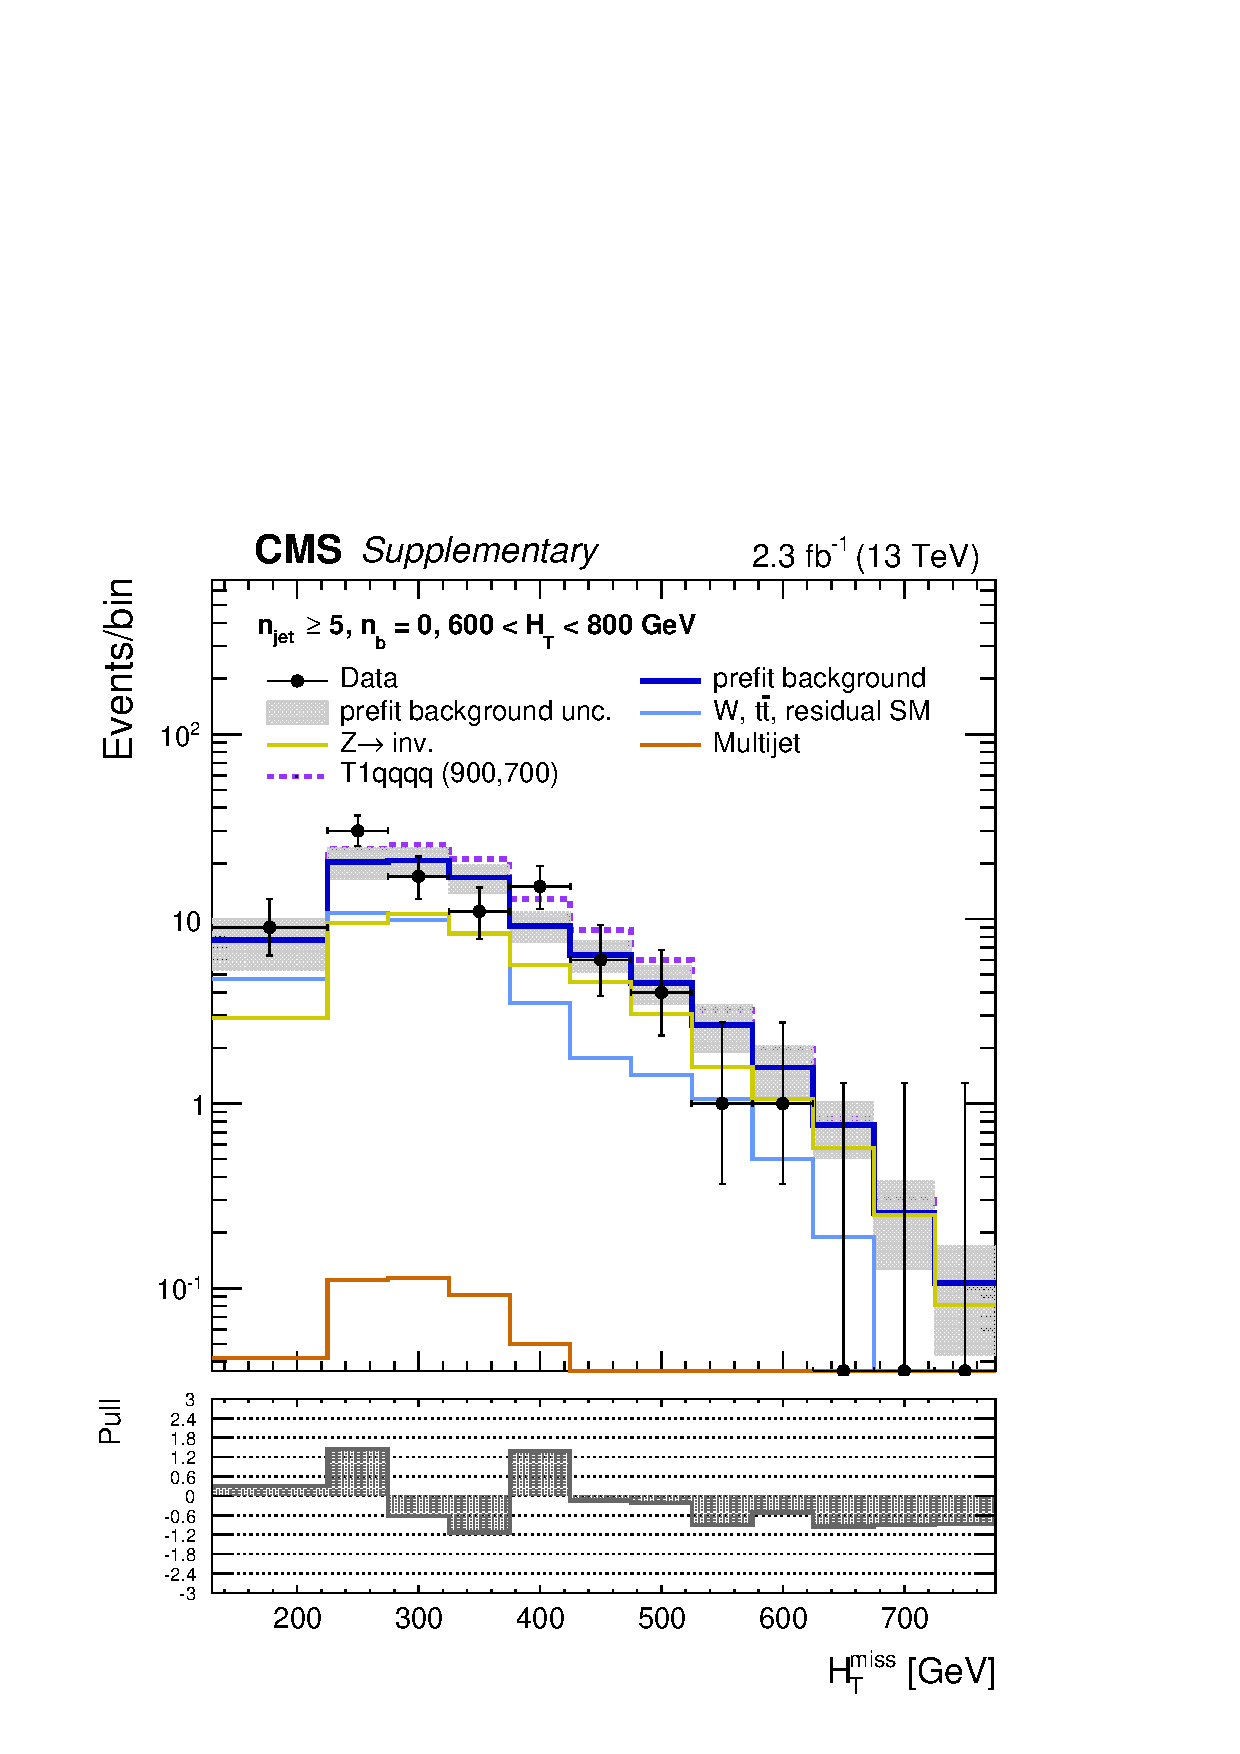
\includegraphics[width=0.45\textwidth]{figures/postFitShape_eq0b_ge5j_600_800_prefit_T1qqqq_900_700} } \\
    %% \subfigure[$\njet \geq 5$, $\nb = 1$, $\scalht > 800$ GeV]   { 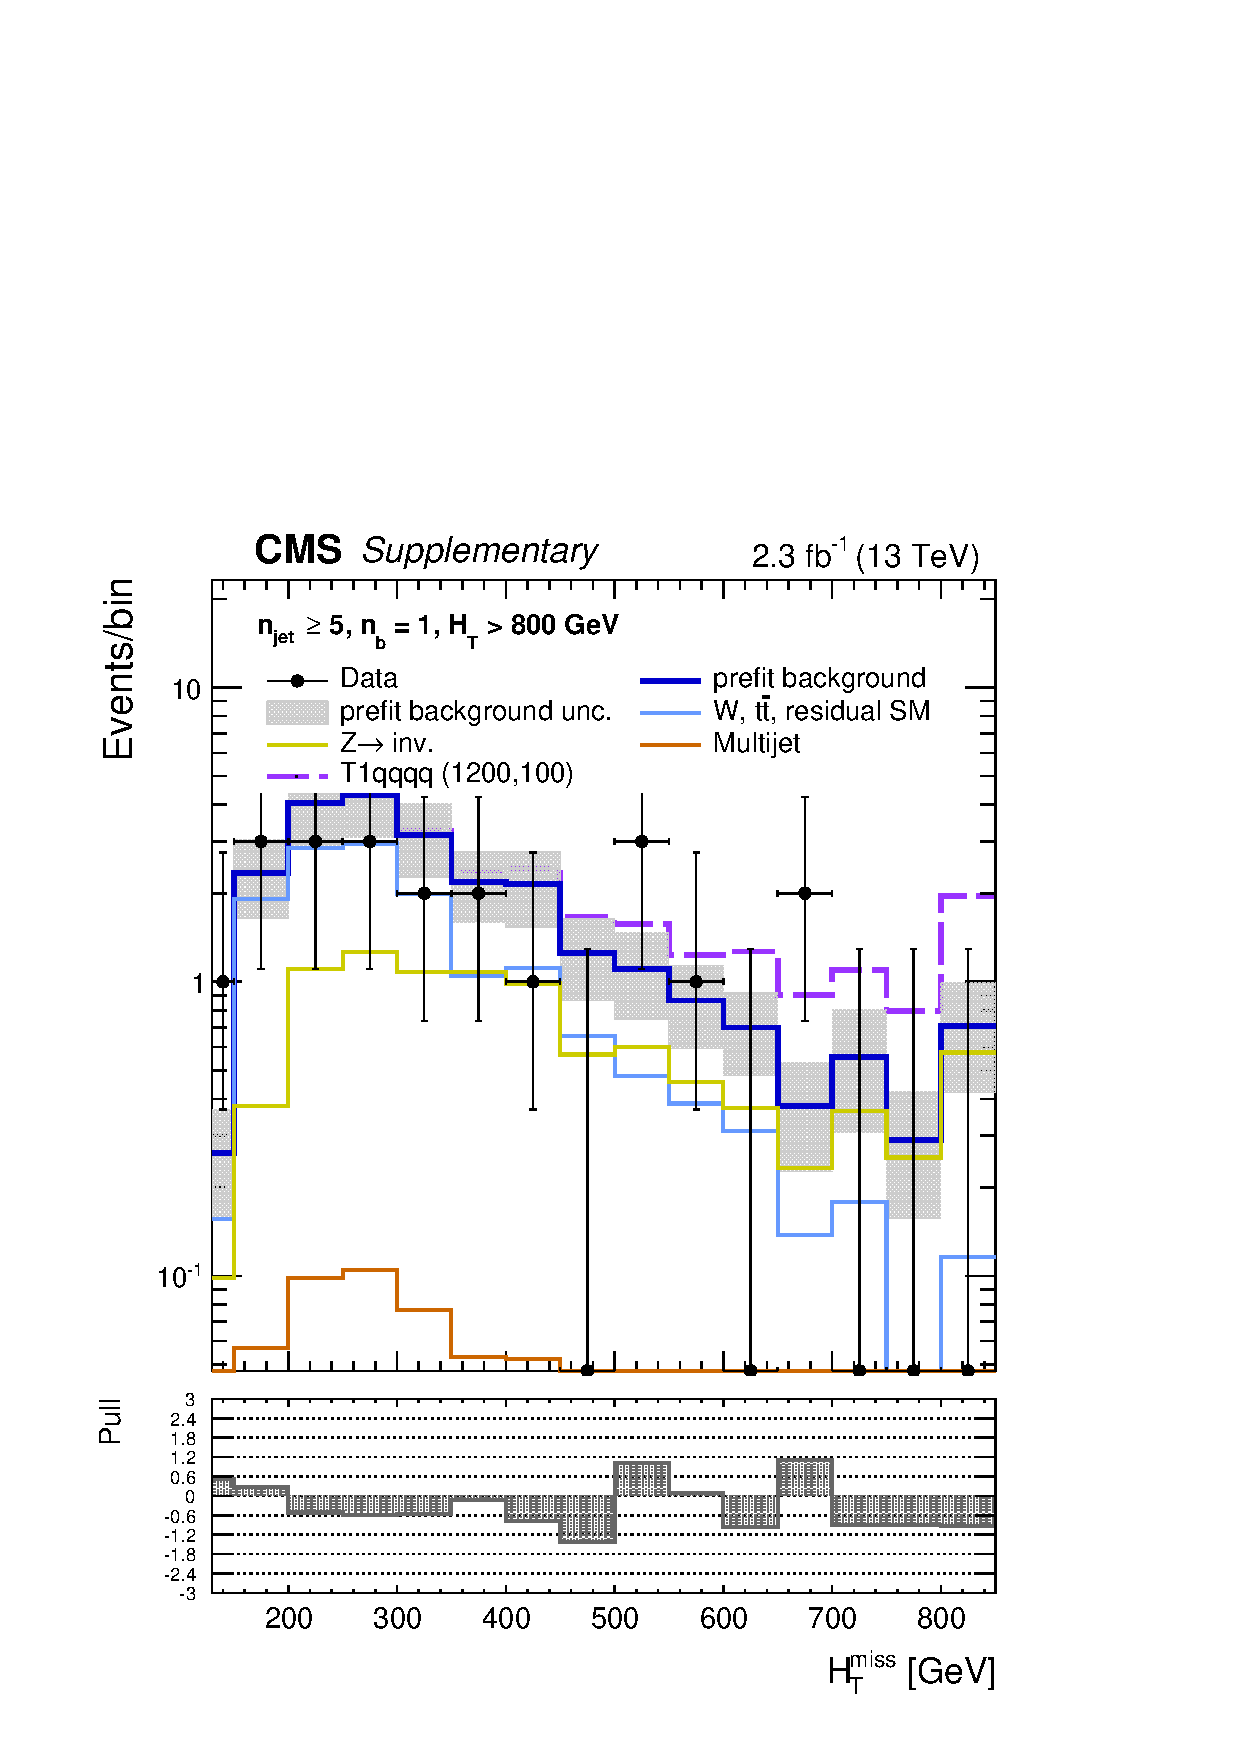
\includegraphics[width=0.45\textwidth]{figures/postFitShape_eq1b_ge5j_800_Inf_prefit_T1qqqq_1200_100} } ~~
    \subfigure[$\njet \geq 5$, $\nb = 2$, $\scalht > 800$ GeV]{ 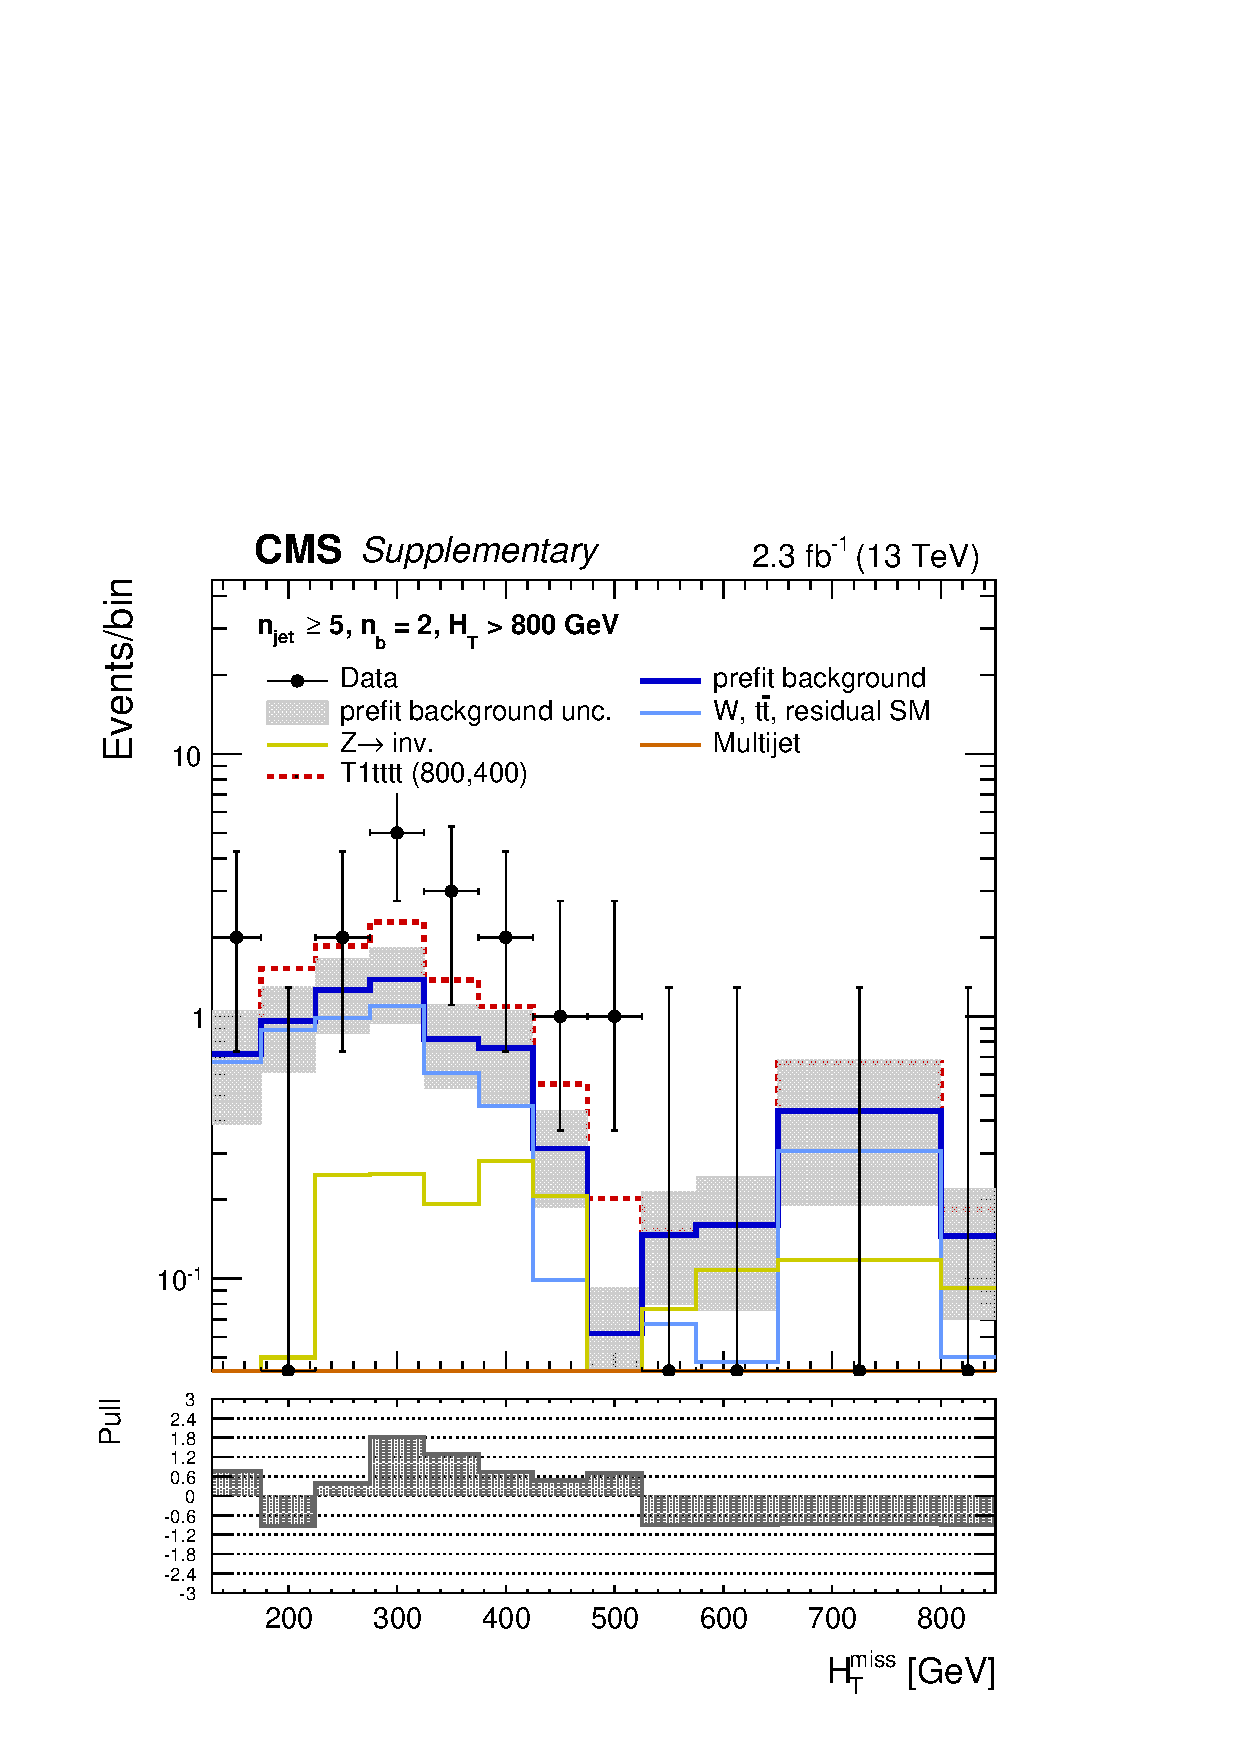
\includegraphics[width=0.45\textwidth]{figures/postFitShape_eq2b_ge5j_800_Inf_prefit_T1tttt_800_400} } \\
  \end{center}
\end{figure}



%% \clearpage
%% \begin{table}[h!]
%%   \caption{Representative range of uncertainty across the analysis bins 
%%     for each source of systematic uncertainty on the signal acceptance.
%%     Two benchmark points are chosen for each model, 
%%     corresponding to ``compressed'' and ``uncompressed'' scenarios, 
%%     i.e. with small and large mass splitting between the mother particle and the LSP.
%%     \label{tab:sig-systematics}   
%%   }
%%   \centering
%%   \begin{tabular}{ ccccccccc }
%%     \hline
%%     \hline
%% Model & ($m_{\mathrm{Susy}},m_{\mathrm{LSP}}$) & Luminosity & ISR & JEC & PU & b-tag & Trigger & MC stat. \\ \hline
%% \multirow{2}{*}{T1bbbb}
%%  & (1500,100) & 4.6\% & 1-2\% & 1-12\% & 1-4\% & 2-22\% & 1-3\% & 5-17\% \\ 
%%  & (1000,800) & 4.6\% & 1-17\% & 1-40\% & 1-20\% & 1-14\% & 1-15\% & 8-31\% \\ \hline 
%% \multirow{2}{*}{T1tttt}
%%  & (1300,100) & 4.6\% & 1-2\% & 2-7\% & 1-4\% & 2-12\% & 1-3\% & 7-16\% \\ 
%%  & (800,400) & 4.6\% & 1-2\% & 3-45\% & 1-13\% & 1-8\% & 1-10\% & 7-27\% \\ \hline 
%% \multirow{2}{*}{T1ttbb}
%%  & (1300,100) & 4.6\% & 1-2\% & 3-16\% & 1-18\% & 2-19\% & 1-4\% & 9-32\% \\ 
%%  & (1000,700) & 4.6\% & 1-9\% & 3-65\% & 1-12\% & 1-14\% & 1-14\% & 9-30\% \\ \hline 
%% \multirow{2}{*}{T5ttcc}
%%  & (1200,200) & 4.6\% & 5-25\% & 3-21\% & 1-9\% & 1-24\% & 2-6\% & 6-25\% \\ 
%%  & (750,600) & 4.6\% & 1-4\% & 5-21\% & 1-8\% & 1-3\% & 4-7\% & 9-23\% \\ \hline 
%% \multirow{2}{*}{T5ttttDM175}
%%  & (800,100) & 4.6\% & 2-4\% & 3-5\% & 2-6\% & 1-6\% & 3-6\% & 12-20\% \\ 
%%  & (700,400) & 4.6\% & 2-10\% & 10-10\% & 4-4\% & 2-2\% & 3-10\% & 20-20\% \\ \hline 
%% \multirow{2}{*}{T5tttt\_degen}
%%  & (1100,100) & 4.6\% & 12-16\% & 6-11\% & 3-5\% & 4-15\% & 3-4\% & 15-21\% \\ 
%%  & (800,600) & 4.6\% & 1-8\% & 1-34\% & 1-20\% & 1-7\% & 1-11\% & 5-32\% \\ \hline 
%% \multirow{2}{*}{T2tt}
%%  & (700,50) & 4.6\% & 1-4\% & 2-22\% & 1-13\% & 1-21\% & 2-11\% & 8-33\% \\ 
%%  & (350,100) & 4.6\% & 1-1\% & 1-28\% & 1-10\% & 1-7\% & 5-9\% & 7-31\% \\ \hline 
%% \multirow{1}{*}{T2cc}
%%  & (325,305) & 4.6\% & 1-27\% & 1-27\% & 1-26\% & 1-12\% & 5-16\% & 3-32\% \\ \hline 
%% \multirow{1}{*}{T2-4bd}
%%  & (300,290) & 4.6\% & 1-27\% & 1-25\% & 1-11\% & 1-12\% & 2-18\% & 2-27\% \\ \hline 
%% \multirow{1}{*}{T2mixed}
%%  & (300,250) & 4.6\% & 1-27\% & 1-33\% & 1-22\% & 1-13\% & 2-16\% & 3-33\% \\ \hline 
%% \multirow{2}{*}{T2tb}
%%  & (600,50) & 4.6\% & 1-3\% & 1-22\% & 1-8\% & 1-17\% & 1-12\% & 3-28\% \\ 
%%  & (350,225) & 4.6\% & 1-4\% & 2-41\% & 1-12\% & 1-8\% & 5-7\% & 9-33\% \\ \hline 
%% \multirow{2}{*}{T2bW\_X05}
%%  & (400,100) & 4.6\% & 1-2\% & 4-60\% & 1-9\% & 1-9\% & 5-9\% & 10-33\% \\ 
%%  & (300,175) & 4.6\% & 2-2\% & 1-24\% & 1-11\% & 1-6\% & 9-9\% & 9-33\% \\ \hline 
%% \multirow{2}{*}{T2bb}
%%  & (800,50) & 4.6\% & 2-6\% & 1-21\% & 1-16\% & 1-23\% & 2-12\% & 5-31\% \\ 
%%  & (375,300) & 4.6\% & 1-10\% & 3-25\% & 1-11\% & 1-7\% & 3-3\% & 8-33\% \\ \hline 
%% \multirow{2}{*}{T1qqqq}
%%  & (1300,100) & 4.6\% & 2-2\% & 4-21\% & 1-5\% & 2-14\% & 1-3\% & 7-30\% \\ 
%%  & (900,700) & 4.6\% & 1-13\% & 1-26\% & 1-9\% & 1-10\% & 5-13\% & 10-33\% \\ \hline 
%% \multirow{2}{*}{T2qq}
%%  & (1050,100) & 4.6\% & 2-5\% & 3-16\% & 1-10\% & 1-11\% & 1-6\% & 7-33\% \\ 
%%  & (650,550) & 4.6\% & 3-9\% & 2-28\% & 1-15\% & 1-6\% & 3-12\% & 10-28\% \\ \hline 
%%     \hline
%%   \end{tabular}
%% \end{table}


\clearpage
\begin{table}[h!] 
  \scriptsize
  \caption{ 
  Signal yield, background expectation and data observation for the 10 most excluding (\nj,\nb,\scalht) category for T1bbbb benchamark models. 
  Expected and observed upper limits on the signal strength $r=\sigma/\sigma_{\mathrm{theo}}$ are also shown 
  for each individual bin and for the 4 most excluding \nj categories combined (with all the \nb,\scalht bin with each category).
  It should be kept in mind that in the analysis jet categories are always considered with all their \nb,\scalht bins 
  combined, in order to preserve the correlation of the systematic uncertainties. 
  Therefore the individual-bin limits shown in this table have to be regarded only as an approximate indication 
  of the sensitivity of each bin, as some of the correlations may be neglected.
  \label{tab:sigBenchmarksYields_T1bbbb}}
  \centering 
  \begin{tabular}{ lllllll } 
    \hline 
    \hline 
    Model & Analysis bin & Signal & Background & Data & Exp. U. L. & Obs. U. L. \\ \hline
\multirow{10}{*}{\parbox[t]{2cm}{T1bbbb (1500,100)\\exp.: $r<0.81$\\obs.: $r<0.79$}}
 & $\nj \geq5j,\nb \geq3$, $\scalht > 800 \, \mathrm{GeV}$ & 1.6 & $0.9 \pm 0.3 \mathrm{(syst.)} ^{+2.3}_{-1.9} \mathrm{(stat.)}$ & 3 & $r < 1.5$ & $r < 1.7$\\ 
 & $\nj \geq5j,\nb =2$, $\scalht > 800 \, \mathrm{GeV}$ & 1.8 & $7.2 \pm 2.2 \mathrm{(syst.)} ^{+4.8}_{-3.7} \mathrm{(stat.)}$ & 16 & $r < 2.0$ & $r < 2.3$\\ 
 & $\nj \geq5j,\nb =1$, $\scalht > 800 \, \mathrm{GeV}$ & 1.2 & $24.3 \pm 6.4 \mathrm{(syst.)} ^{+5.3}_{-4.7} \mathrm{(stat.)}$ & 21 & $r < 4.8$ & $r < 4.9$\\ 
 & $\nj =4j,\nb \geq3$, $\scalht > 800 \, \mathrm{GeV}$ & 0.5 & $0.1 \pm 0.0 \mathrm{(syst.)} ^{+1.3}_{-0.0} \mathrm{(stat.)}$ & 0 & $r < 5.0$ & $r < 4.5$\\ 
 & $\nj =4j,\nb =2$, $\scalht > 800 \, \mathrm{GeV}$ & 0.7 & $3.4 \pm 1.1 \mathrm{(syst.)} ^{+2.3}_{-1.3} \mathrm{(stat.)}$ & 2 & $r < 5.4$ & $r < 4.5$\\ 
 & $\nj =4j,\nb =1$, $\scalht > 800 \, \mathrm{GeV}$ & 0.5 & $14.4 \pm 3.6 \mathrm{(syst.)} ^{+3.8}_{-3.2} \mathrm{(stat.)}$ & 10 & $r < 12.9$ & $r < 10.3$\\ 
 & $\nj =3j,\nb =2$, $\scalht > 800 \, \mathrm{GeV}$ & 0.1 & $1.3 \pm 0.4 \mathrm{(syst.)} ^{+1.8}_{-0.6} \mathrm{(stat.)}$ & 1 & $r < 22.1$ & $r < 26.5$\\ 
 & $\nj =3j,\nb =1$, $\scalht > 800 \, \mathrm{GeV}$ & 0.2 & $11.6 \pm 3.1 \mathrm{(syst.)} ^{+3.8}_{-3.2} \mathrm{(stat.)}$ & 10 & $r < 32.1$ & $r < 27.1$\\ 
 & $\nj \geq5j,\nb =0$, $\scalht > 800 \, \mathrm{GeV}$ & 0.3 & $63.1 \pm 15.1 \mathrm{(syst.)} ^{+8.0}_{-8.0} \mathrm{(stat.)}$ & 64 & $r < 48.6$ & $r < 45.8$\\ 
 & $\nj =3j,\nb \geq3$, $\scalht > 400 \, \mathrm{GeV}$ & 0.0 & $0.5 \pm 0.2 \mathrm{(syst.)} ^{+1.8}_{-0.6} \mathrm{(stat.)}$ & 1 & $r < 64.6$ & $r < 82.4$\\ \hline
\multirow{10}{*}{\parbox[t]{2cm}{T1bbbb (1000,800)\\exp.: $r<0.33$\\obs.: $r<0.32$}}
 & $\nj \geq5j,\nb \geq3$, $\scalht > 800 \, \mathrm{GeV}$ & 3.6 & $0.9 \pm 0.3 \mathrm{(syst.)} ^{+2.3}_{-1.9} \mathrm{(stat.)}$ & 3 & $r < 0.9$ & $r < 1.6$\\ 
 & $\nj \geq5j,\nb =2$, $\scalht > 800 \, \mathrm{GeV}$ & 4.6 & $7.2 \pm 2.2 \mathrm{(syst.)} ^{+4.8}_{-3.7} \mathrm{(stat.)}$ & 16 & $r < 1.1$ & $r < 2.9$\\ 
 & $\nj \geq5j,\nb \geq3$, $600 < \scalht < 800 \mathrm{GeV}$ & 2.9 & $1.5 \pm 0.4 \mathrm{(syst.)} ^{+1.8}_{-0.6} \mathrm{(stat.)}$ & 1 & $r < 1.2$ & $r < 0.9$\\ 
 & $\nj \geq5j,\nb =2$, $600 < \scalht < 800 \mathrm{GeV}$ & 3.9 & $10.9 \pm 2.9 \mathrm{(syst.)} ^{+3.8}_{-3.2} \mathrm{(stat.)}$ & 10 & $r < 1.8$ & $r < 1.5$\\ 
 & $\nj \geq5j,\nb \geq3$, $500 < \scalht < 600 \mathrm{GeV}$ & 2.2 & $3.0 \pm 1.1 \mathrm{(syst.)} ^{+1.8}_{-0.6} \mathrm{(stat.)}$ & 1 & $r < 2.2$ & $r < 1.4$\\ 
 & $\nj \geq5j,\nb \geq3$, $400 < \scalht < 500 \mathrm{GeV}$ & 1.6 & $1.4 \pm 0.4 \mathrm{(syst.)} ^{+1.8}_{-0.6} \mathrm{(stat.)}$ & 1 & $r < 2.4$ & $r < 2.1$\\ 
 & $\nj =4j,\nb \geq3$, $400 < \scalht < 500 \mathrm{GeV}$ & 1.9 & $2.8 \pm 0.9 \mathrm{(syst.)} ^{+1.3}_{-0.0} \mathrm{(stat.)}$ & 0 & $r < 2.5$ & $r < 1.4$\\ 
 & $\nj \geq5j,\nb =1$, $\scalht > 800 \, \mathrm{GeV}$ & 3.2 & $24.3 \pm 6.4 \mathrm{(syst.)} ^{+5.3}_{-4.7} \mathrm{(stat.)}$ & 21 & $r < 2.9$ & $r < 2.8$\\ 
 & $\nj =3a,\nb \geq3$, $\scalht > 300 \, \mathrm{GeV}$ & 1.0 & $0.7 \pm 0.2 \mathrm{(syst.)} ^{+1.8}_{-0.6} \mathrm{(stat.)}$ & 1 & $r < 3.4$ & $r < 3.8$\\ 
 & $\nj \geq5a,\nb \geq3$, $400 < \scalht < 500 \mathrm{GeV}$ & 1.5 & $4.5 \pm 1.2 \mathrm{(syst.)} ^{+2.8}_{-2.2} \mathrm{(stat.)}$ & 5 & $r < 3.6$ & $r < 4.3$\\ \hline
    \hline
  \end{tabular}
\end{table}


\clearpage
\begin{table}[h!] 
  \scriptsize
  \caption{ 
  Signal yield, background expectation and data observation for the 10 most excluding (\nj,\nb,\scalht) category for T1tttt benchamark models. 
  Expected and observed upper limits on the signal strength $r=\sigma/\sigma_{\mathrm{theo}}$ are also shown 
  for each individual bin and for the 4 most excluding \nj categories combined (with all the \nb,\scalht bin with each category).
  It should be kept in mind that in the analysis jet categories are always considered with all their \nb,\scalht bins 
  combined, in order to preserve the correlation of the systematic uncertainties. 
  Therefore the individual-bin limits shown in this table have to be regarded only as an approximate indication 
  of the sensitivity of each bin, as some of the correlations may be neglected.
  \label{tab:sigBenchmarksYields_T1tttt}}
  \centering 
  \begin{tabular}{ lllllll } 
    \hline 
    \hline 
    Model & Analysis bin & Signal & Background & Data & Exp. U. L. & Obs. U. L. \\ \hline
\multirow{10}{*}{\parbox[t]{2cm}{T1tttt (1300,100)\\exp.: $r<1.0$\\obs.: $r<1.89$}}
 & $\nj \geq5j,\nb \geq3$, $\scalht > 800 \, \mathrm{GeV}$ & 1.8 & $0.9 \pm 0.3 \mathrm{(syst.)} ^{+2.3}_{-1.9} \mathrm{(stat.)}$ & 3 & $r < 1.5$ & $r < 2.1$\\ 
 & $\nj \geq5j,\nb =2$, $\scalht > 800 \, \mathrm{GeV}$ & 1.9 & $7.2 \pm 2.2 \mathrm{(syst.)} ^{+4.8}_{-3.7} \mathrm{(stat.)}$ & 16 & $r < 2.2$ & $r < 3.4$\\ 
 & $\nj \geq5j,\nb =1$, $\scalht > 800 \, \mathrm{GeV}$ & 1.2 & $24.3 \pm 6.4 \mathrm{(syst.)} ^{+5.3}_{-4.7} \mathrm{(stat.)}$ & 21 & $r < 6.3$ & $r < 7.1$\\ 
 & $\nj \geq5j,\nb =0$, $\scalht > 800 \, \mathrm{GeV}$ & 0.3 & $63.1 \pm 15.1 \mathrm{(syst.)} ^{+8.0}_{-8.0} \mathrm{(stat.)}$ & 64 & $r < 48.8$ & $r < 57.2$\\ 
 & $\nj \geq5j,\nb \geq3$, $600 < \scalht < 800 \mathrm{GeV}$ & 0.0 & $1.5 \pm 0.4 \mathrm{(syst.)} ^{+1.8}_{-0.6} \mathrm{(stat.)}$ & 1 & $r < 148.8$ & $r < 108.3$\\ 
 & $\nj \geq5j,\nb =2$, $600 < \scalht < 800 \mathrm{GeV}$ & 0.0 & $10.9 \pm 2.9 \mathrm{(syst.)} ^{+3.8}_{-3.2} \mathrm{(stat.)}$ & 10 & $r < 151.6$ & $r < 95.3$\\ 
 & $\nj \geq5j,\nb =1$, $600 < \scalht < 800 \mathrm{GeV}$ & 0.0 & $38.0 \pm 8.3 \mathrm{(syst.)} ^{+5.9}_{-5.9} \mathrm{(stat.)}$ & 35 & $r < 165.8$ & $r < 145.4$\\ 
 & $\nj \geq5a,\nb =1$, $\scalht > 600 \, \mathrm{GeV}$ & 0.0 & $1.9 \pm 0.9 \mathrm{(syst.)} ^{+1.3}_{-0.0} \mathrm{(stat.)}$ & 0 & $r < 199.5$ & $r < 128.6$\\ 
 & $\nj =4j,\nb =1$, $\scalht > 800 \, \mathrm{GeV}$ & 0.0 & $14.4 \pm 3.6 \mathrm{(syst.)} ^{+3.8}_{-3.2} \mathrm{(stat.)}$ & 10 & $r < 261.6$ & $r < 196.4$\\ 
 & $\nj =4j,\nb =2$, $\scalht > 800 \, \mathrm{GeV}$ & 0.0 & $3.4 \pm 1.1 \mathrm{(syst.)} ^{+2.3}_{-1.3} \mathrm{(stat.)}$ & 2 & $r < 319.2$ & $r < 392.0$\\ \hline
\multirow{10}{*}{\parbox[t]{2cm}{T1tttt (800,400)\\exp.: $r<0.56$\\obs.: $r<1.03$}}
 & $\nj \geq5j,\nb \geq3$, $\scalht > 800 \, \mathrm{GeV}$ & 2.8 & $0.9 \pm 0.3 \mathrm{(syst.)} ^{+2.3}_{-1.9} \mathrm{(stat.)}$ & 3 & $r < 1.2$ & $r < 2.6$\\ 
 & $\nj \geq5j,\nb =2$, $\scalht > 800 \, \mathrm{GeV}$ & 3.8 & $7.2 \pm 2.2 \mathrm{(syst.)} ^{+4.8}_{-3.7} \mathrm{(stat.)}$ & 16 & $r < 1.9$ & $r < 5.1$\\ 
 & $\nj \geq5a,\nb \geq3$, $\scalht > 500 \, \mathrm{GeV}$ & 1.6 & $0.8 \pm 0.3 \mathrm{(syst.)} ^{+1.8}_{-0.6} \mathrm{(stat.)}$ & 1 & $r < 2.2$ & $r < 2.5$\\ 
 & $\nj \geq5j,\nb \geq3$, $600 < \scalht < 800 \mathrm{GeV}$ & 1.7 & $1.5 \pm 0.4 \mathrm{(syst.)} ^{+1.8}_{-0.6} \mathrm{(stat.)}$ & 1 & $r < 2.5$ & $r < 2.2$\\ 
 & $\nj \geq5a,\nb =2$, $\scalht > 600 \, \mathrm{GeV}$ & 1.0 & $0.5 \pm 0.3 \mathrm{(syst.)} ^{+1.8}_{-0.6} \mathrm{(stat.)}$ & 1 & $r < 2.9$ & $r < 3.4$\\ 
 & $\nj \geq5j,\nb =2$, $600 < \scalht < 800 \mathrm{GeV}$ & 2.7 & $10.9 \pm 2.9 \mathrm{(syst.)} ^{+3.8}_{-3.2} \mathrm{(stat.)}$ & 10 & $r < 3.2$ & $r < 4.3$\\ 
 & $\nj \geq5j,\nb =1$, $\scalht > 800 \, \mathrm{GeV}$ & 3.1 & $24.3 \pm 6.4 \mathrm{(syst.)} ^{+5.3}_{-4.7} \mathrm{(stat.)}$ & 21 & $r < 3.8$ & $r < 4.0$\\ 
 & $\nj \geq5a,\nb =2$, $500 < \scalht < 600 \mathrm{GeV}$ & 1.8 & $6.1 \pm 2.1 \mathrm{(syst.)} ^{+3.3}_{-2.2} \mathrm{(stat.)}$ & 6 & $r < 4.0$ & $r < 3.7$\\ 
 & $\nj \geq5a,\nb =2$, $400 < \scalht < 500 \mathrm{GeV}$ & 2.6 & $29.1 \pm 6.3 \mathrm{(syst.)} ^{+5.8}_{-5.2} \mathrm{(stat.)}$ & 29 & $r < 5.5$ & $r < 3.9$\\ 
 & $\nj \geq5j,\nb =1$, $600 < \scalht < 800 \mathrm{GeV}$ & 3.2 & $38.0 \pm 8.3 \mathrm{(syst.)} ^{+5.9}_{-5.9} \mathrm{(stat.)}$ & 35 & $r < 5.6$ & $r < 5.3$\\ \hline
    \hline
  \end{tabular}
\end{table}


\clearpage
\begin{figure*}[t]
  \begin{center}
    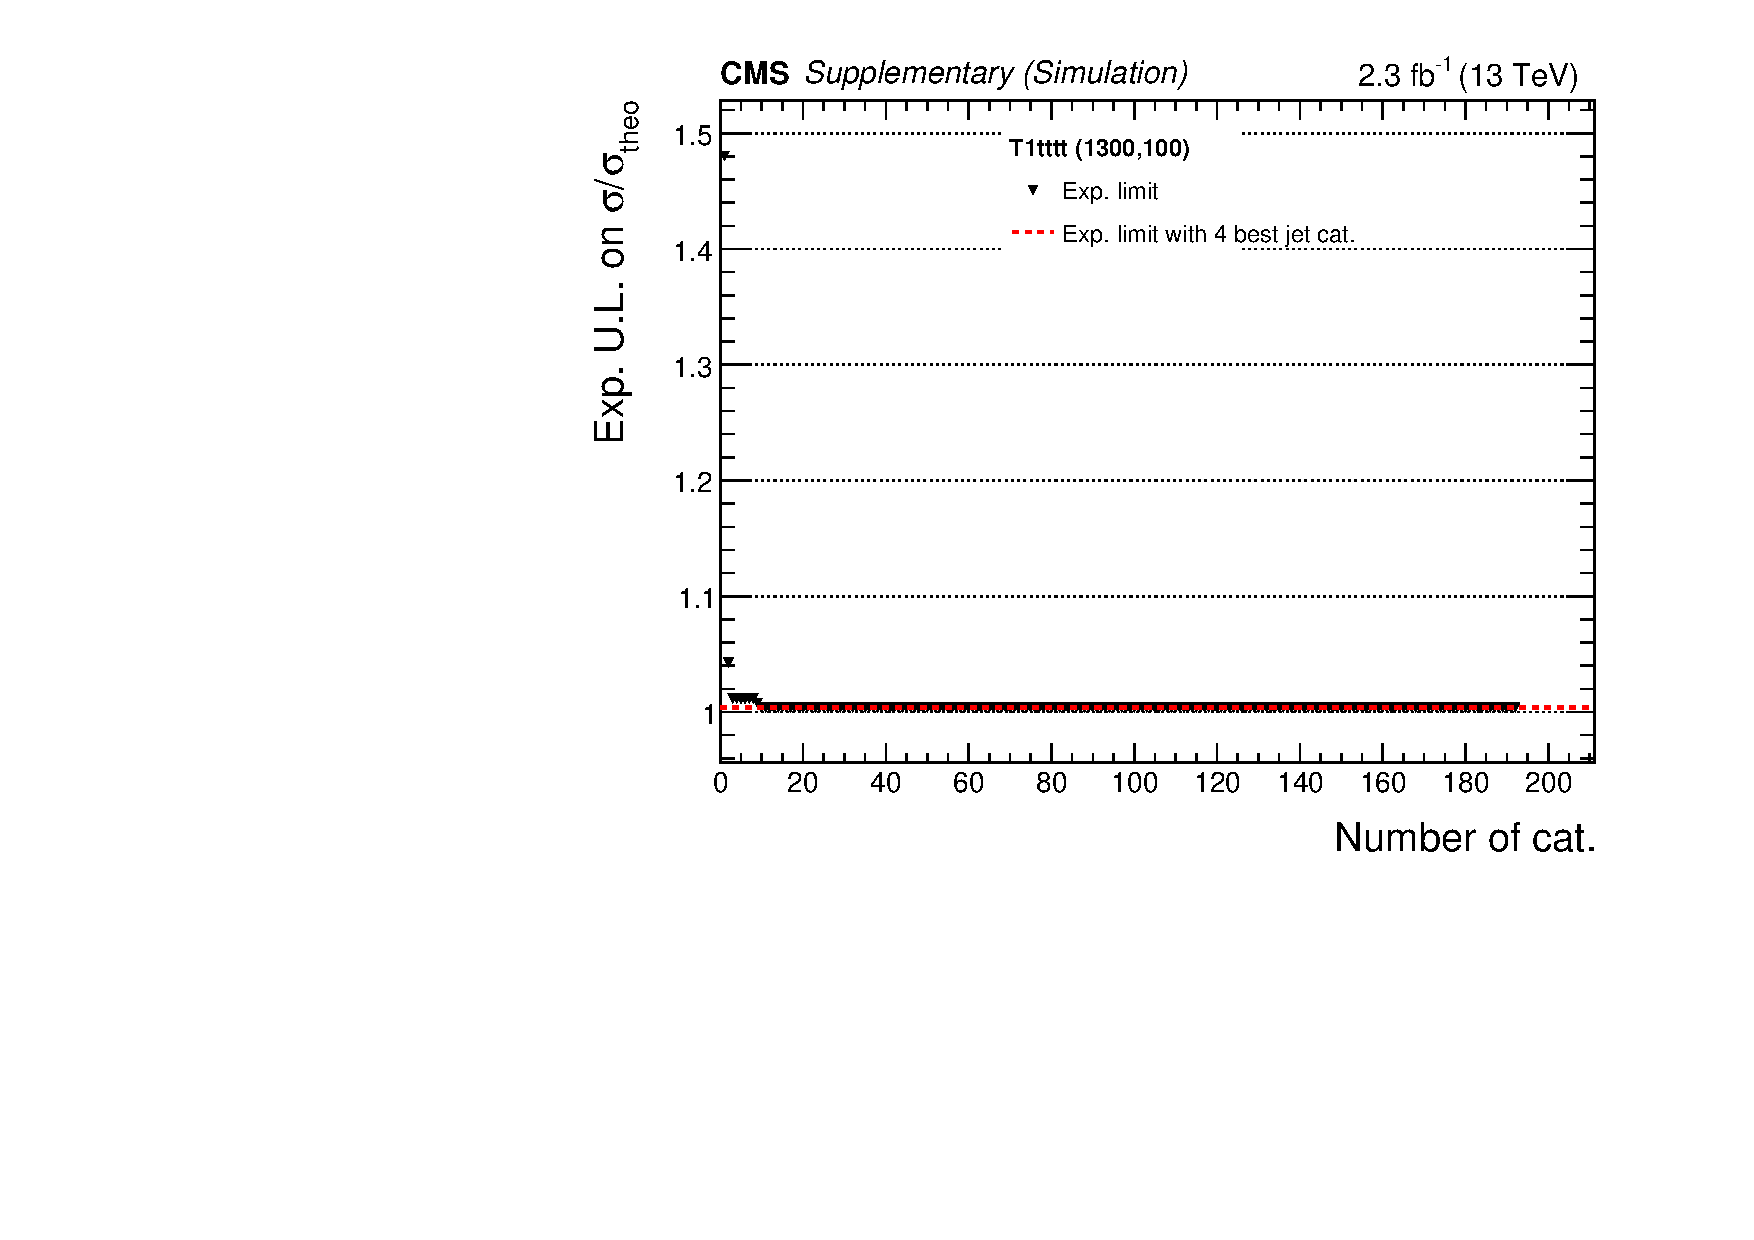
\includegraphics[width=0.49\textwidth]{supplementary/figures/expVsCat_SMS-T1tttt_mGluino-1300_mLSP-100_25ns} \, 
    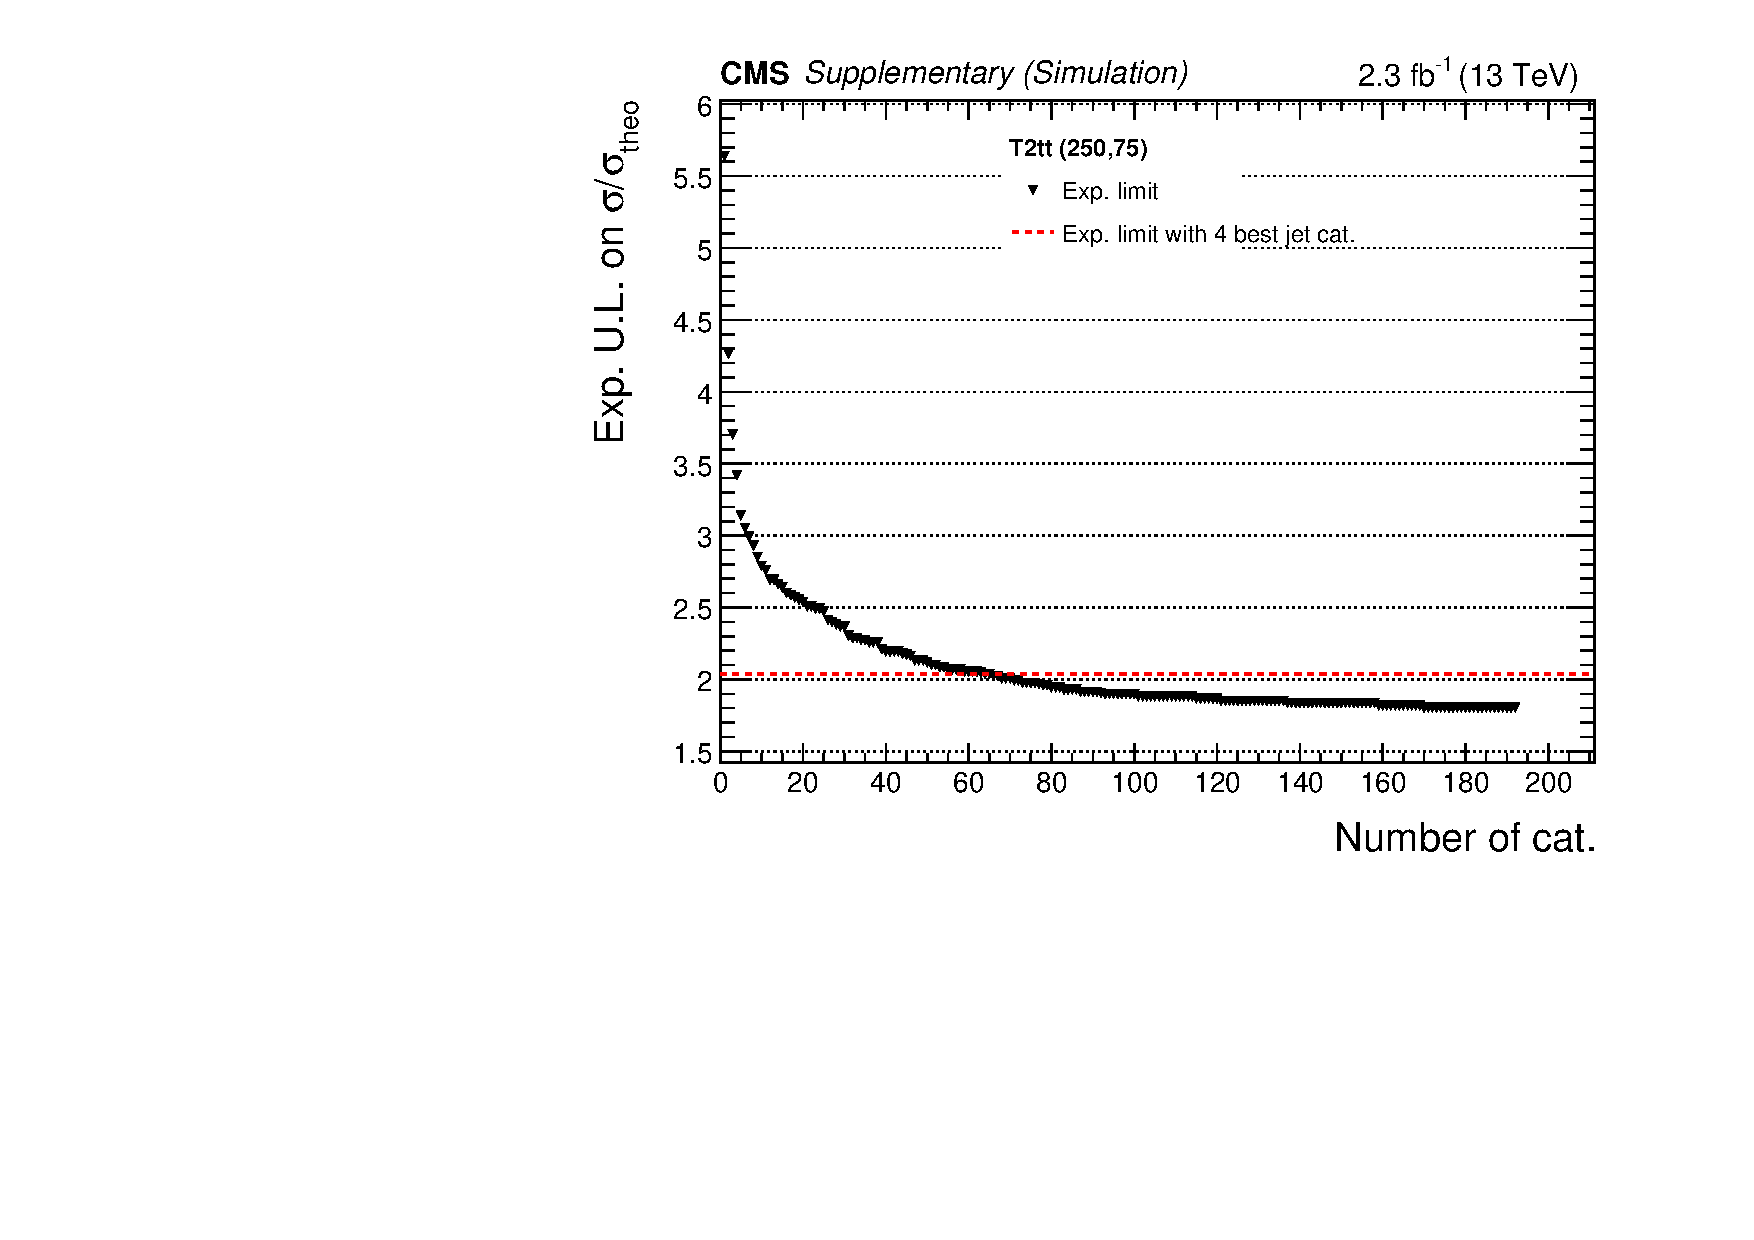
\includegraphics[width=0.49\textwidth]{supplementary/figures/expVsCat_SMS-T2tt_mStop-250_mLSP-75_25ns} \,     
  \end{center}
  \caption{
  The expected upper limit (black points) on the signal strength $\sigma/\sigma_{\mathrm{theo}}$ as a function of the number of 
  (\nj,\nb,\scalht) categories included in the fit, where the categories are ranked according to the expected exclusion, 
  for one T1tttt (T2tt) benchmark point on the left (right) plot. 
  The red dashed line is the expected upper limit using the most excluding 4 jet categories (with all the \nb,\scalht bins within each jet category), 
  as it used for the final limit calculation in this analysis. 
  For the purpose of this test the MC statistical uncertainty in each bin has not been considered. 
  It should be kept in mind that in the analysis jet categories are always considered with all their \nb,\scalht bins 
  combined, in order to preserve the correlation of the systematic uncertainties. 
  Therefore the study depicted by the black points has to be regarded only as an approximate indication 
  of the number of categories contributing to the exclusion, as some of the correlations may be neglected.
  \label{fig:sensitivityVsCat}}
\end{figure*}



\clearpage
\begin{figure*}[tb]
 \begin{center}
   \subfigure[\texttt{T1qqqq}]{
     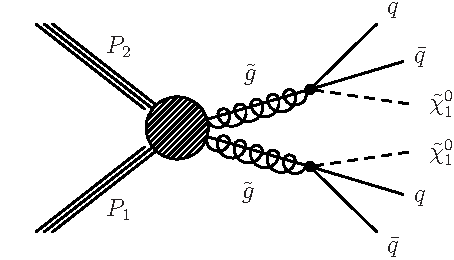
\includegraphics[height=0.15\textwidth]{figures/T1qqqq_feyn}
     \label{fig:T1qqqq_feyn}
   } ~~
   \subfigure[\texttt{T2qq}]{
     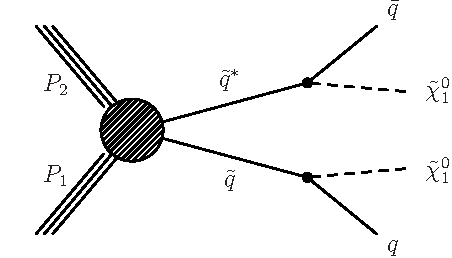
\includegraphics[height=0.15\textwidth]{figures/T2qq_feyn}
     \label{fig:T2qq_feyn}
   } \\
   \subfigure[\texttt{T1bbbb}]{
     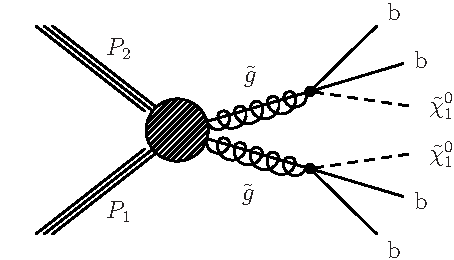
\includegraphics[height=0.15\textwidth]{figures/T1bbbb_feyn}
     \label{fig:T1bbbb_feyn}
   } ~~
   \subfigure[\texttt{T1tttt}]{
     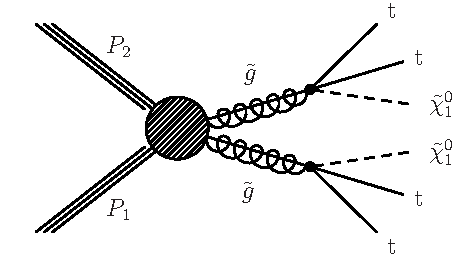
\includegraphics[height=0.15\textwidth]{figures/T1tttt_feyn}
     \label{fig:T1tttt_feyn}
   } ~~
   \subfigure[\texttt{T1ttbb}]{
     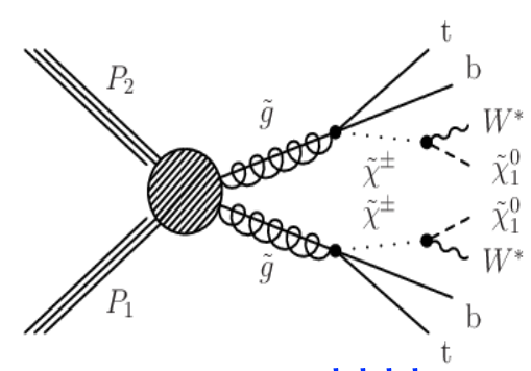
\includegraphics[height=0.15\textwidth]{figures/T1ttbb_feyn}
     \label{fig:T1ttbb_feyn}
   } \\
   \subfigure[\texttt{T5tttt}]{
     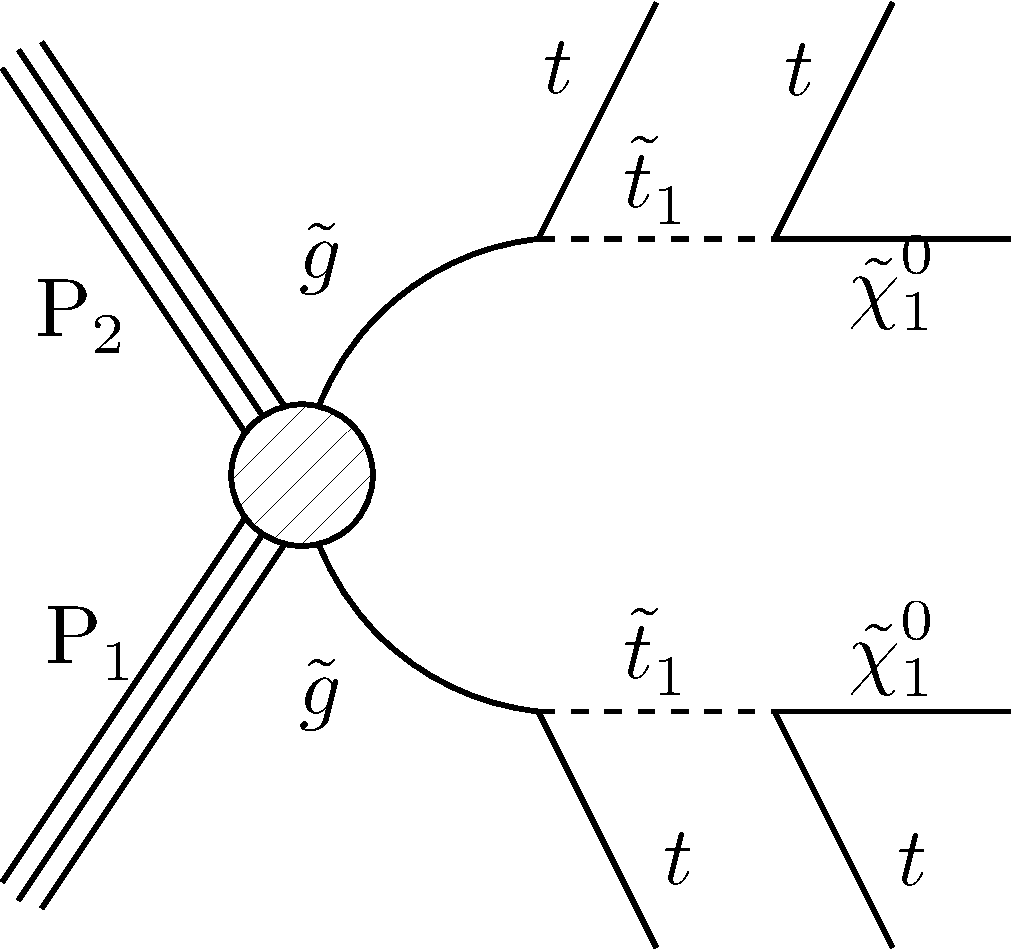
\includegraphics[height=0.15\textwidth]{figures/T5tttt_feyn}
     \label{fig:T5tttt_feyn}
   } ~~
   \subfigure[\texttt{T5ttcc}]{
     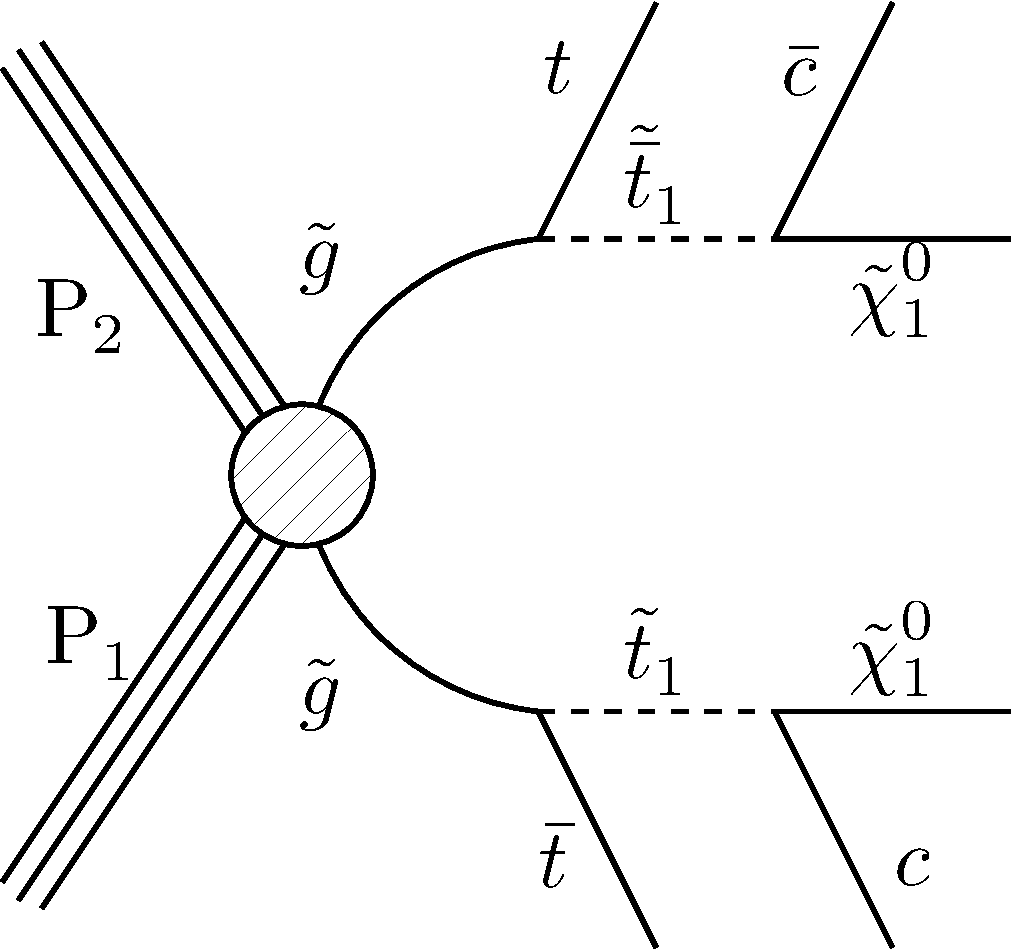
\includegraphics[height=0.15\textwidth]{figures/T5ttcc_feyn}
     \label{fig:T5ttcc_feyn}
   } ~~
   \subfigure[\texttt{T5tttt\_degen}]{
     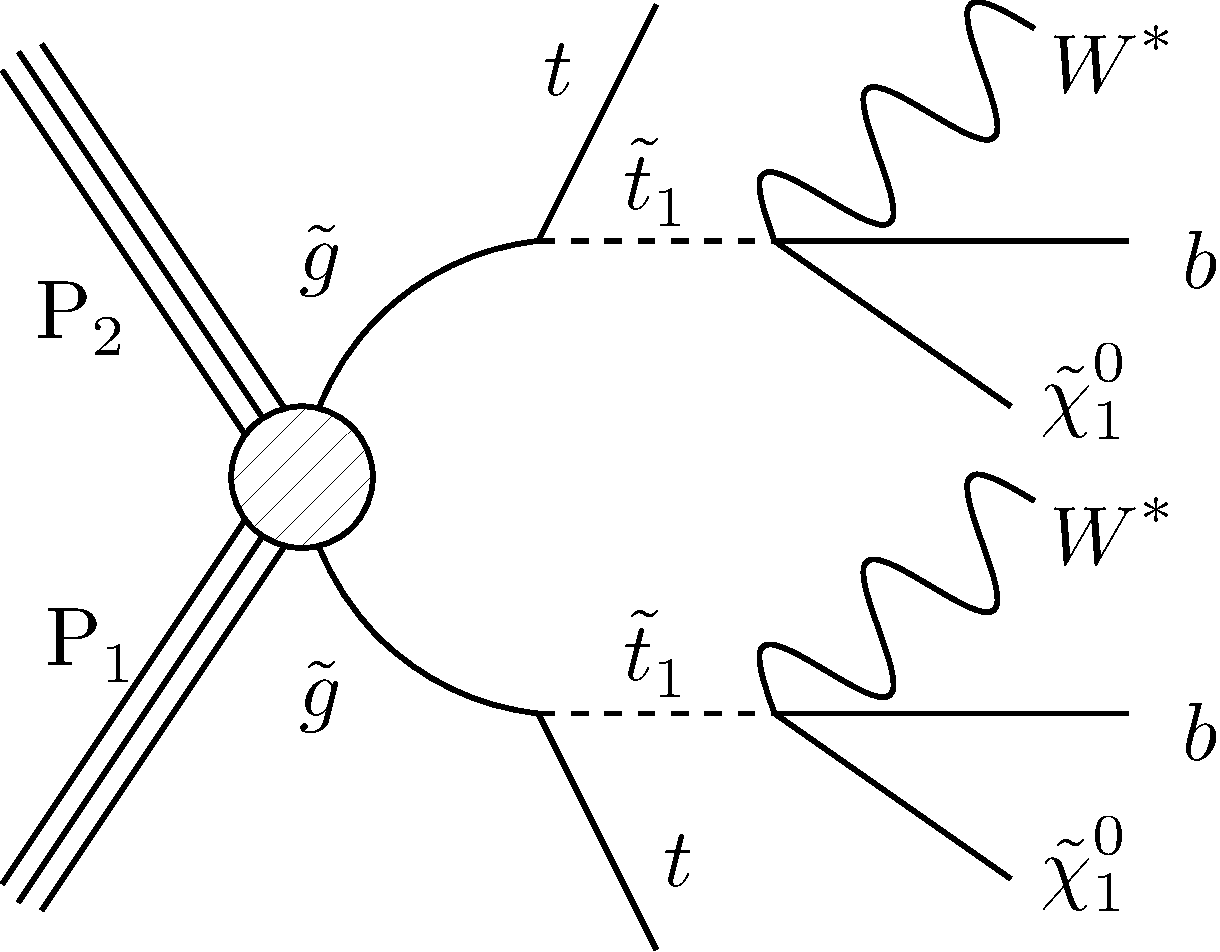
\includegraphics[height=0.15\textwidth]{figures/T5tttt_degen_feyn}
     \label{fig:T5tttt_degen_feyn}
   } \\
   \subfigure[\texttt{T2bb}]{
     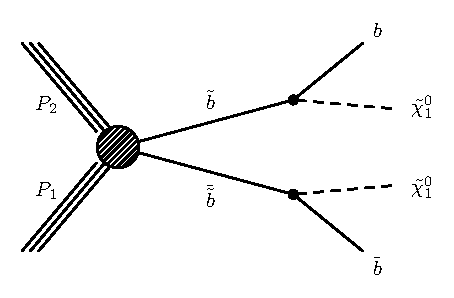
\includegraphics[height=0.15\textwidth]{figures/T2bb_feyn}
     \label{fig:T2bb_feyn}
   } ~~
   \subfigure[\texttt{T2tb}]{
     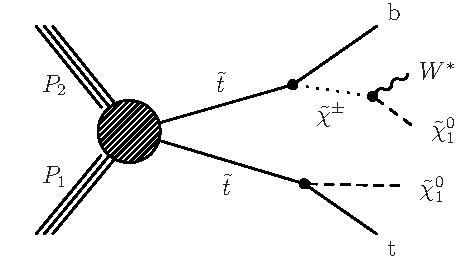
\includegraphics[height=0.15\textwidth]{figures/T2tb_feyn}
     \label{fig:T2tb_feyn}
   } ~~
   \subfigure[\texttt{T2tt}]{
     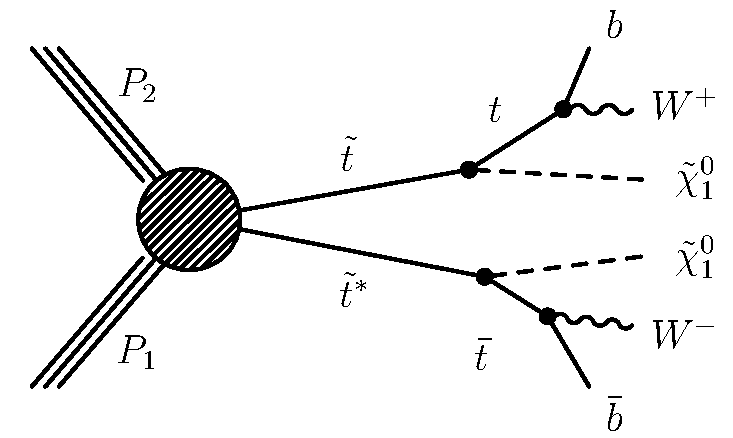
\includegraphics[height=0.15\textwidth]{figures/T2tt_feyn}
     \label{fig:T2tt_feyn}
   } \\
   \subfigure[\texttt{T2cc}]{
     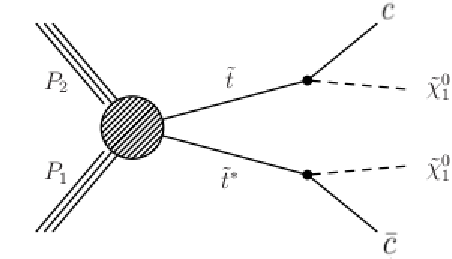
\includegraphics[height=0.15\textwidth]{figures/T2cc_feyn}
     \label{fig:T2cc_feyn}
   } ~~
   \subfigure[\texttt{T2bW\_X05}]{
     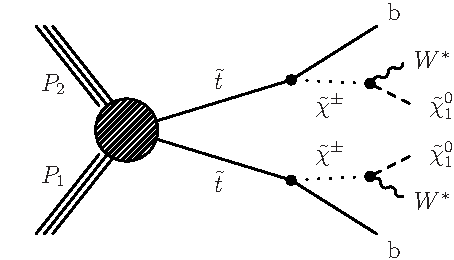
\includegraphics[height=0.15\textwidth]{figures/T2bW_X05_feyn}
     \label{fig:T2bW_X05_feyn}
   } ~~
   \caption{ Simplified model diagrams that represent unique
     production and decay modes of supersymmetric
     particles. Three-body decays of gluinos are assumed to proceed
     through off-shell squarks. The diagrams labelled
     \texttt{T1qqqq} and \texttt{T2qq} depict, respectively, the
     gluino-mediated and direct production of light-flavour
     squarks. The diagrams labelled \texttt{T1bbbb}, \texttt{T1tttt},
     and \texttt{T1ttbb} depict models involving the gluino-mediated
     production of off-shell third-generation squarks. The diagrams
     labelled \texttt{T5tttt}, \texttt{T5ttcc}, and
     \texttt{T5tttt\_degen} depict ``natural'' models comprising
     gluino-mediated production of on-shell top squarks. Finally, the
     remaining six diagrams depict the direct production of on-shell
     third-generation squarks, decaying via a range of channels.  }
   \label{fig:simplified-models}
 \end{center}
\end{figure*}


\clearpage
\begin{figure*}[t]
  \begin{center}
    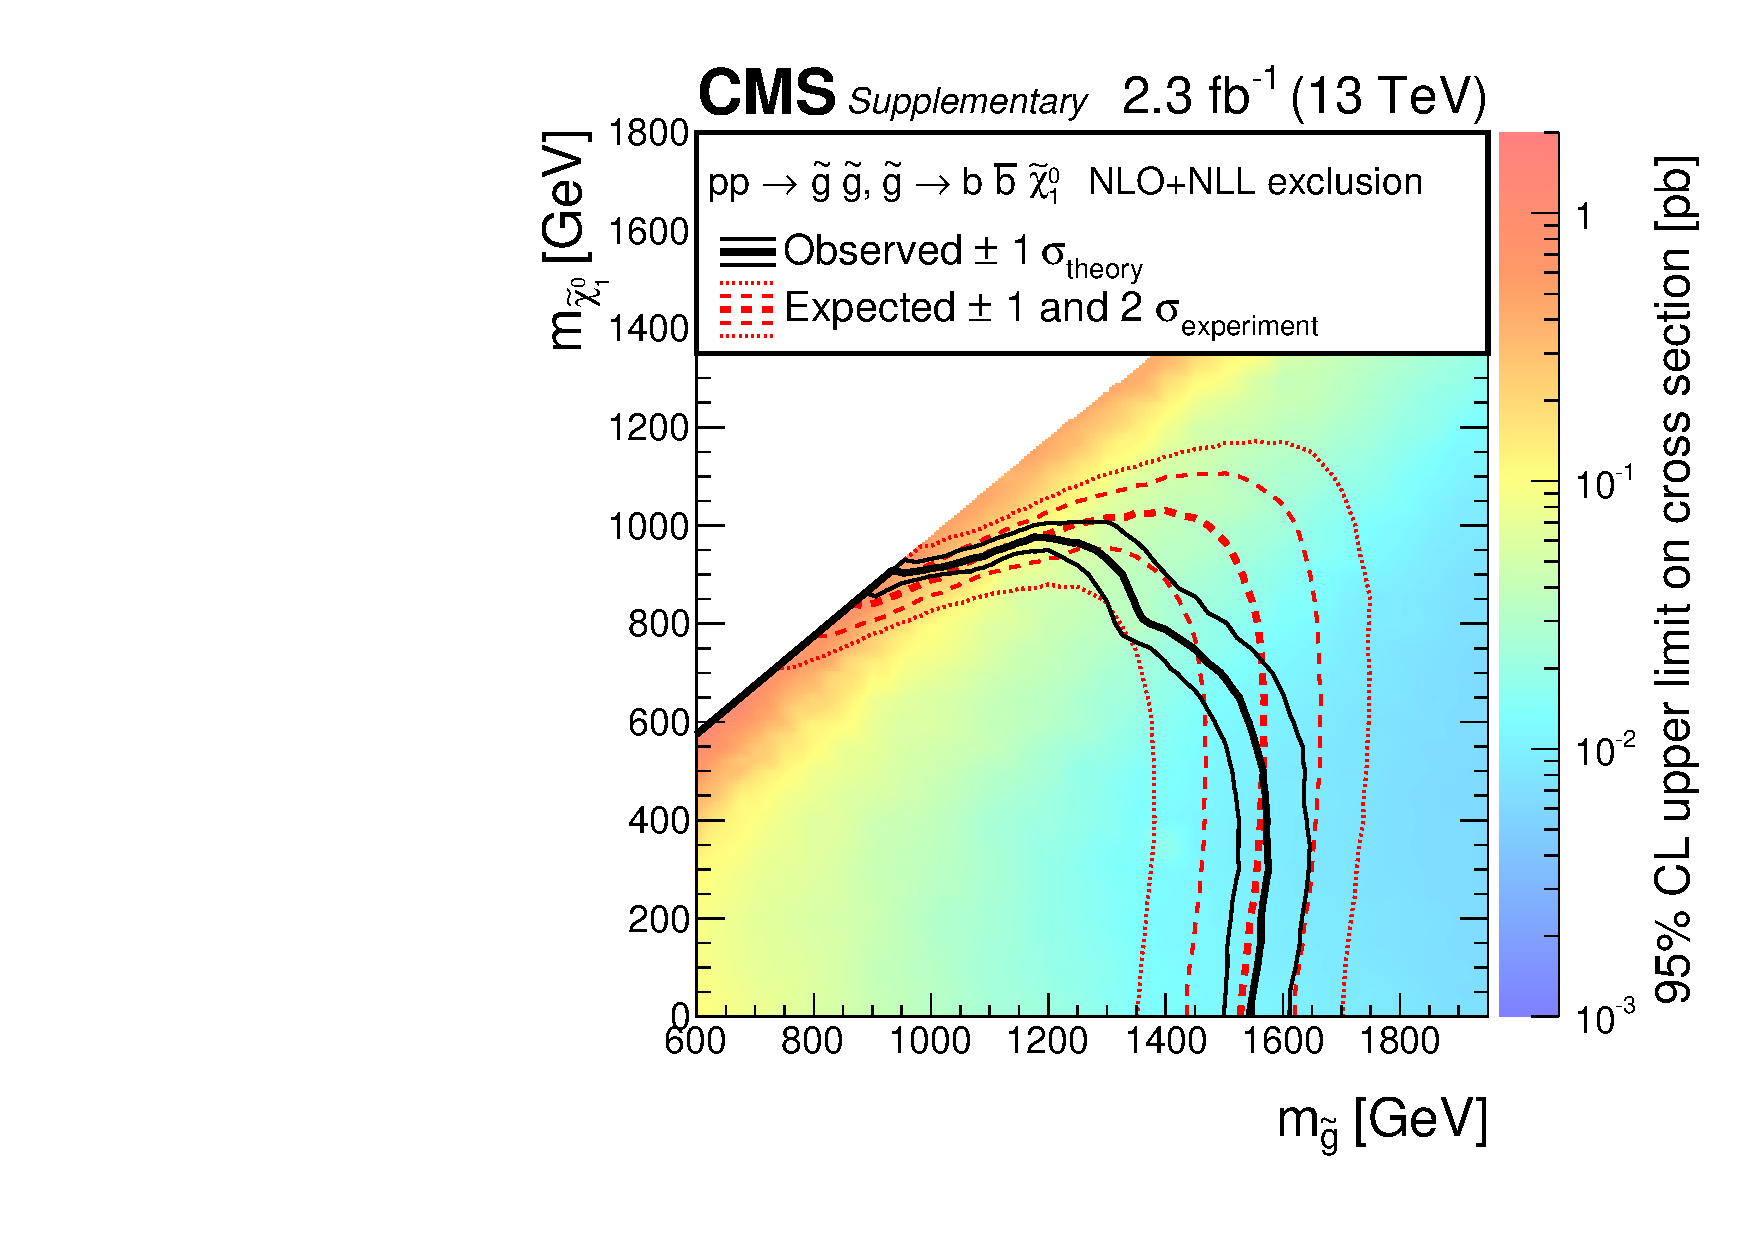
\includegraphics[width=0.49\textwidth]{supplementary/figures/RA1T1bbbbXSEC} \, 
    \includegraphics[width=0.49\textwidth]{supplementary/figures/T1bbbb_merging_4_cats} \,     
  \end{center}
  \caption{Left: (coloured histogram) upper limit on the cross section in the $(m_{\mathrm{Gluino}},m_{\mathrm{LSP}})$ plane for the T1bbbb model. 
  The black (red) solid line is the observed (expected) exclusion. The red dashed lines are the $\pm1\sigma$ expected exclusion due to experimental uncertainties. 
  The $\pm1\sigma$ observed exclusion due to theoretical uncertainties on the signal cross section are shown as thin black lines. 
  Right: signal efficiency for the search regions included in the limit calculation as a function $(m_{\mathrm{Gluino}},m_{\mathrm{LSP}})$ plane for the T1bbbb model. 
  \label{fig:T1bbbb_excl}}
\end{figure*}

\begin{figure*}[t]
  \begin{center}
    \includegraphics[width=0.49\textwidth]{supplementary/figures/RA1T1ttttXSEC} \, 
    \includegraphics[width=0.49\textwidth]{supplementary/figures/T1tttt_merging_4_cats} \,     
  \end{center}
  \caption{Left: (coloured histogram) upper limit on the cross section in the $(m_{\mathrm{Gluino}},m_{\mathrm{LSP}})$ plane for the T1tttt model. 
  The black (red) solid line is the observed (expected) exclusion. The red dashed lines are the $\pm1\sigma$ expected exclusion due to experimental uncertainties. 
  The $\pm1\sigma$ observed exclusion due to theoretical uncertainties on the signal cross section are shown as thin black lines. 
  Right: signal efficiency for the search regions included in the limit calculation as a function $(m_{\mathrm{Gluino}},m_{\mathrm{LSP}})$ plane for the T1tttt model. 
  \label{fig:T1tttt_excl}}
\end{figure*}

\clearpage
\begin{figure*}[t]
  \begin{center}
    \includegraphics[width=0.49\textwidth]{supplementary/figures/RA1T1qqqqXSEC} \, 
    \includegraphics[width=0.49\textwidth]{supplementary/figures/T1qqqq_merging_4_cats} \,     
  \end{center}
  \caption{Left: (coloured histogram) upper limit on the cross section in the $(m_{\mathrm{Gluino}},m_{\mathrm{LSP}})$ plane for the T1qqqq model. 
  The black (red) solid line is the observed (expected) exclusion. The red dashed lines are the $\pm1\sigma$ expected exclusion due to experimental uncertainties. 
  The $\pm1\sigma$ observed exclusion due to theoretical uncertainties on the signal cross section are shown as thin black lines. 
  Right: signal efficiency for the search regions included in the limit calculation as a function $(m_{\mathrm{Gluino}},m_{\mathrm{LSP}})$ plane for the T1qqqq model. 
  \label{fig:T1qqqq_excl}}
\end{figure*}

\begin{figure*}[t]
  \begin{center}
    \includegraphics[width=0.49\textwidth]{supplementary/figures/RA1T1ttbbXSEC} \, 
    \includegraphics[width=0.49\textwidth]{supplementary/figures/T1ttbb_merging_4_cats} \,     
  \end{center}
  \caption{Left: (coloured histogram) upper limit on the cross section in the $(m_{\mathrm{Gluino}},m_{\mathrm{LSP}})$ plane for the T1ttbb model. 
  The black (red) solid line is the observed (expected) exclusion. The red dashed lines are the $\pm1\sigma$ expected exclusion due to experimental uncertainties. 
  The $\pm1\sigma$ observed exclusion due to theoretical uncertainties on the signal cross section are shown as thin black lines. 
  Right: signal efficiency for the search regions included in the limit calculation as a function $(m_{\mathrm{Gluino}},m_{\mathrm{LSP}})$ plane for the T1ttbb model. 
  \label{fig:T1ttbb_excl}}
\end{figure*}


\clearpage
\begin{figure*}[t]
  \begin{center}
    \includegraphics[width=0.49\textwidth]{supplementary/figures/RA1T5ttccXSEC} \, 
    \includegraphics[width=0.49\textwidth]{supplementary/figures/T5ttcc_merging_4_cats} \,     
  \end{center}
  \caption{Left: (coloured histogram) upper limit on the cross section in the $(m_{\mathrm{Gluino}},m_{\mathrm{LSP}})$ plane for the T5ttcc model. 
  The black (red) solid line is the observed (expected) exclusion. The red dashed lines are the $\pm1\sigma$ expected exclusion due to experimental uncertainties. 
  The $\pm1\sigma$ observed exclusion due to theoretical uncertainties on the signal cross section are shown as thin black lines. 
  Right: signal efficiency for the search regions included in the limit calculation as a function $(m_{\mathrm{Gluino}},m_{\mathrm{LSP}})$ plane for the T5ttcc model. 
  \label{fig:T5ttcc_excl}}
\end{figure*}

\begin{figure*}[t]
  \begin{center}
    \includegraphics[width=0.49\textwidth]{supplementary/figures/RA1T5ttttDM175XSEC} \, 
    \includegraphics[width=0.49\textwidth]{supplementary/figures/T5ttttDM175_merging_4_cats} \,     
  \end{center}
  \caption{Left: (coloured histogram) upper limit on the cross section in the $(m_{\mathrm{Gluino}},m_{\mathrm{LSP}})$ plane for the T5ttttDM175 model. 
  The black (red) solid line is the observed (expected) exclusion. The red dashed lines are the $\pm1\sigma$ expected exclusion due to experimental uncertainties. 
  The $\pm1\sigma$ observed exclusion due to theoretical uncertainties on the signal cross section are shown as thin black lines. 
  Right: signal efficiency for the search regions included in the limit calculation as a function $(m_{\mathrm{Gluino}},m_{\mathrm{LSP}})$ plane for the T5ttttDM175 model. 
  \label{fig:T5ttttDM175_excl}}
\end{figure*}


\clearpage
\begin{figure*}[t]
  \begin{center}
    \includegraphics[width=0.49\textwidth]{supplementary/figures/RA1T5tttt-degenXSEC} \, 
    \includegraphics[width=0.49\textwidth]{supplementary/figures/T5tttt_degen_merging_4_cats} \,     
  \end{center}
  \caption{Left: (coloured histogram) upper limit on the cross section in the $(m_{\mathrm{Gluino}},m_{\mathrm{LSP}})$ plane for the T5tttt\_degen model. 
  The black (red) solid line is the observed (expected) exclusion. The red dashed lines are the $\pm1\sigma$ expected exclusion due to experimental uncertainties. 
  The $\pm1\sigma$ observed exclusion due to theoretical uncertainties on the signal cross section are shown as thin black lines. 
  Right: signal efficiency for the search regions included in the limit calculation as a function $(m_{\mathrm{Gluino}},m_{\mathrm{LSP}})$ plane for the T5tttt\_degen model. 
  \label{fig:T5tttt_degen_excl}}
\end{figure*}

\begin{figure*}[t]
  \begin{center}
    \includegraphics[width=0.49\textwidth]{supplementary/figures/RA1T2ttXSEC} \, 
    \includegraphics[width=0.49\textwidth]{supplementary/figures/T2tt_merging_4_cats} \,     
  \end{center}
  \caption{Left: (coloured histogram) upper limit on the cross section in the $(m_{\mathrm{Gluino}},m_{\mathrm{LSP}})$ plane for the T2tt model. 
  The black (red) solid line is the observed (expected) exclusion. The red dashed lines are the $\pm1\sigma$ expected exclusion due to experimental uncertainties. 
  The $\pm1\sigma$ observed exclusion due to theoretical uncertainties on the signal cross section are shown as thin black lines. 
  Right: signal efficiency for the search regions included in the limit calculation as a function $(m_{\mathrm{Gluino}},m_{\mathrm{LSP}})$ plane for the T2tt model. 
  \label{fig:T2tt_excl}}
\end{figure*}


\clearpage
\begin{figure*}[t]
  \begin{center}
    \includegraphics[width=0.49\textwidth]{supplementary/figures/RA1T2ccXSEC} \, 
    \includegraphics[width=0.49\textwidth]{supplementary/figures/T2cc_merging_4_cats} \,     
  \end{center}
  \caption{Left: (coloured histogram) upper limit on the cross section in the $(m_{\mathrm{Gluino}},m_{\mathrm{LSP}})$ plane for the T2cc model. 
  The black (red) solid line is the observed (expected) exclusion. The red dashed lines are the $\pm1\sigma$ expected exclusion due to experimental uncertainties. 
  The $\pm1\sigma$ observed exclusion due to theoretical uncertainties on the signal cross section are shown as thin black lines. 
  Right: signal efficiency for the search regions included in the limit calculation as a function $(m_{\mathrm{Gluino}},m_{\mathrm{LSP}})$ plane for the T2cc model. 
  \label{fig:T2cc_excl}}
\end{figure*}

\begin{figure*}[t]
  \begin{center}
    \includegraphics[width=0.49\textwidth]{supplementary/figures/RA1T2-4bdXSEC} \, 
    \includegraphics[width=0.49\textwidth]{supplementary/figures/T2-4bd_merging_4_cats} \,     
  \end{center}
  \caption{Left: (coloured histogram) upper limit on the cross section in the $(m_{\mathrm{Gluino}},m_{\mathrm{LSP}})$ plane for the T2-4bd model. 
  The black (red) solid line is the observed (expected) exclusion. The red dashed lines are the $\pm1\sigma$ expected exclusion due to experimental uncertainties. 
  The $\pm1\sigma$ observed exclusion due to theoretical uncertainties on the signal cross section are shown as thin black lines. 
  Right: signal efficiency for the search regions included in the limit calculation as a function $(m_{\mathrm{Gluino}},m_{\mathrm{LSP}})$ plane for the T2-4bd model. 
  \label{fig:T2-4bd_excl}}
\end{figure*}


\clearpage
\begin{figure*}[t]
  \begin{center}
    \includegraphics[width=0.49\textwidth]{supplementary/figures/RA1T2mixedXSEC} \, 
    \includegraphics[width=0.49\textwidth]{supplementary/figures/T2mixed_merging_4_cats} \,     
  \end{center}
  \caption{Left: (coloured histogram) upper limit on the cross section in the $(m_{\mathrm{Gluino}},m_{\mathrm{LSP}})$ plane for the T2mixed model. 
  The black (red) solid line is the observed (expected) exclusion. The red dashed lines are the $\pm1\sigma$ expected exclusion due to experimental uncertainties. 
  The $\pm1\sigma$ observed exclusion due to theoretical uncertainties on the signal cross section are shown as thin black lines. 
  Right: signal efficiency for the search regions included in the limit calculation as a function $(m_{\mathrm{Gluino}},m_{\mathrm{LSP}})$ plane for the T2mixed model. 
  \label{fig:T2mixed_excl}}
\end{figure*}

\begin{figure*}[t]
  \begin{center}
    \includegraphics[width=0.49\textwidth]{supplementary/figures/RA1T2tbXSEC} \, 
    \includegraphics[width=0.49\textwidth]{supplementary/figures/T2tb_merging_4_cats} \,     
  \end{center}
  \caption{Left: (coloured histogram) upper limit on the cross section in the $(m_{\mathrm{Gluino}},m_{\mathrm{LSP}})$ plane for the T2tb model. 
  The black (red) solid line is the observed (expected) exclusion. The red dashed lines are the $\pm1\sigma$ expected exclusion due to experimental uncertainties. 
  The $\pm1\sigma$ observed exclusion due to theoretical uncertainties on the signal cross section are shown as thin black lines. 
  Right: signal efficiency for the search regions included in the limit calculation as a function $(m_{\mathrm{Gluino}},m_{\mathrm{LSP}})$ plane for the T2tb model. 
  \label{fig:T2tb_excl}}
\end{figure*}


\clearpage
\begin{figure*}[t]
  \begin{center}
    \includegraphics[width=0.49\textwidth]{supplementary/figures/RA1T2bW-X05XSEC} \, 
    \includegraphics[width=0.49\textwidth]{supplementary/figures/T2bW_X05_merging_4_cats} \,     
  \end{center}
  \caption{Left: (coloured histogram) upper limit on the cross section in the $(m_{\mathrm{Gluino}},m_{\mathrm{LSP}})$ plane for the T2bW\_X05 model. 
  The black (red) solid line is the observed (expected) exclusion. The red dashed lines are the $\pm1\sigma$ expected exclusion due to experimental uncertainties. 
  The $\pm1\sigma$ observed exclusion due to theoretical uncertainties on the signal cross section are shown as thin black lines. 
  Right: signal efficiency for the search regions included in the limit calculation as a function $(m_{\mathrm{Gluino}},m_{\mathrm{LSP}})$ plane for the T2bW\_X05 model. 
  \label{fig:T2bW_X05_excl}}
\end{figure*}

\begin{figure*}[t]
  \begin{center}
    \includegraphics[width=0.49\textwidth]{supplementary/figures/RA1T2bbXSEC} \, 
    \includegraphics[width=0.49\textwidth]{supplementary/figures/T2bb_merging_4_cats} \,     
  \end{center}
  \caption{Left: (coloured histogram) upper limit on the cross section in the $(m_{\mathrm{Gluino}},m_{\mathrm{LSP}})$ plane for the T2bb model. 
  The black (red) solid line is the observed (expected) exclusion. The red dashed lines are the $\pm1\sigma$ expected exclusion due to experimental uncertainties. 
  The $\pm1\sigma$ observed exclusion due to theoretical uncertainties on the signal cross section are shown as thin black lines. 
  Right: signal efficiency for the search regions included in the limit calculation as a function $(m_{\mathrm{Gluino}},m_{\mathrm{LSP}})$ plane for the T2bb model. 
  \label{fig:T2bb_excl}}
\end{figure*}


\clearpage
\begin{figure*}[t]
  \begin{center}
    \includegraphics[width=0.49\textwidth]{supplementary/figures/RA1T2qqXSEC} \, 
    \includegraphics[width=0.49\textwidth]{supplementary/figures/T2qq_merging_4_cats} \,     
  \end{center}
  \caption{Left: (coloured histogram) upper limit on the cross section in the $(m_{\mathrm{Gluino}},m_{\mathrm{LSP}})$ plane for the T2qq model. 
  The black (red) solid line is the observed (expected) exclusion. The red dashed lines are the $\pm1\sigma$ expected exclusion due to experimental uncertainties. 
  The $\pm1\sigma$ observed exclusion due to theoretical uncertainties on the signal cross section are shown as thin black lines. 
  Right: signal efficiency for the search regions included in the limit calculation as a function $(m_{\mathrm{Gluino}},m_{\mathrm{LSP}})$ plane for the T2qq model. 
  \label{fig:T2qq_excl}}
\end{figure*}




\clearpage
\begin{figure*}[thp!]
  \begin{center}
    \includegraphics[width=0.49\textwidth]{figures/mixSUMMARY_transposed.pdf}
    \includegraphics[width=0.49\textwidth]{figures/gluinoSUMMARY_transposed.pdf} \\
    \includegraphics[width=0.49\textwidth]{figures/naturalSUMMARY_transposed.pdf}
    \includegraphics[width=0.49\textwidth]{figures/allThirdGenSUMMARY_transposed.pdf} \\
    \caption{Summary for the observed (solid lines) and expected (dashed lines) exclusions in the $m_{\mathrm{Susy}},m_{\mathrm{Susy}}-m_{\mathrm{LSP}}$ plane for the models considered in the analysis. 
       Exclusion contours are grouped into 4 summary plots: 
       ``Direct and gluino-mediated production of off-shell (decoupled) light-flavour squarks'' (top left), ``Gluino-mediated production of off-shell (decoupled) 3rd generation squarks'' (top right), ``Gluino-mediated production of on-shell stops and charginos (natural models)'' (bottom left), ``Direct production of 3rd generation squarks'' (bottom right). 
      \label{fig:summary-excl-plots} }
  \end{center}
\end{figure*}



\clearpage
% \nocite{*}
\bibliography{auto_generated}
